\documentclass{article}
\usepackage[utf8]{inputenc}
\usepackage{geometry}
 \geometry{
 a4paper,
 total={170mm,257mm},
 left=20mm,
 top=20mm,
 }
\usepackage{graphicx}
\usepackage{amsmath}
\usepackage{amsfonts}
\usepackage{amssymb}
\usepackage{caption}
\usepackage{subcaption}
\usepackage{listings}
\usepackage{xcolor}

 \title{Computer Vision Assignment 4
}
\author{Madhia Shabih}
\date{September 2024}
  
\makeatletter
\def\@maketitle{%
  \newpage
  \null
  \vskip 1em%
  \begin{center}%
  \let \footnote \thanks
    {\LARGE \@title \par}%
    \vskip 1em%
    %{\large \@date}%
  \end{center}%
  \par
  \vskip 1em}
\makeatother

\usepackage{lipsum}  
\usepackage{cmbright}

\begin{document}

\maketitle

\noindent\begin{tabular}{@{}ll}
    Student & \author\\
     
\end{tabular}

\section{Estimating a Camera Matrix Pair and Reconstructing 3D Features}

\subsection{Problem Description}
%Describe the task of estimating camera matrices from the image pair, including the use of SIFT feature matches and the provided calibration matrix. 
Estimating camera matrices from an image pair involves determining the relative positions and orientations of the cameras that captured the images. 
This is done using corresponding feature points between the two images, detected through SIFT (Scale-Invariant Feature Transform) feature matching. 
The provided 3x3 calibration matrix, which describes the intrinsic parameters of the cameras (such as focal length and optical center), is used to refine the estimation process.
By accurately estimating these camera matrices, the 3D structure of the scene can be inferred from the 2D image pair.
\textbf{Aim}: Estimate the spatial relationship between cameras and reconstruct the 3D coordinates of features.

\subsection{Part (a): Feature Matches}
\textbf{Description}: %Explain how feature matches were displayed and how obvious errors were removed.
In the file \texttt{q1.py}, in the function \texttt{plot\_matches}, I visualize feature matches between two images. 
I first convert the input image to grayscale using OpenCV. Then I filter the matches based on a maximum allowed distance between matched points using a helper function called \texttt{filter\_matches}. 
I use a distance of 50. A matplotlib figure is created to display the grayscale image, and for each pair of matched coordinates (x1, y1) and (x2, y2), 
a red line is drawn between the points, while a blue circle is placed at the first point (x1, y1) for clarity.

\textbf{Discussion}: %Justify why a lenient threshold was used to retain incorrect matches. Discuss implications for further steps.
Since further refinement techniques, such as the RANSAC algorithm, will filter out incorrect matches, its more effective to start with a larger set of matches.
This could reduce the accuracy of the final camera matrix estimation and 3D reconstruction. Hence, is more critical to preserve as many potentially correct matches than 
prematurely discarding data. 

\begin{figure}[h!]
    \centering
    % First subfigure
    \begin{subfigure}[b]{0.45\textwidth}
        \centering
        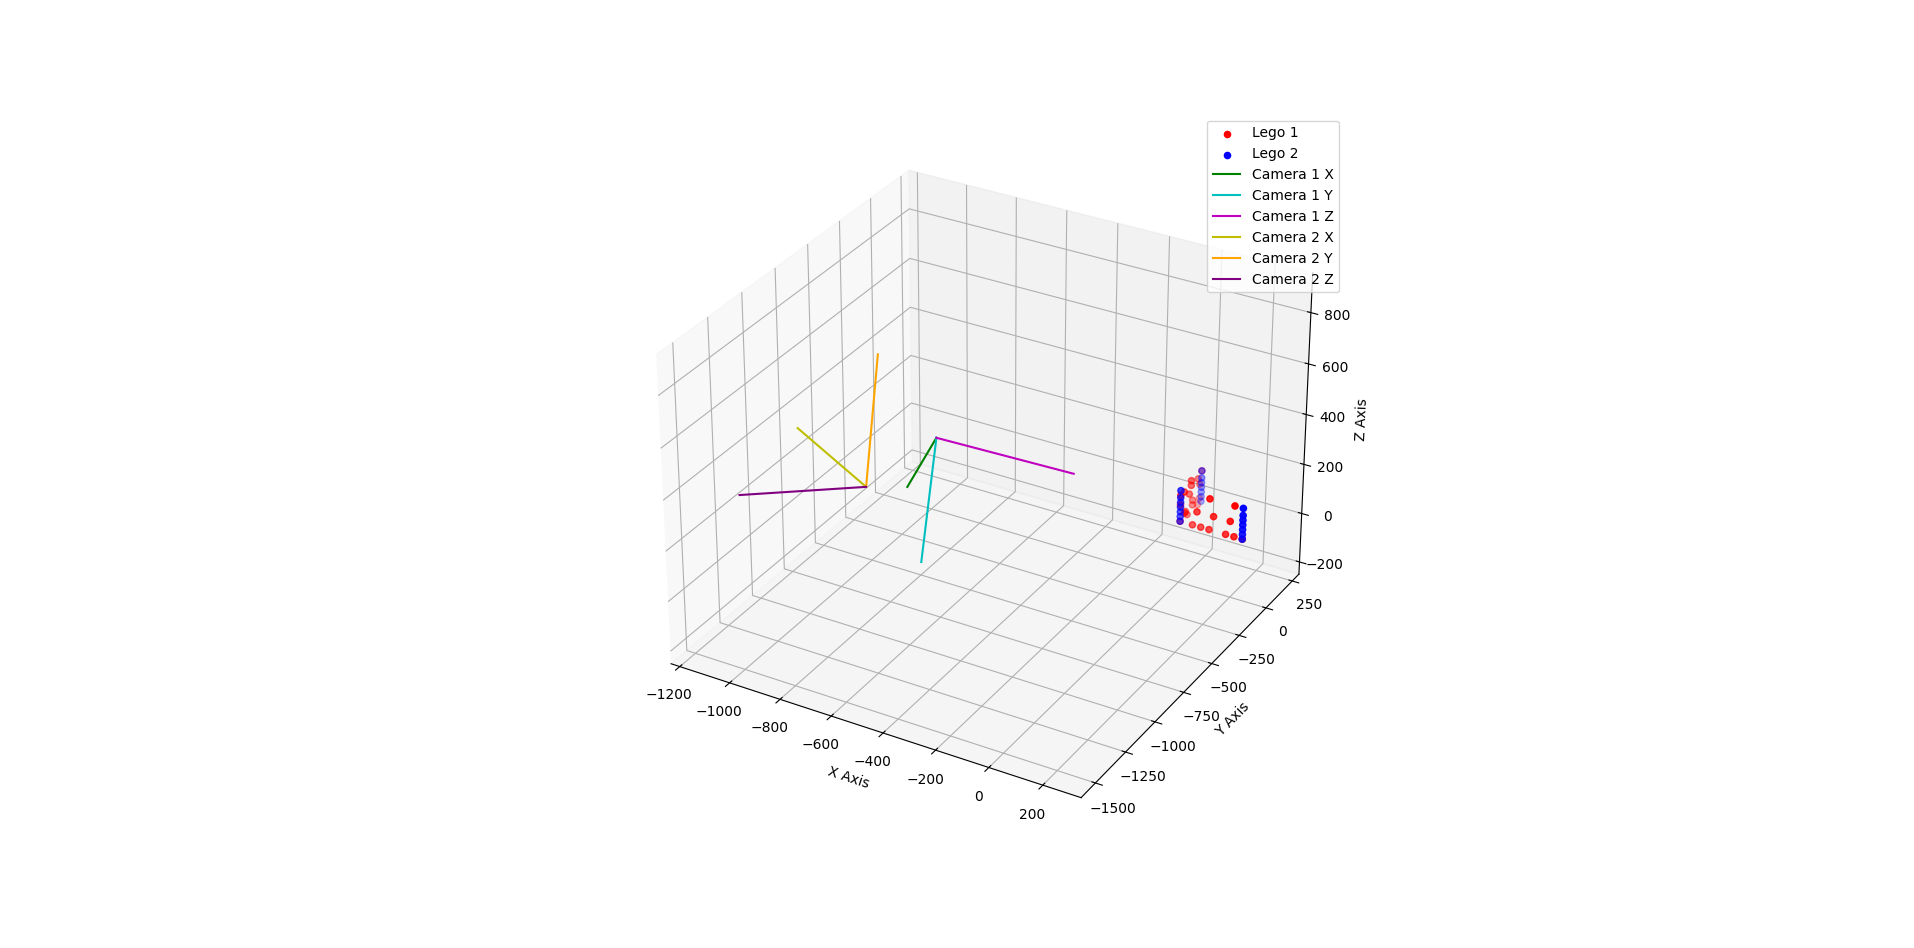
\includegraphics[trim={15cm 0 15cm 0}, clip, width=\textwidth]{/home/madhia/computer_vision/assignment4/implementation/q1-2/output/Figure_1.png}
        \caption{All feature matches.}
        \label{fig:first}
    \end{subfigure}
    \hfill
    % Second subfigure
    \begin{subfigure}[b]{0.45\textwidth}
        \centering
        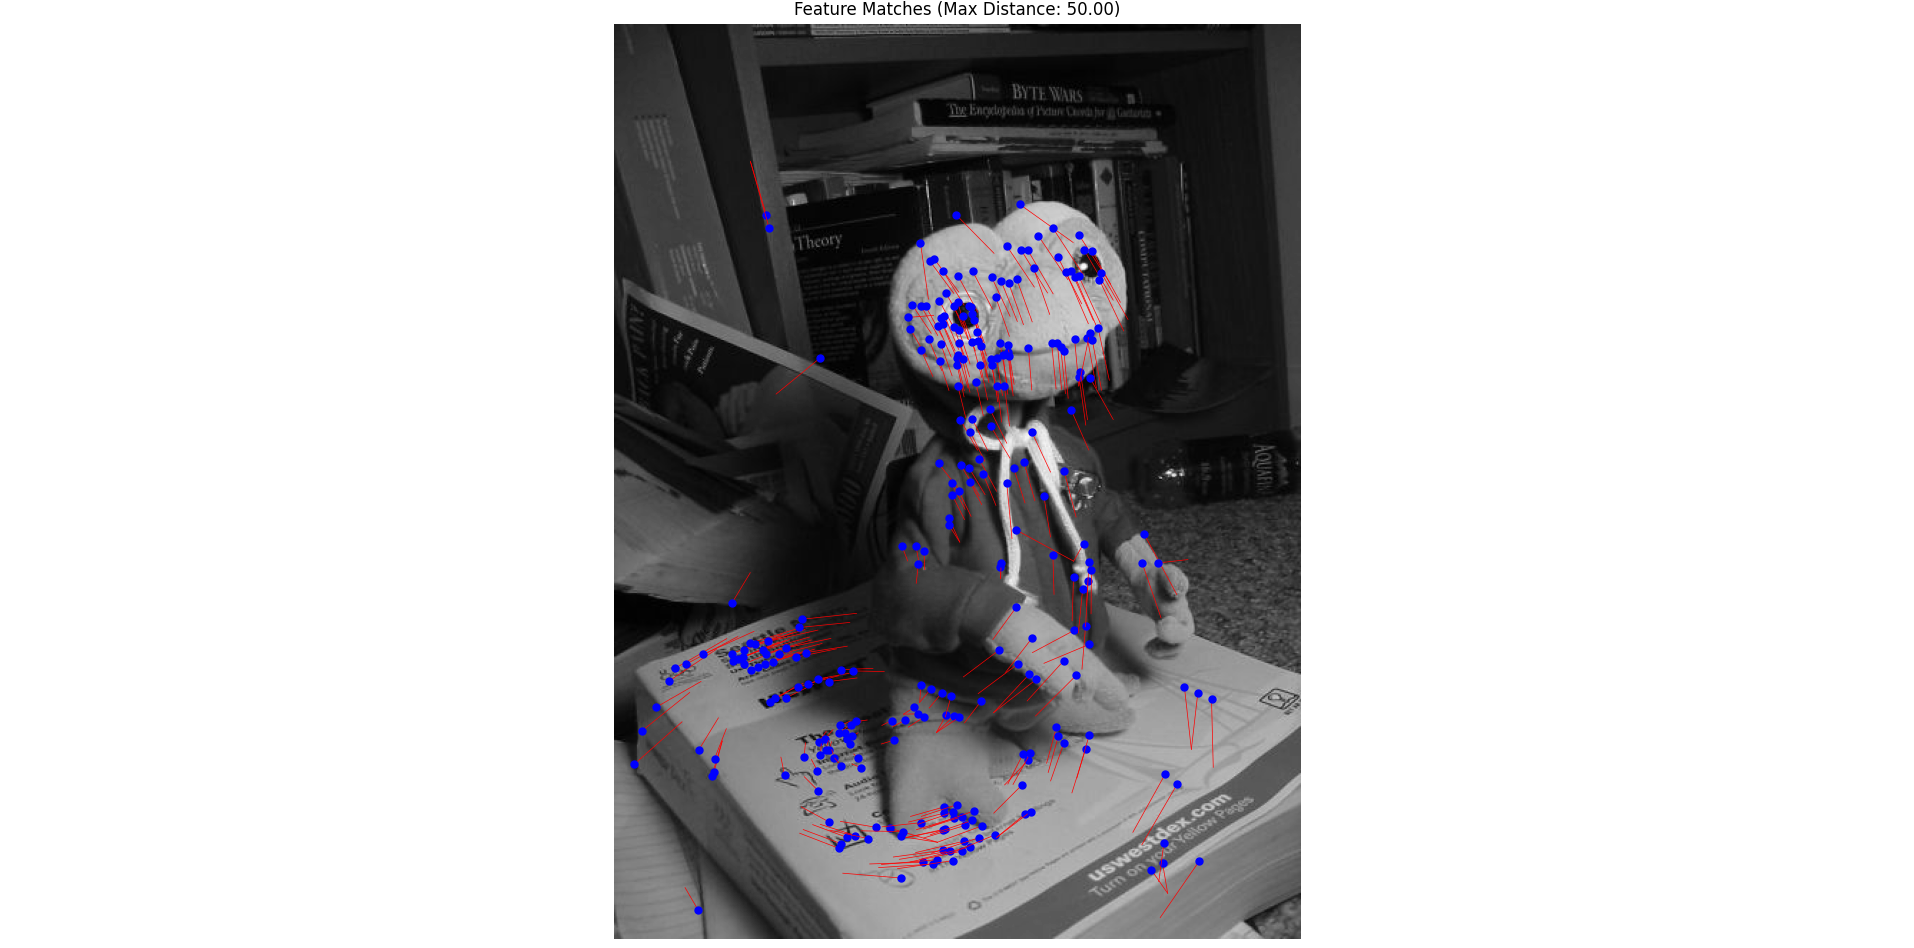
\includegraphics[   trim={15cm 0 15cm 0}, clip, width=\textwidth]{/home/madhia/computer_vision/assignment4/implementation/q1-2/output/Figure_2.png}
        \caption{Feature matches within a maximum distance of 50.}
        \label{fig:second}
    \end{subfigure}
    
    \caption{Feature matches displayed on greyscale image.}
    \label{fig:overall}
\end{figure}

\subsection{Part (b): Estimating the Fundamental Matrix using RANSAC}
\textbf{Description}: %Explain the RANSAC procedure to estimate the fundamental matrix.
RANSAC is used to enhance the accuracy by estimating the best fundamental matrix from the noisy data which means defining the inliers. 
The \texttt{ransac} function is an implementation of the RANSAC (Random Sample Consensus) algorithm used to estimate the best-fit fundamental matrix from a set of point correspondences between two images.
Given a set of matches, a distance threshold, and a specified number of iterations, it iteratively selects random subsets of points to compute candidate fundamental matrices. 
The algorithm then calculates the Sampson distance to determine inliers, which are points fitting the model well within the given threshold. 
If the number of inliers exceeds the maximum found so far, the current matrix is saved as the best model. 
Finally, the function outputs the inliers from both sets of points along with the corresponding fundamental matrix.
\textbf{Results}: %Present the final inlier matches after RANSAC, and explain why the fundamental matrix is re-estimated with all inliers.

\begin{figure}[h!]
    \centering
    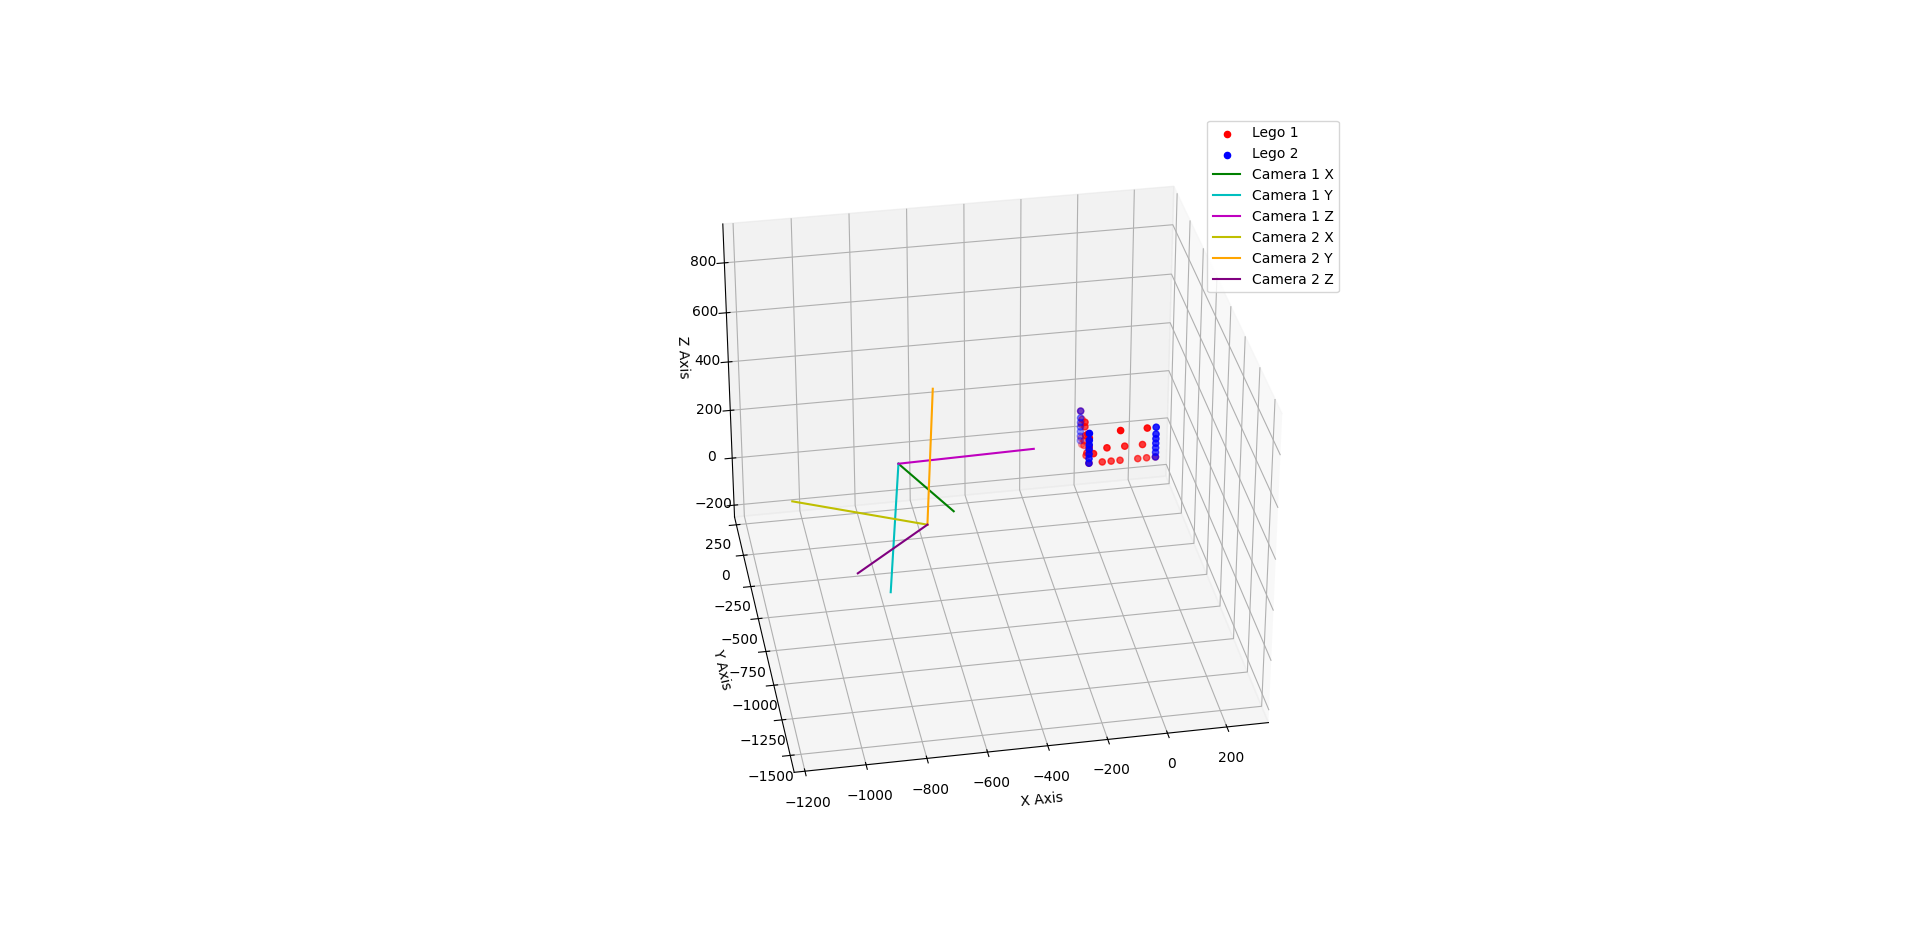
\includegraphics[trim={15cm 0 15cm 0}, clip, width=0.8\textwidth]{/home/madhia/computer_vision/assignment4/implementation/q1-2/output/Figure_3.png}
    \caption{Inlier matches after RANSAC.}
\end{figure}

\textit{Fundamental Matrix $\mathbf{F}$}
\[
\mathbf{F} = \begin{bmatrix} 
3.01507500 \times 10^{-6} & 1.41342356 \times 10^{-5} & -6.15058393 \times 10^{-3} \\ 
-5.21158678 \times 10^{-6} & 2.16619468 \times 10^{-6} & -3.34960812 \times 10^{-2} \\ 
7.01890584 \times 10^{-3} & 2.82974891 \times 10^{-2} & 1 
\end{bmatrix}
\]

\textbf{Discussion}: %Discuss the rationale behind re-estimating the fundamental matrix using all inliers.
The inlier matches are those that define the relationship defined by the fundamental matrix with minimal error. The fundamental matrix is re-estimated using all the inliers
because the initial estimation using RANSAC is based on a subset of points. 
Re-estimating the fundamental matrix using all inliers ensures that it is refined using the full set of reliable correspondences.

\subsection{Part (c): Essential Matrix and SVD Decomposition}
\textbf{Description}: %Explain how the essential matrix is computed from the fundamental matrix and calibration matrix.
The essential matrix is computed as follows:
\[
E = K'^{T} F K
\]
where $K$ is the calibration matrix and $F$ is the fundamental matrix.

The \texttt{compute\_essential\_matrix} function calculates the essential matrix $E$ using the fundamental matrix $F$ and the camera intrinsic matrices $K$ and $K2$. 
It first computes $E$ as $E = K2^{T} \cdot F \cdot K$. Then, it performs Singular Value Decomposition (SVD) on $E$ to obtain matrices $U$, $S$, and $V^{T}$. 
If the determinants of $U$ and $V^{T}$ suggest an improper rotation, the function corrects the sign of $E$, $U$, or $V^{T}$ as needed. 
The function returns the essential matrix along with its SVD components.

\textbf{Results}: %Show the singular values of the essential matrix and discuss any discrepancies from the theoretical expectation.

\textit{Essential Matrix $\mathbf{E}$}
\[
\mathbf{E} = \begin{bmatrix}
1.40498738 & 6.58637766 & -0.61125391 \\ 
-2.4285345 & 1.00941973 & -23.24719819 \\ 
4.146119 & 22.11118505 & 0.62734739 
\end{bmatrix}
\]

\textit{Matrix $\mathbf{U}$}
\[
\mathbf{U} = \begin{bmatrix}
0.26672047 & -0.10761536 & -0.9577469 \\ 
0.46992722 & 0.88213399 & 0.03174956 \\ 
0.84144435 & -0.45853959 & 0.28585458 
\end{bmatrix}
\]

\textit{Singular Values (S)}
\[
\mathbf{S} = \begin{bmatrix}
23.51749503 & 0 & 0 \\ 
0 & 23.37591927 & 0 \\ 
0 & 0 & 0.24314841 
\end{bmatrix}
\]

\textit{Matrix $\mathbf{V}^T$}
\[
\mathbf{V}^T = \begin{bmatrix}
0.11575352 & 0.88599604 & -0.44901241 \\ 
-0.17944324 & -0.42595996 & -0.88676842 \\ 
-0.97693462 & 0.18321881 & 0.10967964 
\end{bmatrix}
\]

%\textbf{Discussion}: Discuss how the SVD algorithm may return orthogonal matrices with undesirable reflections and how the correction was applied.

\subsection{Part (d): Determining Camera Matrices}
\textbf{Description}: Explain how two camera matrices are determined from the essential matrix.

\textbf{Results}: 

\textit{Projection Matrix $\mathbf{P}$}
\[
\mathbf{P} = \begin{bmatrix}
682.6328 & 0 & 240.5 & 0 \\ 
0 & 682.6328 & 320.5 & 0 \\ 
0 & 0 & 1 & 0 
\end{bmatrix}
\]

\textit{Projection Matrix $\mathbf{P}'$}
\[
\mathbf{P}' = \begin{bmatrix}
6.19263674 \times 10^{2} & -1.06228151 \times 10^{2} & 3.59243472 \times 10^{2} & -5.85041422 \times 10^{2} \\ 
4.79717086 \times 10^{1} & 6.75589380 \times 10^{2} & 3.31640611 \times 10^{2} & 1.13289682 \times 10^{2} \\ 
-1.81347303 \times 10^{-1} & 4.53128221 \times 10^{-3} & 9.83408676 \times 10^{-1} & 2.85854580 \times 10^{-1} 
\end{bmatrix}
\]

\textbf{Discussion}: Briefly discuss how these matrices relate to the camera positions and orientations.

\subsection{Part (e): Triangulation and 3D Reconstruction}
\textbf{Description}: Describe the triangulation process to determine 3D coordinates of inlier matches.

\textbf{Results}: Showcase your 3D reconstruction, including the positions of the cameras and the 3D points.

\begin{figure}[h!]
    \centering
    \begin{minipage}{0.4\textwidth}
        \centering
        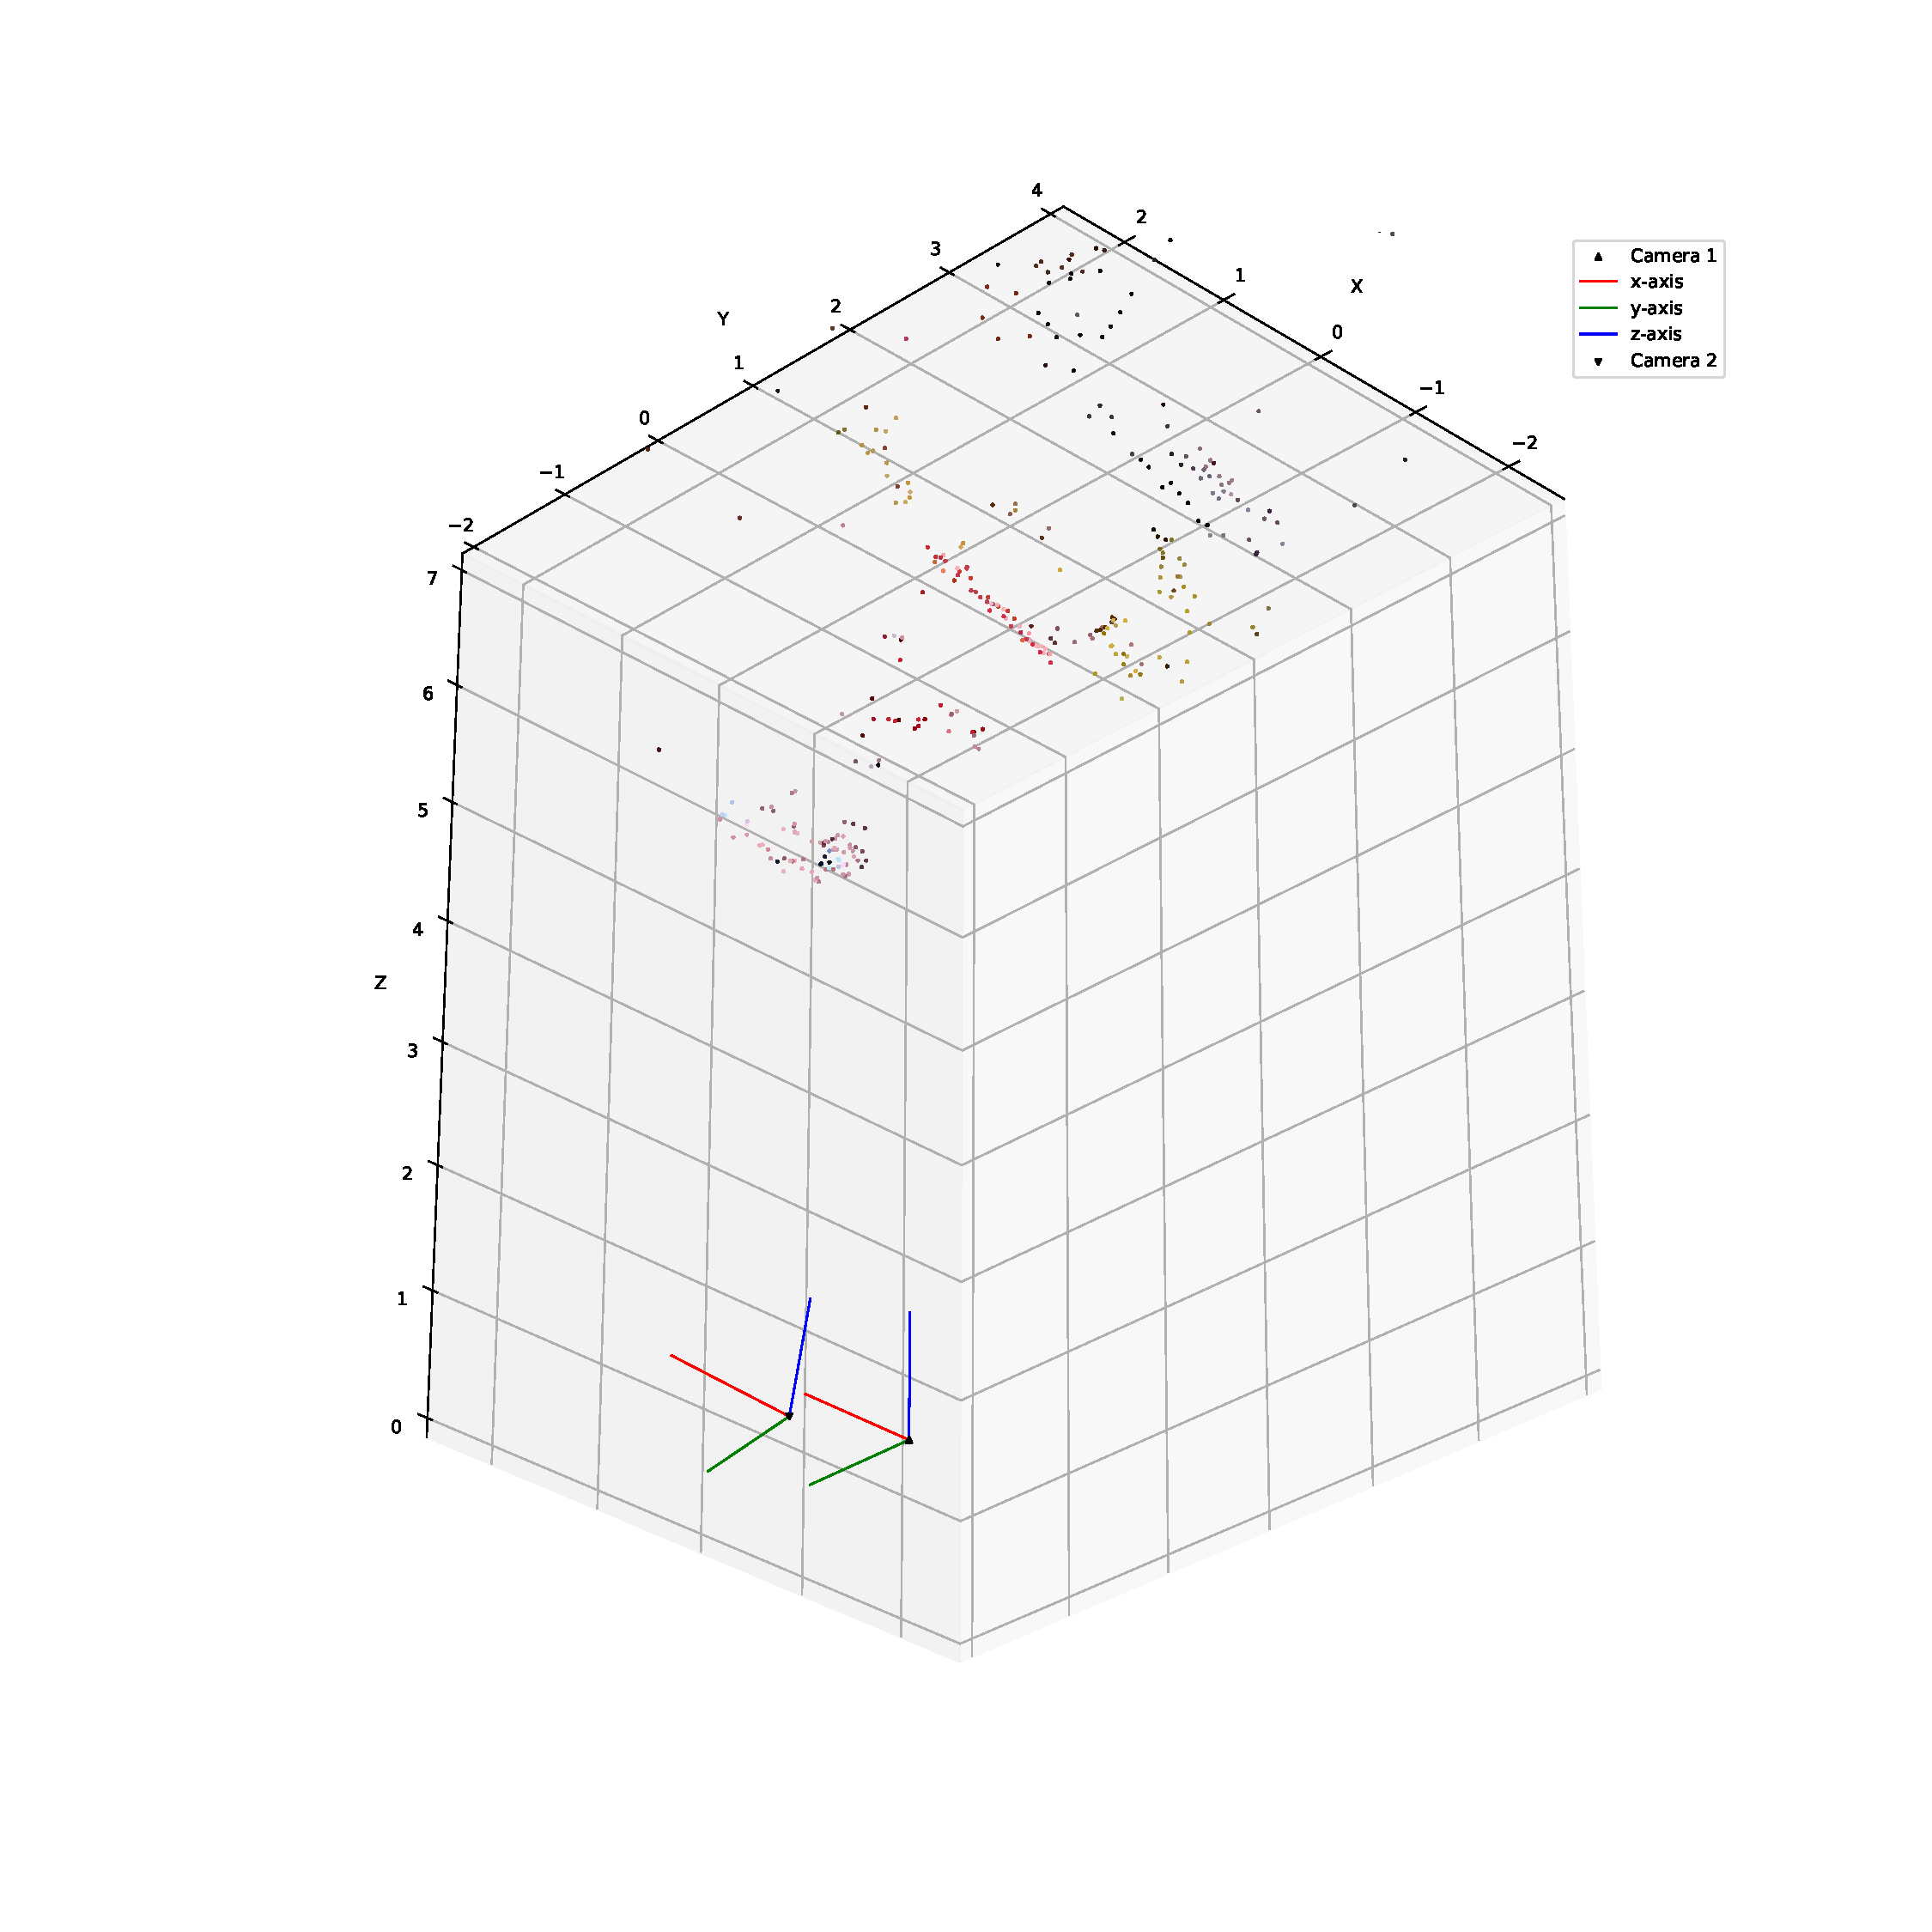
\includegraphics[width=\linewidth]{/home/madhia/computer_vision/assignment4/implementation/q1-2/output/et_3d_-30-45.pdf}
        \caption{Figure 1}
    \end{minipage}%
    \begin{minipage}{0.4\textwidth}
        \centering
        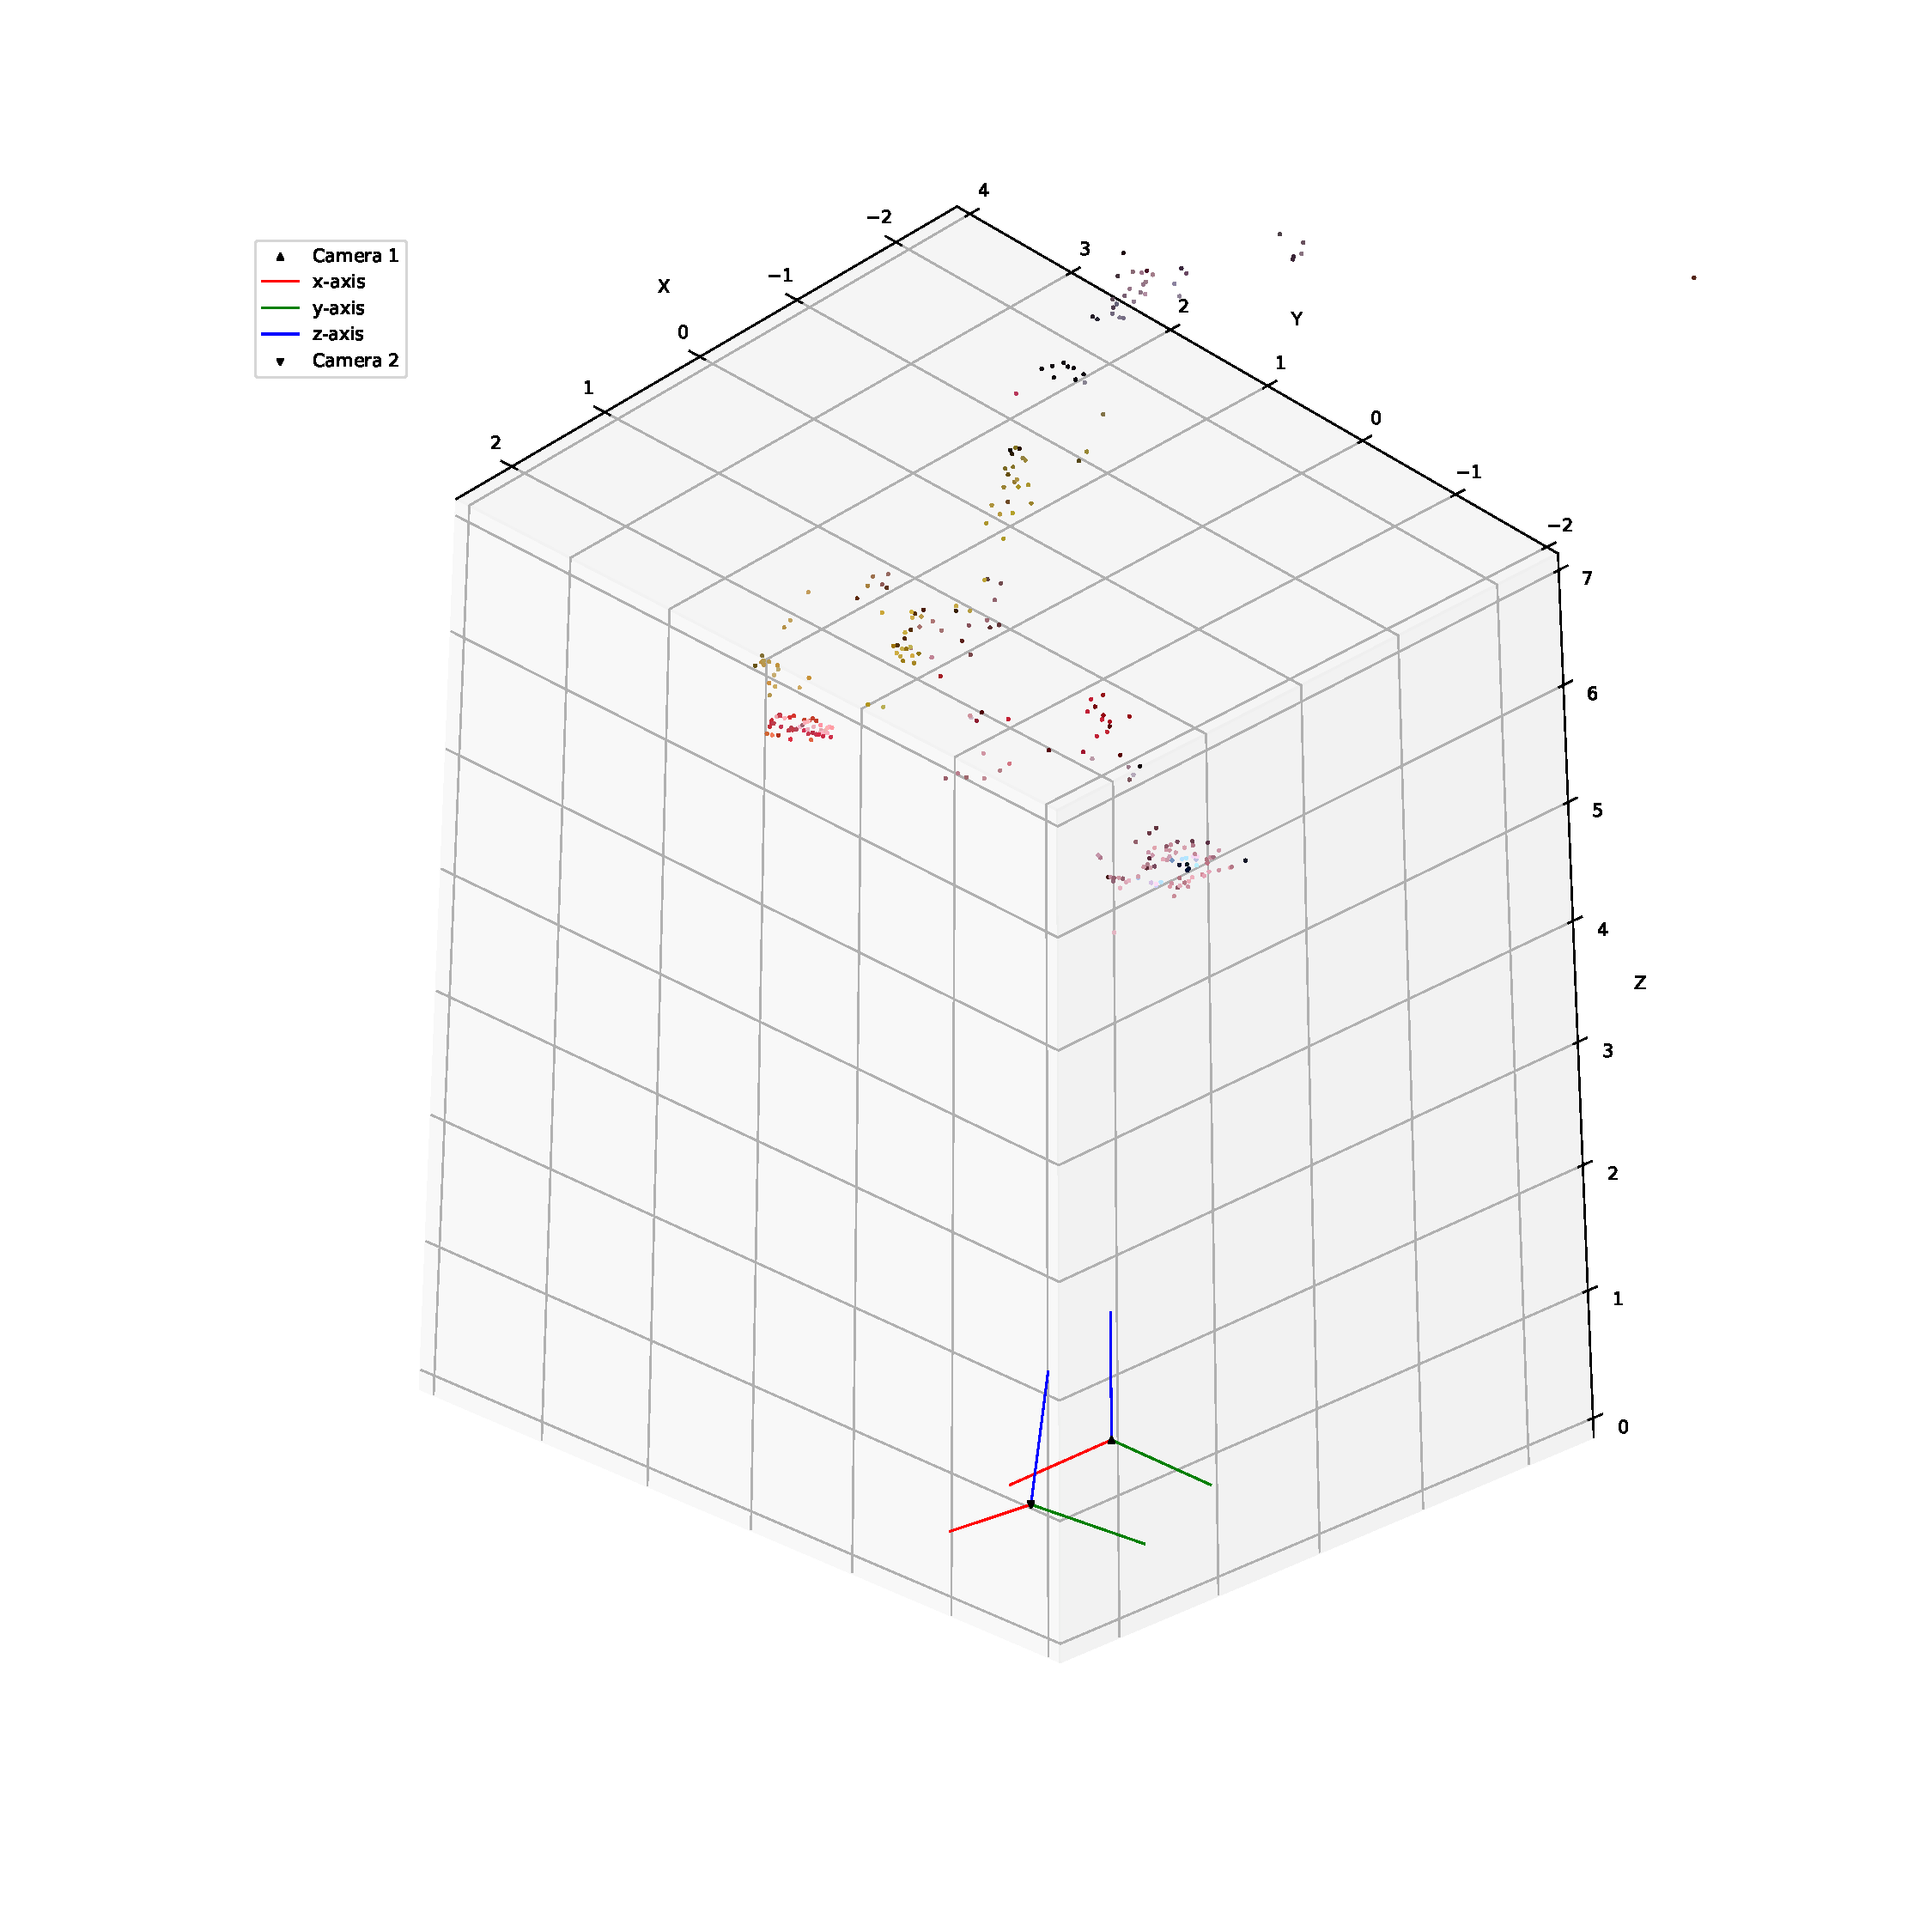
\includegraphics[width=\linewidth]{/home/madhia/computer_vision/assignment4/implementation/q1-2/output/et_3d_-30-135.pdf}
        \caption{Figure 2}
    \end{minipage}%
\end{figure}

\begin{figure}[h!]
    \centering
    \begin{minipage}{0.4\textwidth}
        \centering
        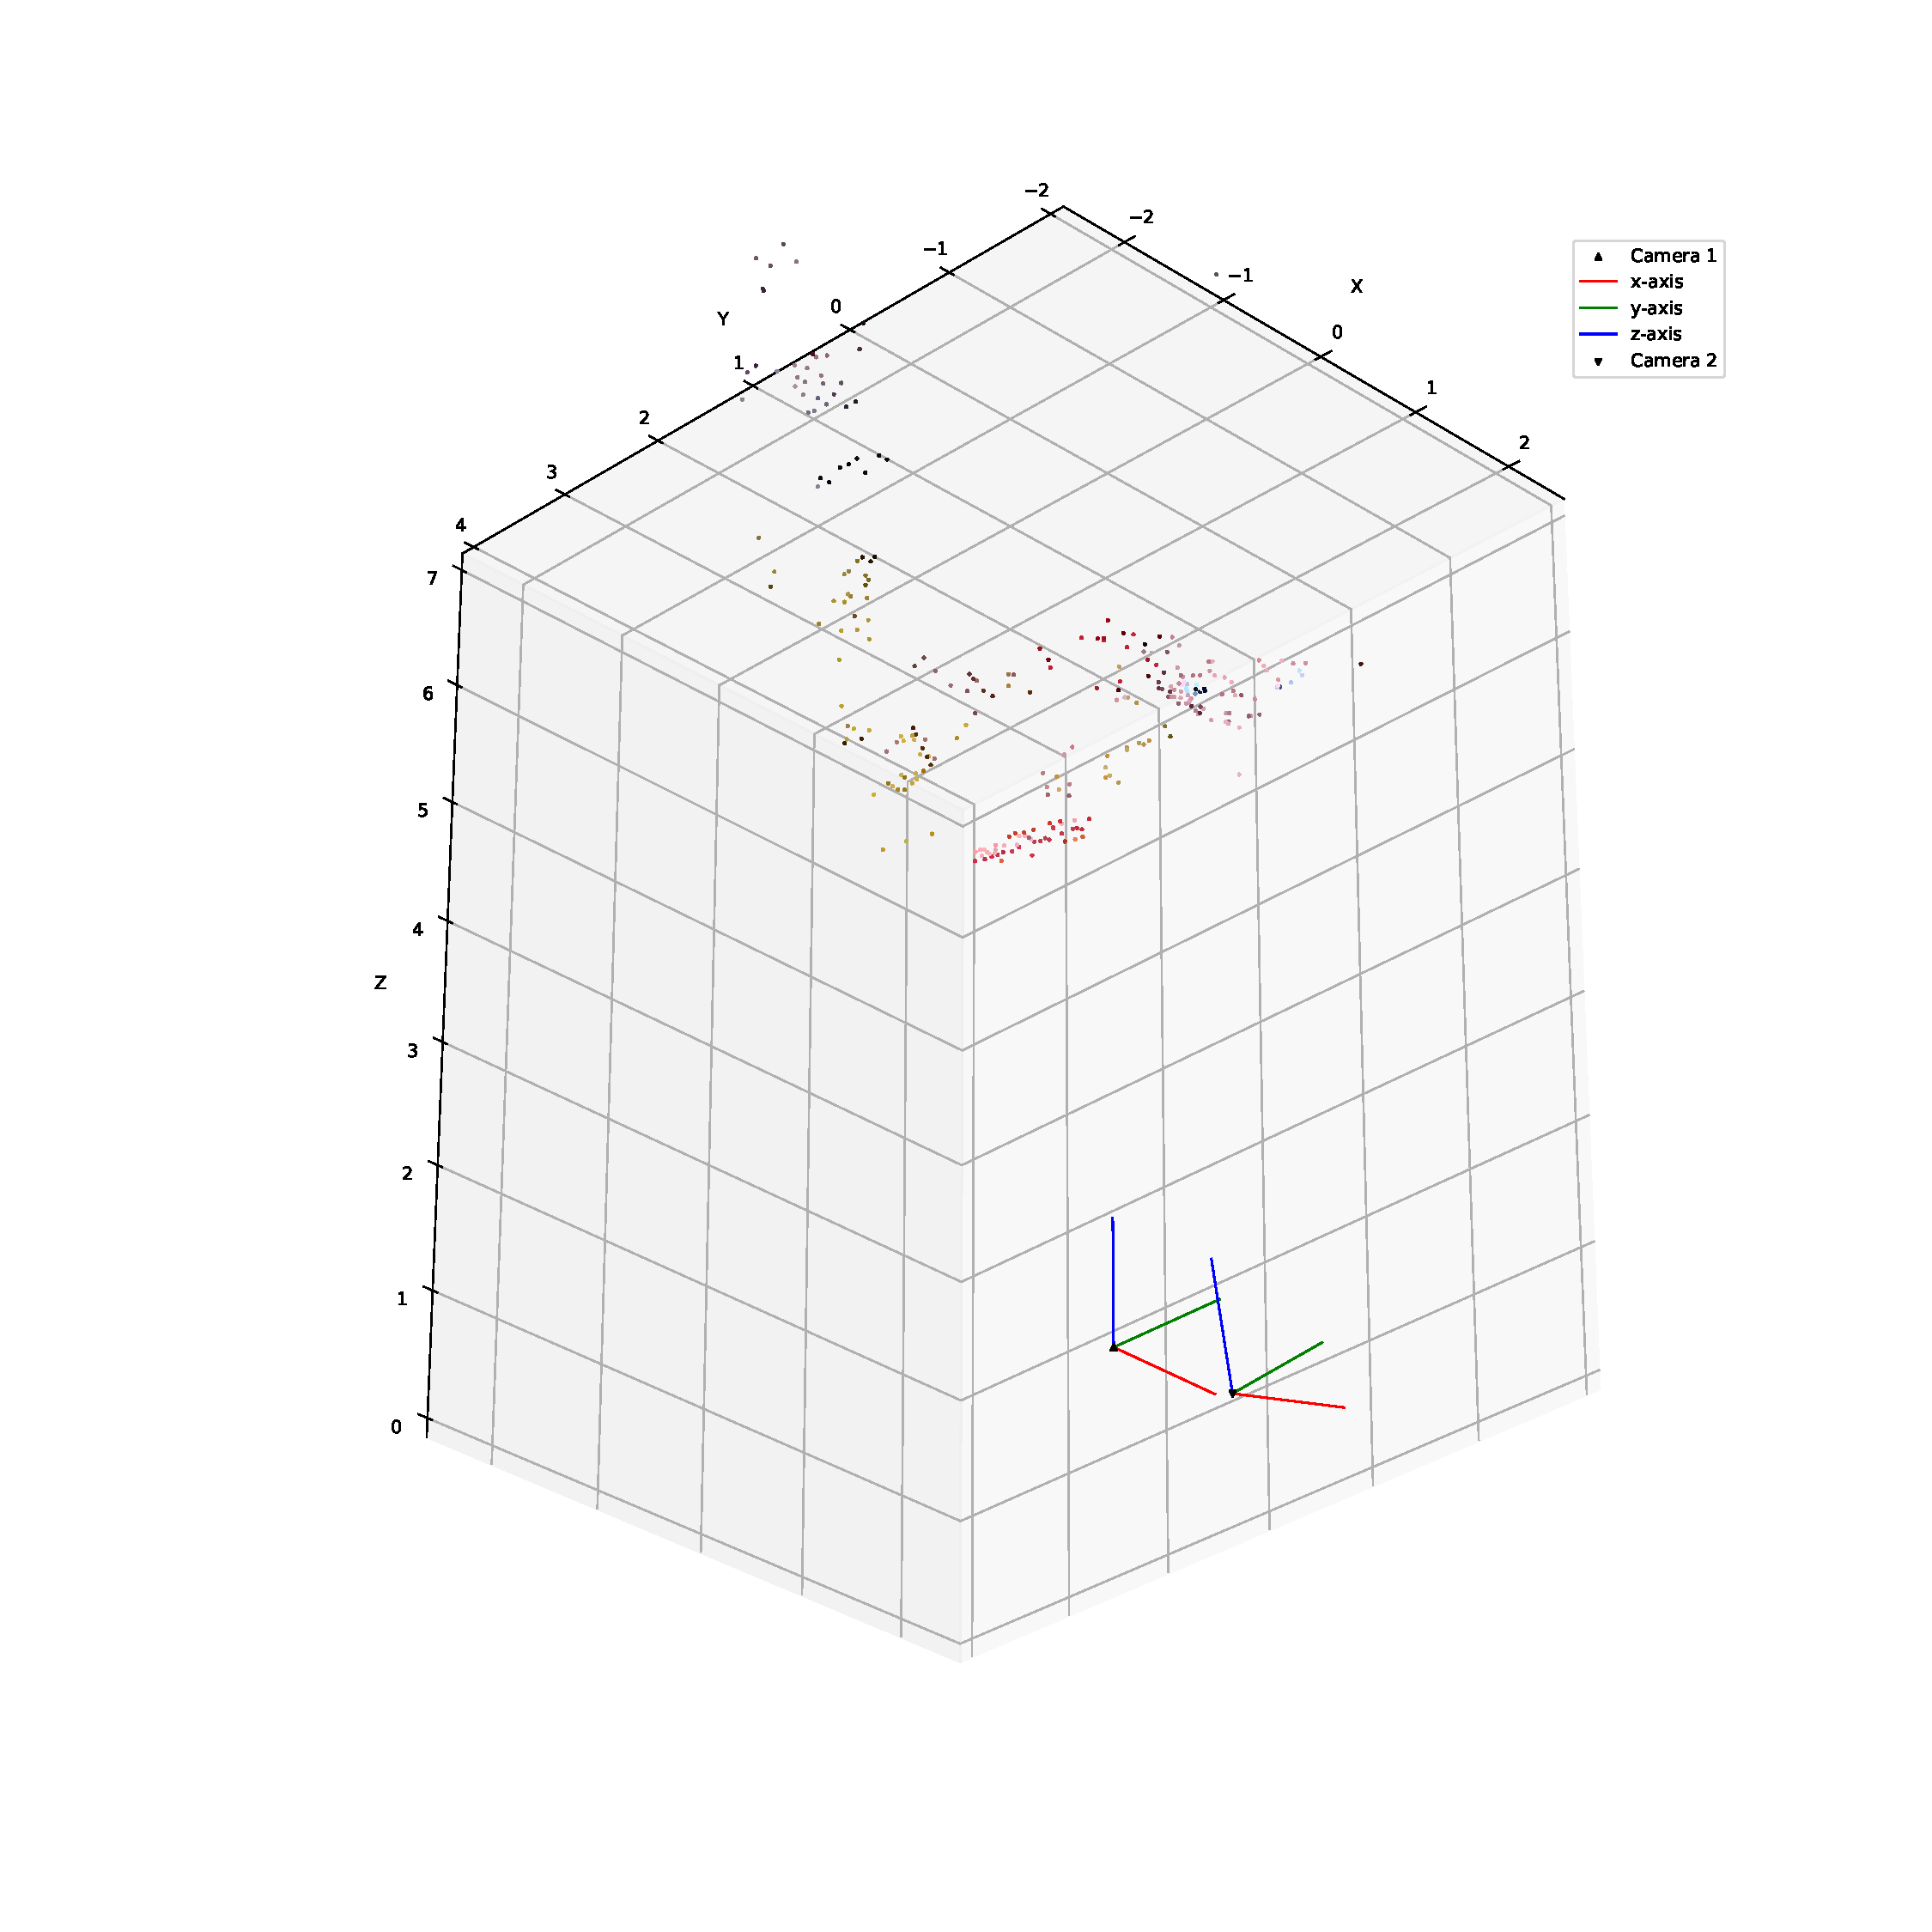
\includegraphics[width=\linewidth]{/home/madhia/computer_vision/assignment4/implementation/q1-2/output/et_3d_-30-225.pdf}
        \caption{Figure 3}
    \end{minipage}%
    \begin{minipage}{0.4\textwidth}
        \centering
        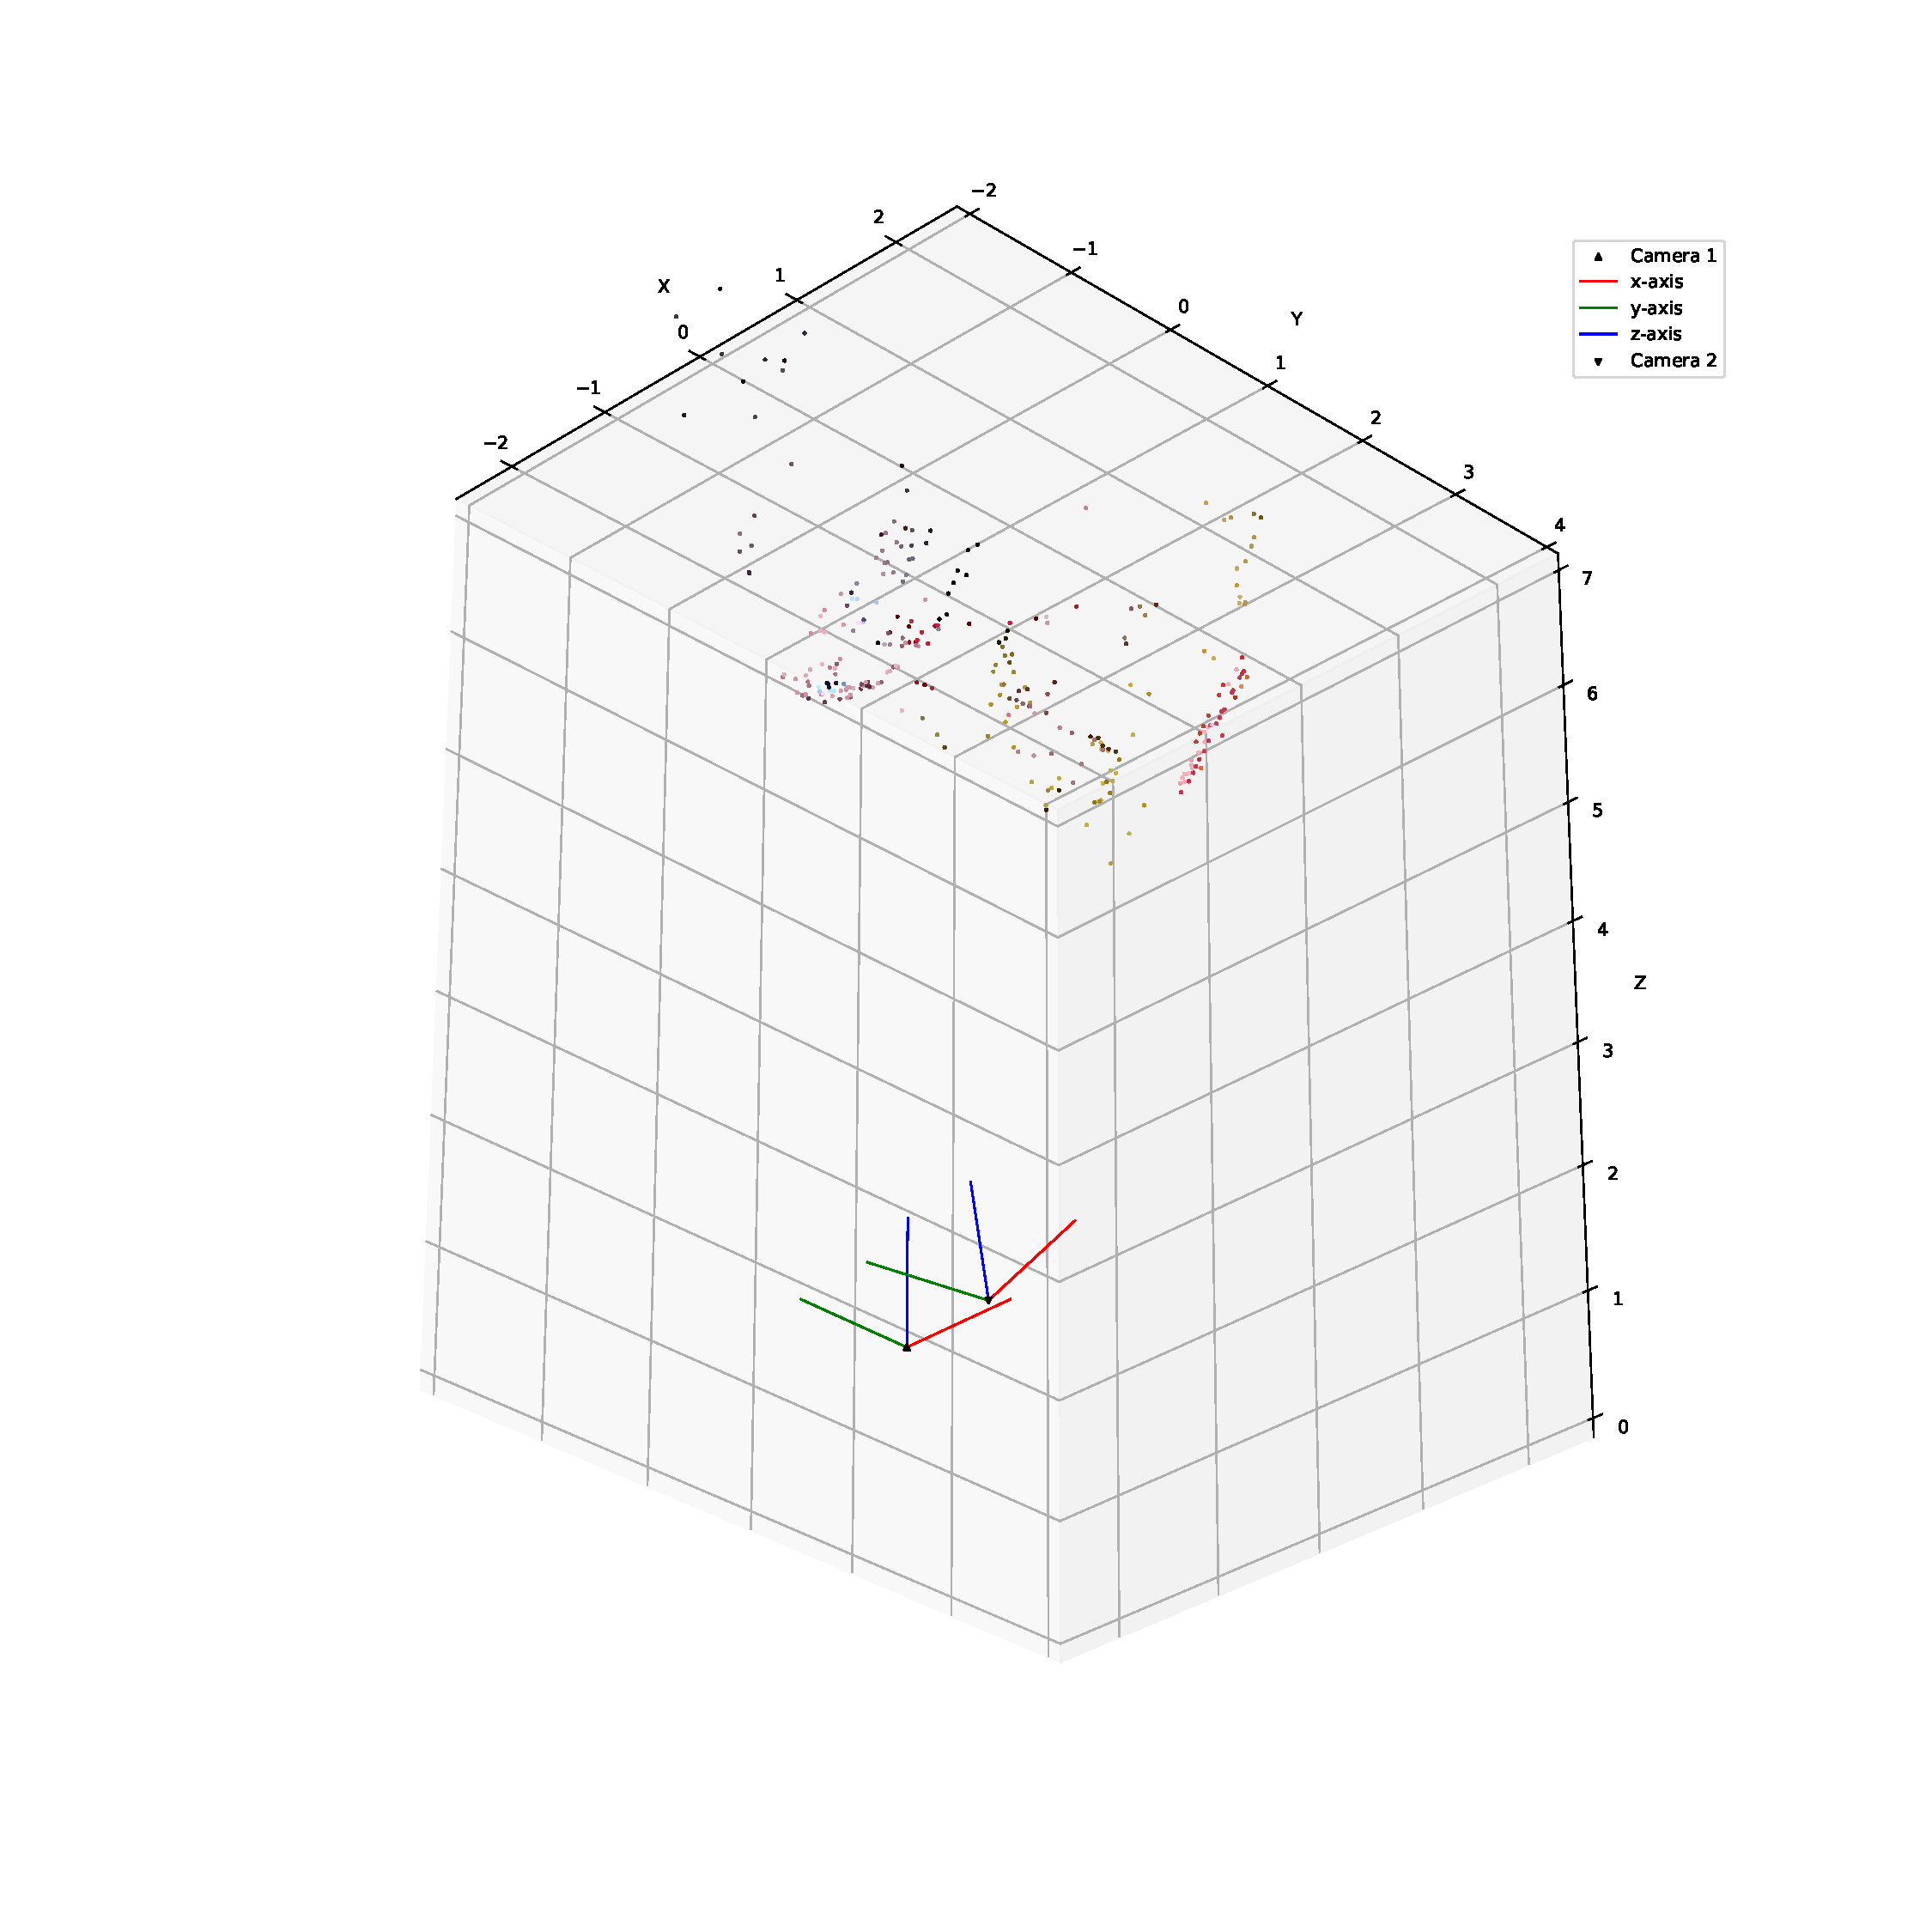
\includegraphics[width=\linewidth]{/home/madhia/computer_vision/assignment4/implementation/q1-2/output/et_3d_-30-315.pdf}
        \caption{Figure 4}
    \end{minipage}%
\end{figure}
    
\begin{figure}[h!]
    \centering    
    \begin{minipage}{0.4\textwidth}
        \centering
        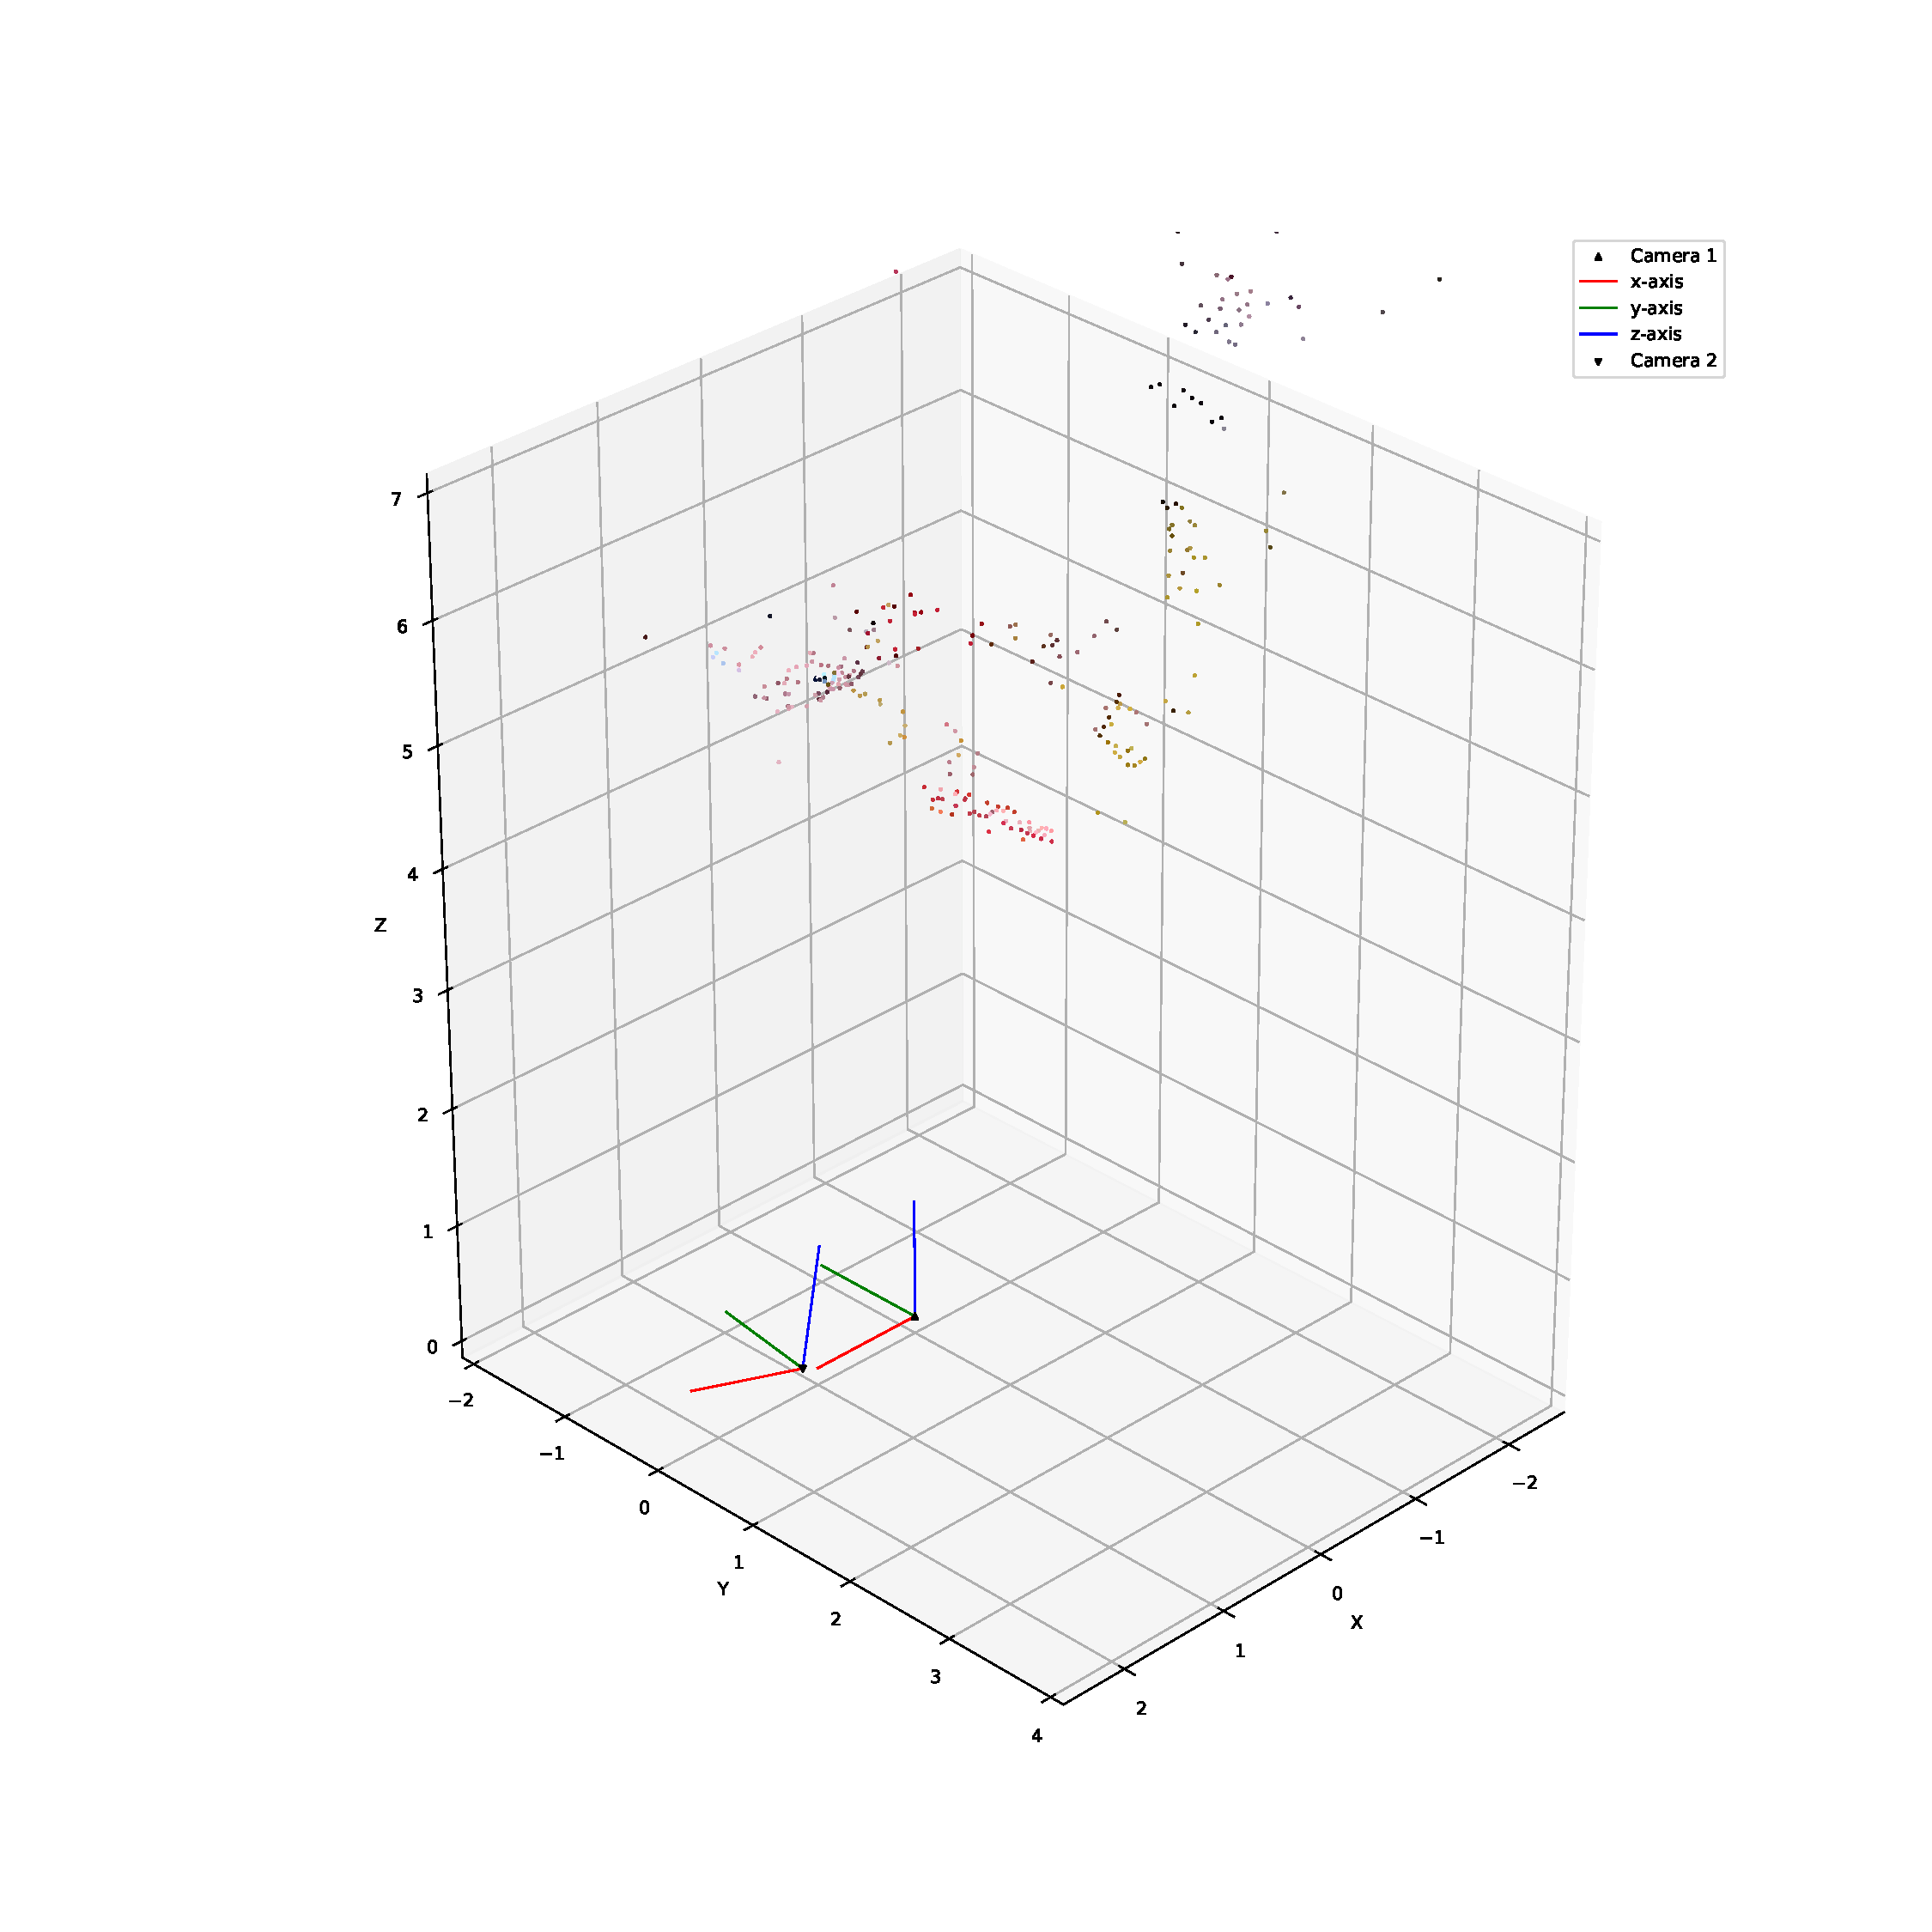
\includegraphics[width=\linewidth]{/home/madhia/computer_vision/assignment4/implementation/q1-2/output/et_3d_30-45.pdf}
        \caption{Figure 5}
    \end{minipage}%
    \begin{minipage}{0.4\textwidth}
        \centering
        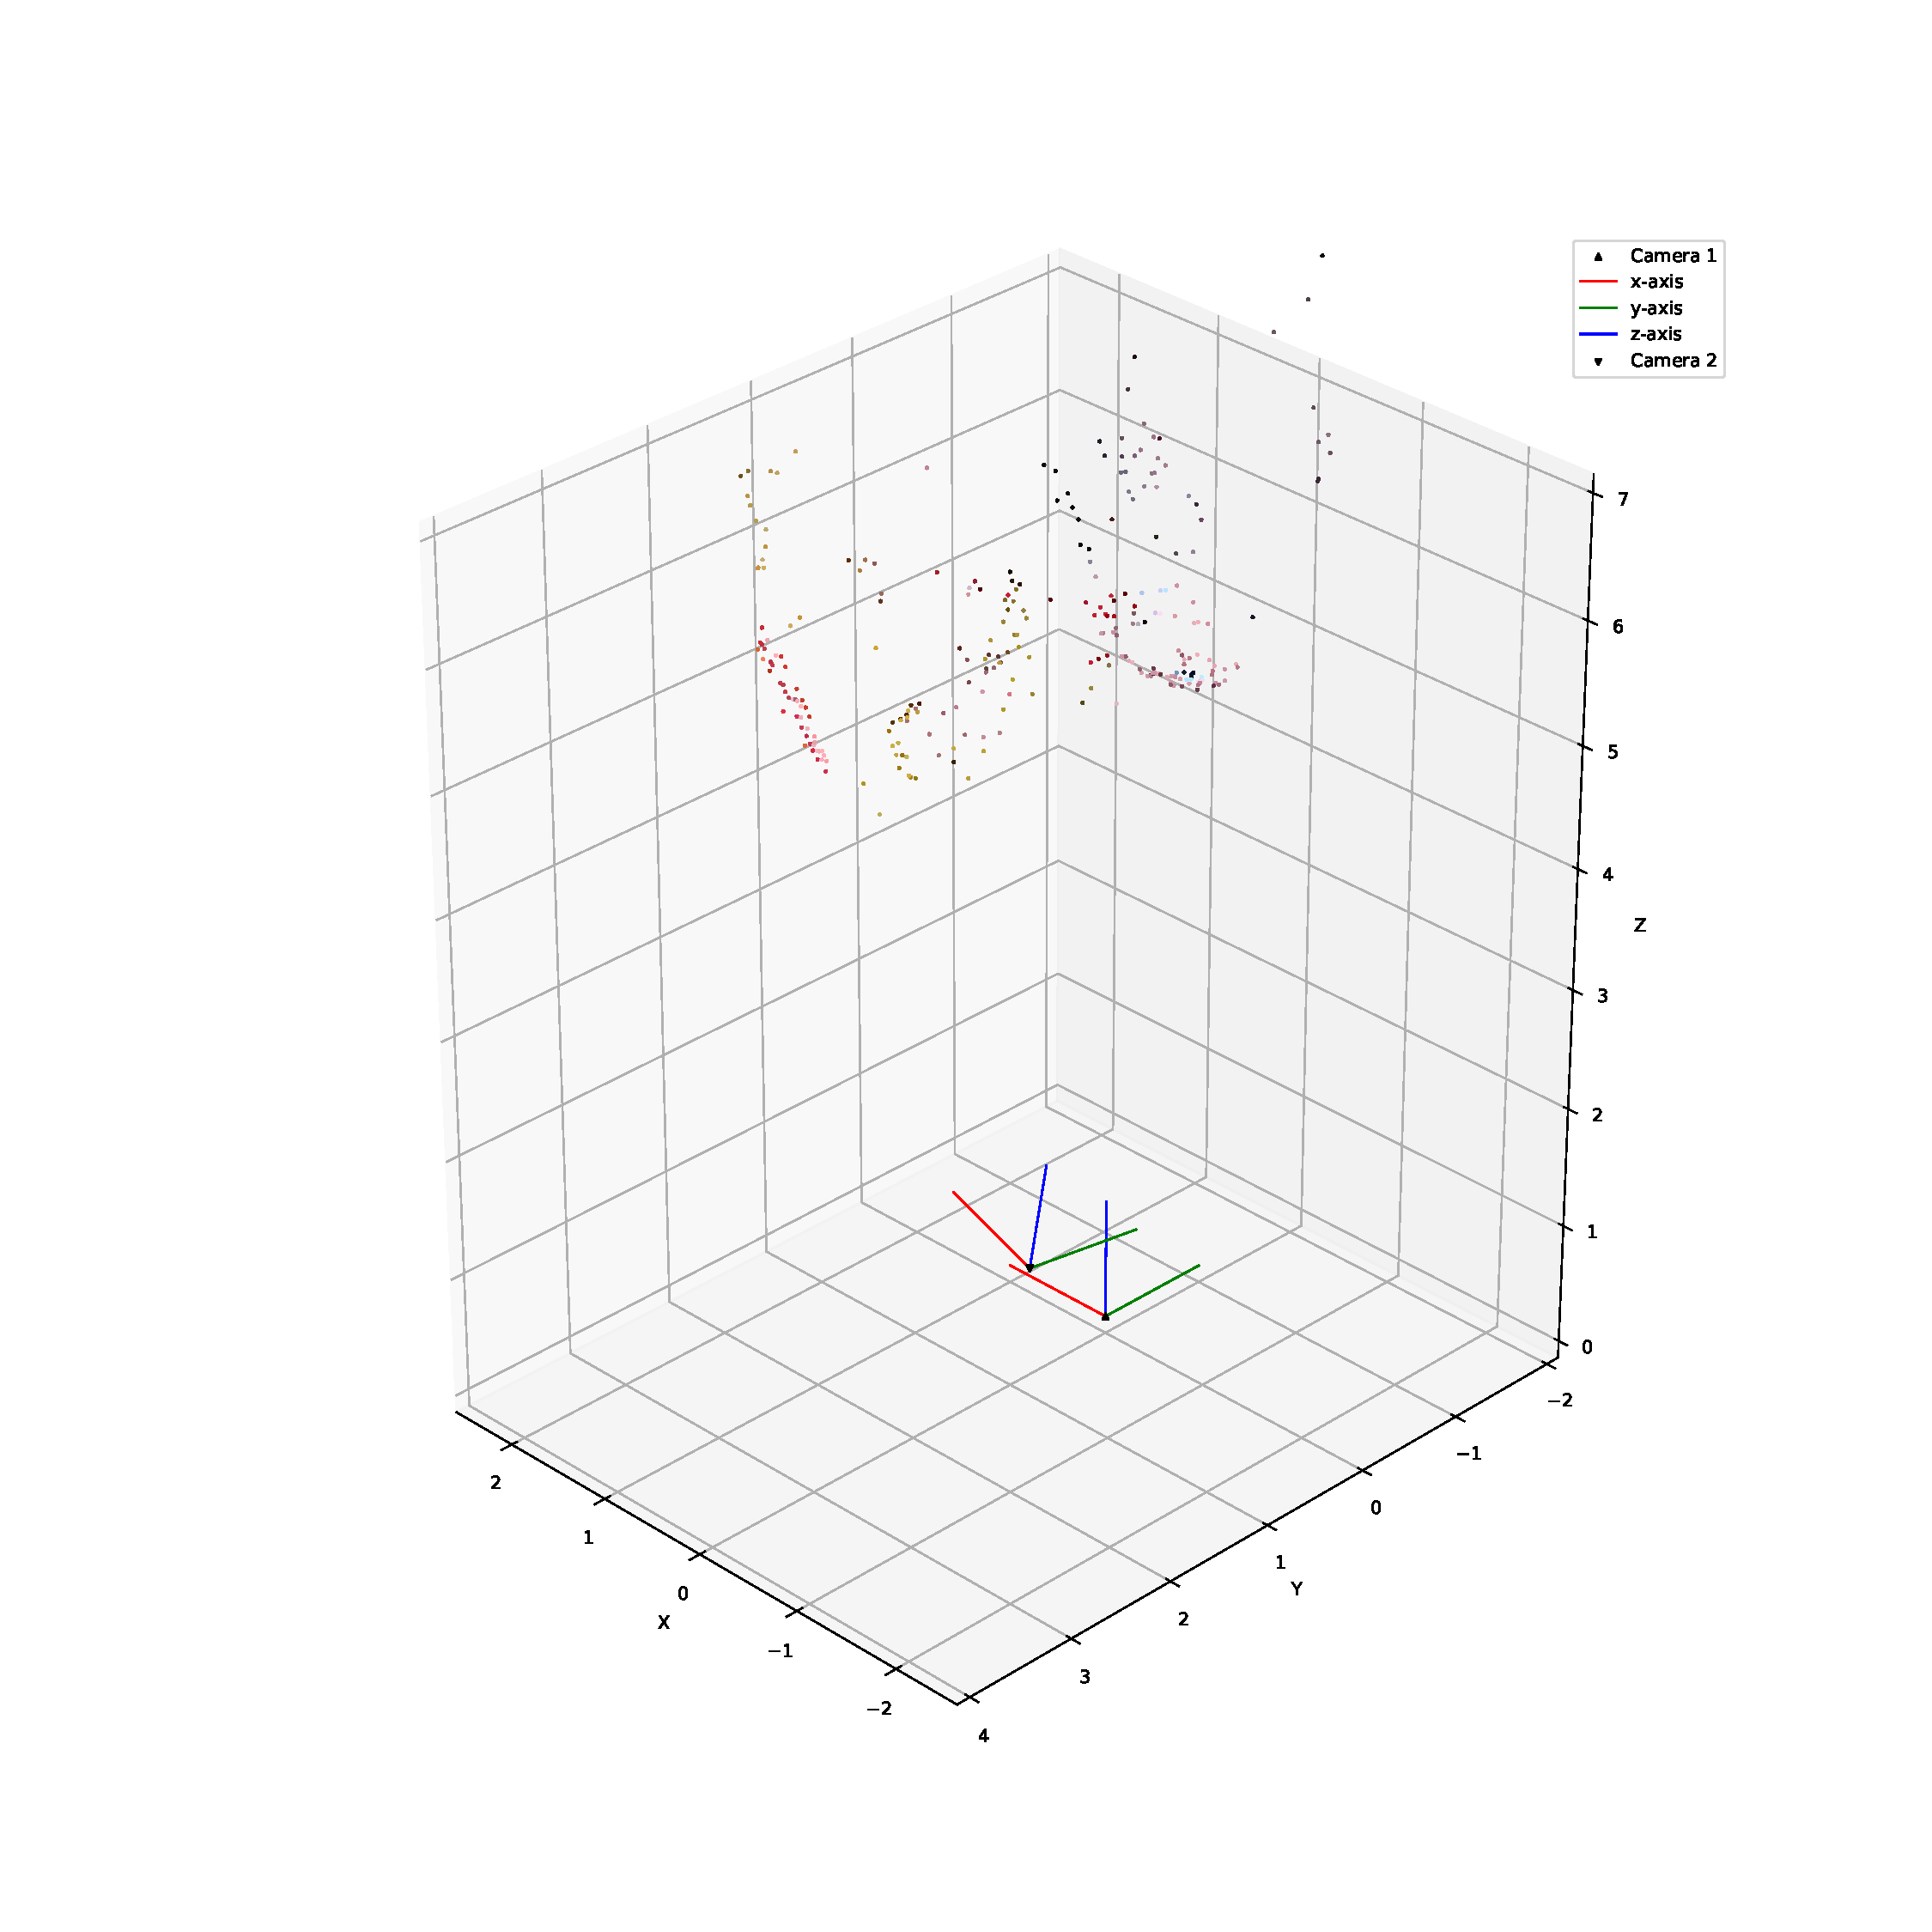
\includegraphics[width=\linewidth]{/home/madhia/computer_vision/assignment4/implementation/q1-2/output/et_3d_30-135.pdf}
        \caption{Figure 6}
    \end{minipage}%
\end{figure}
    
\begin{figure}[h!]
    \centering    
    \begin{minipage}{0.4\textwidth}
        \centering
        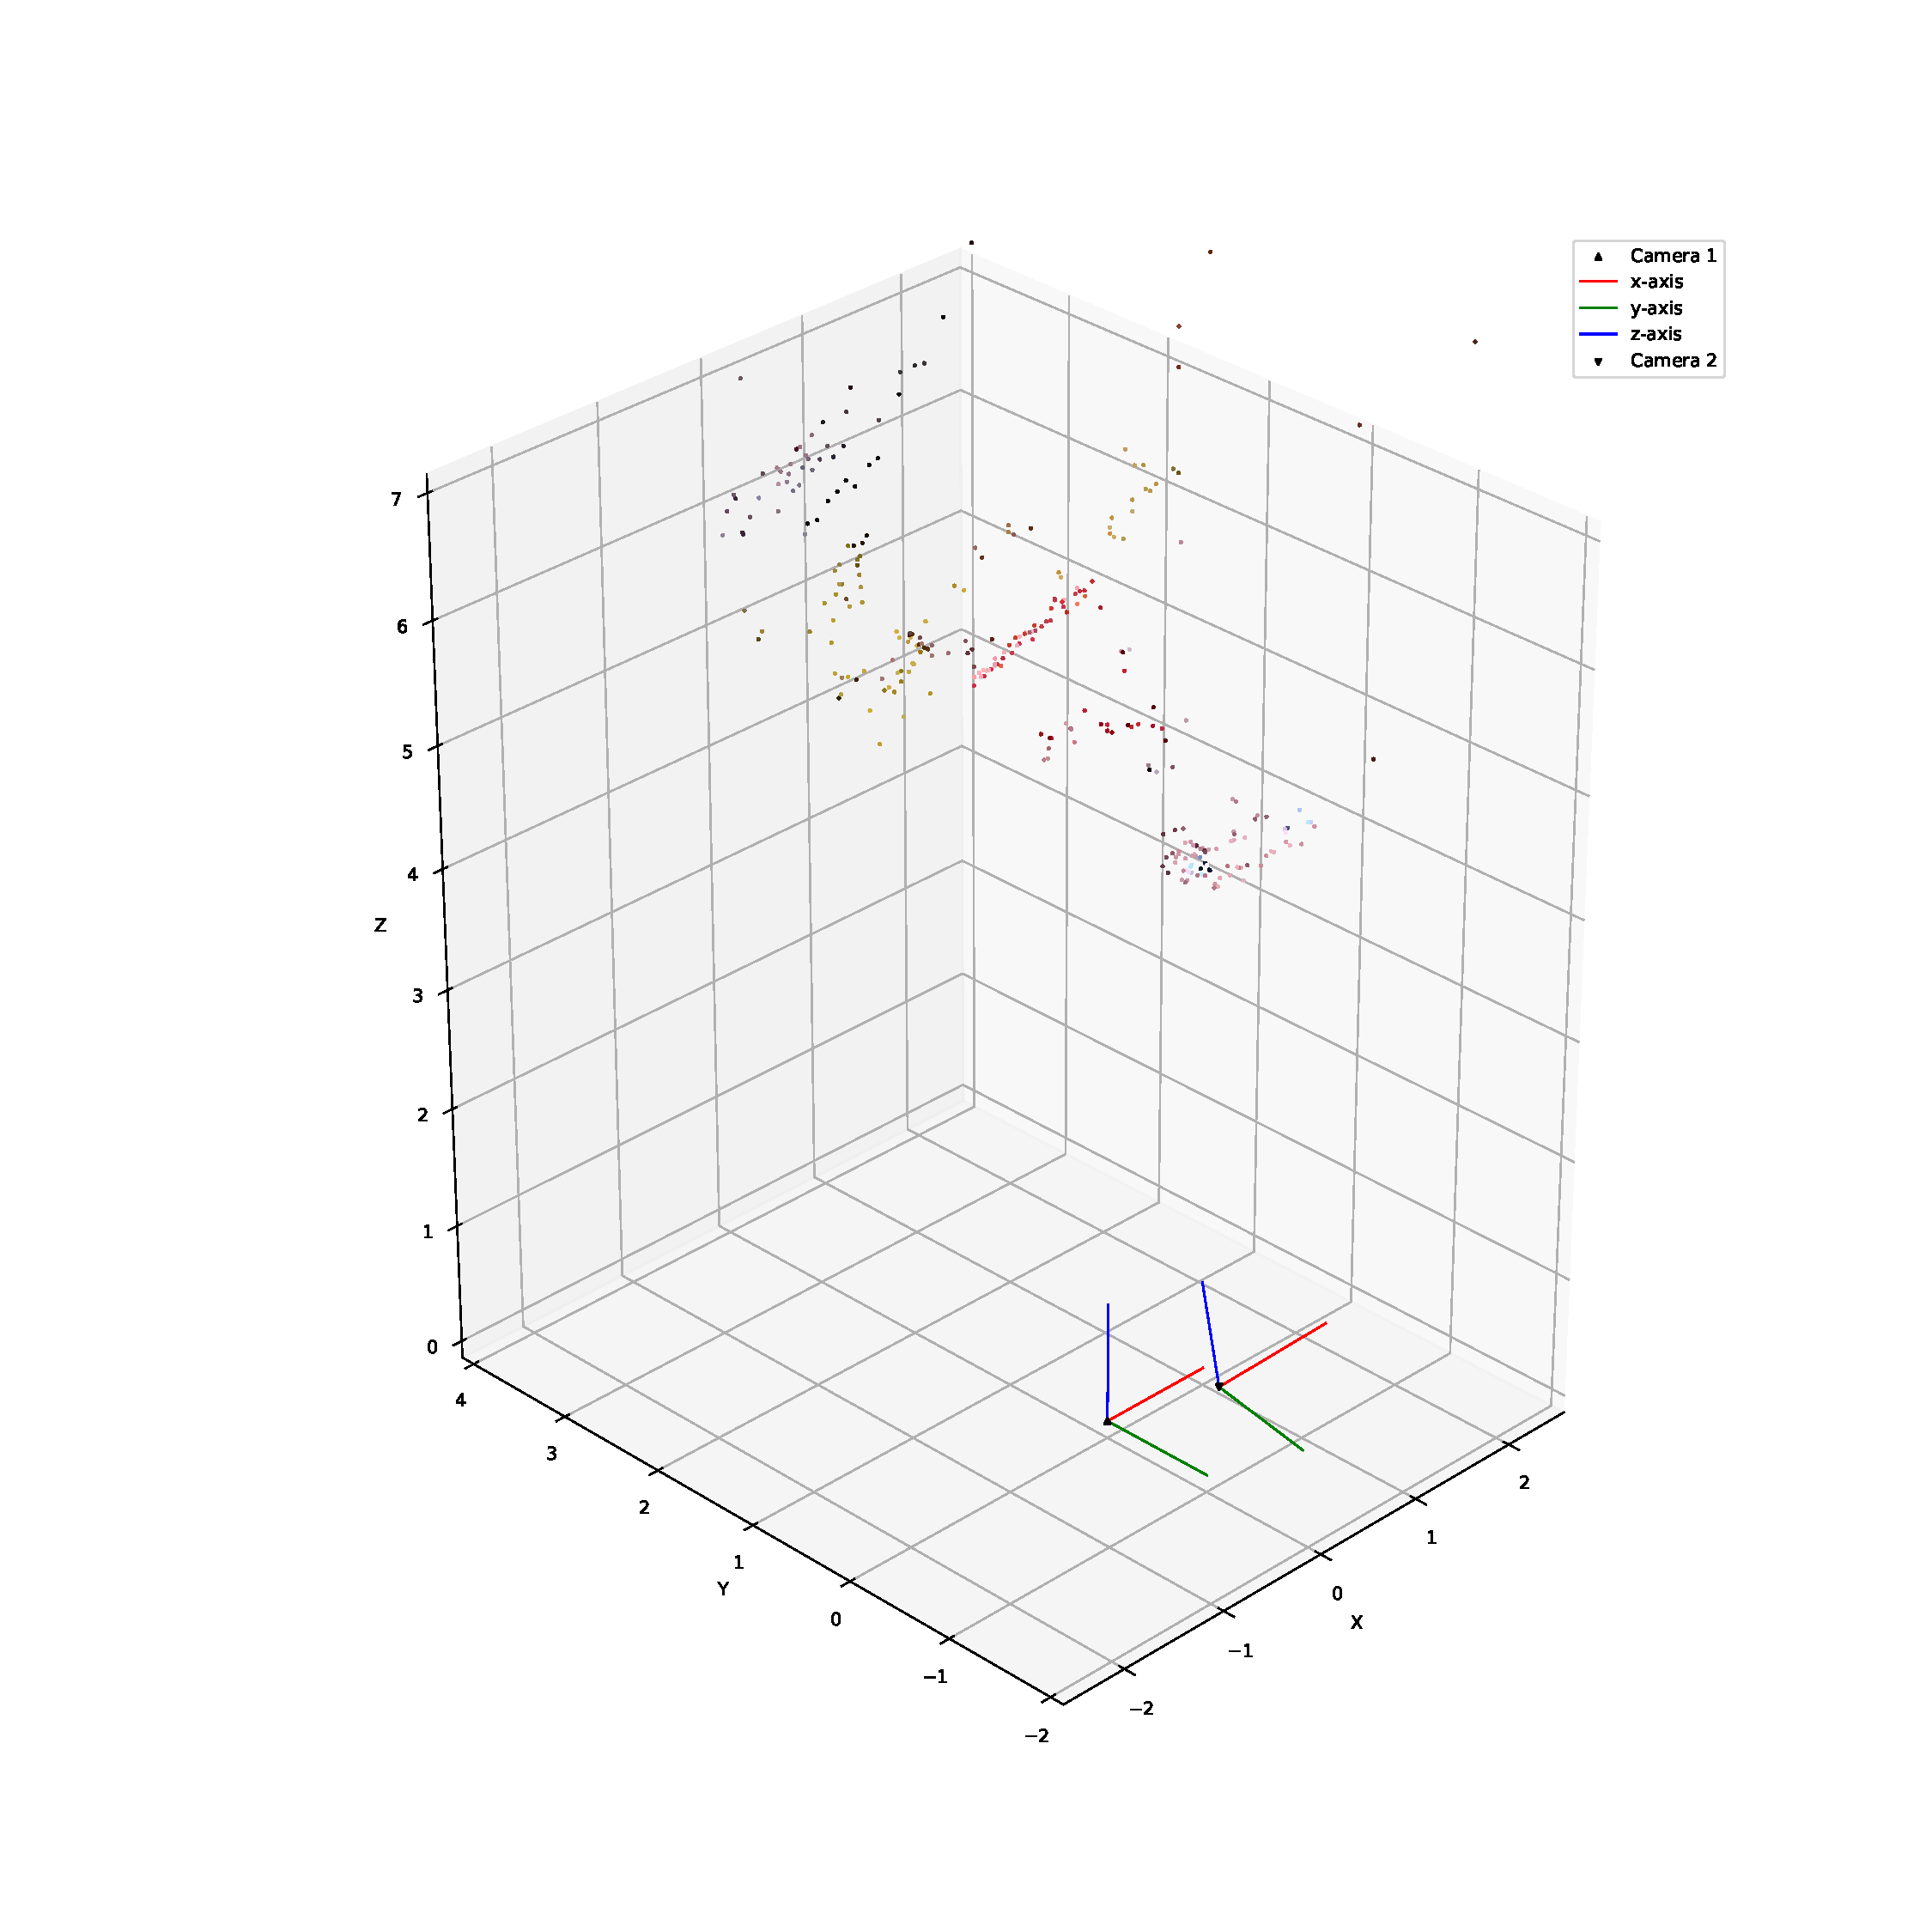
\includegraphics[width=\linewidth]{/home/madhia/computer_vision/assignment4/implementation/q1-2/output/et_3d_30-225.pdf}
        \caption{Figure 7}
    \end{minipage}%
    \begin{minipage}{0.4\textwidth}
        \centering
        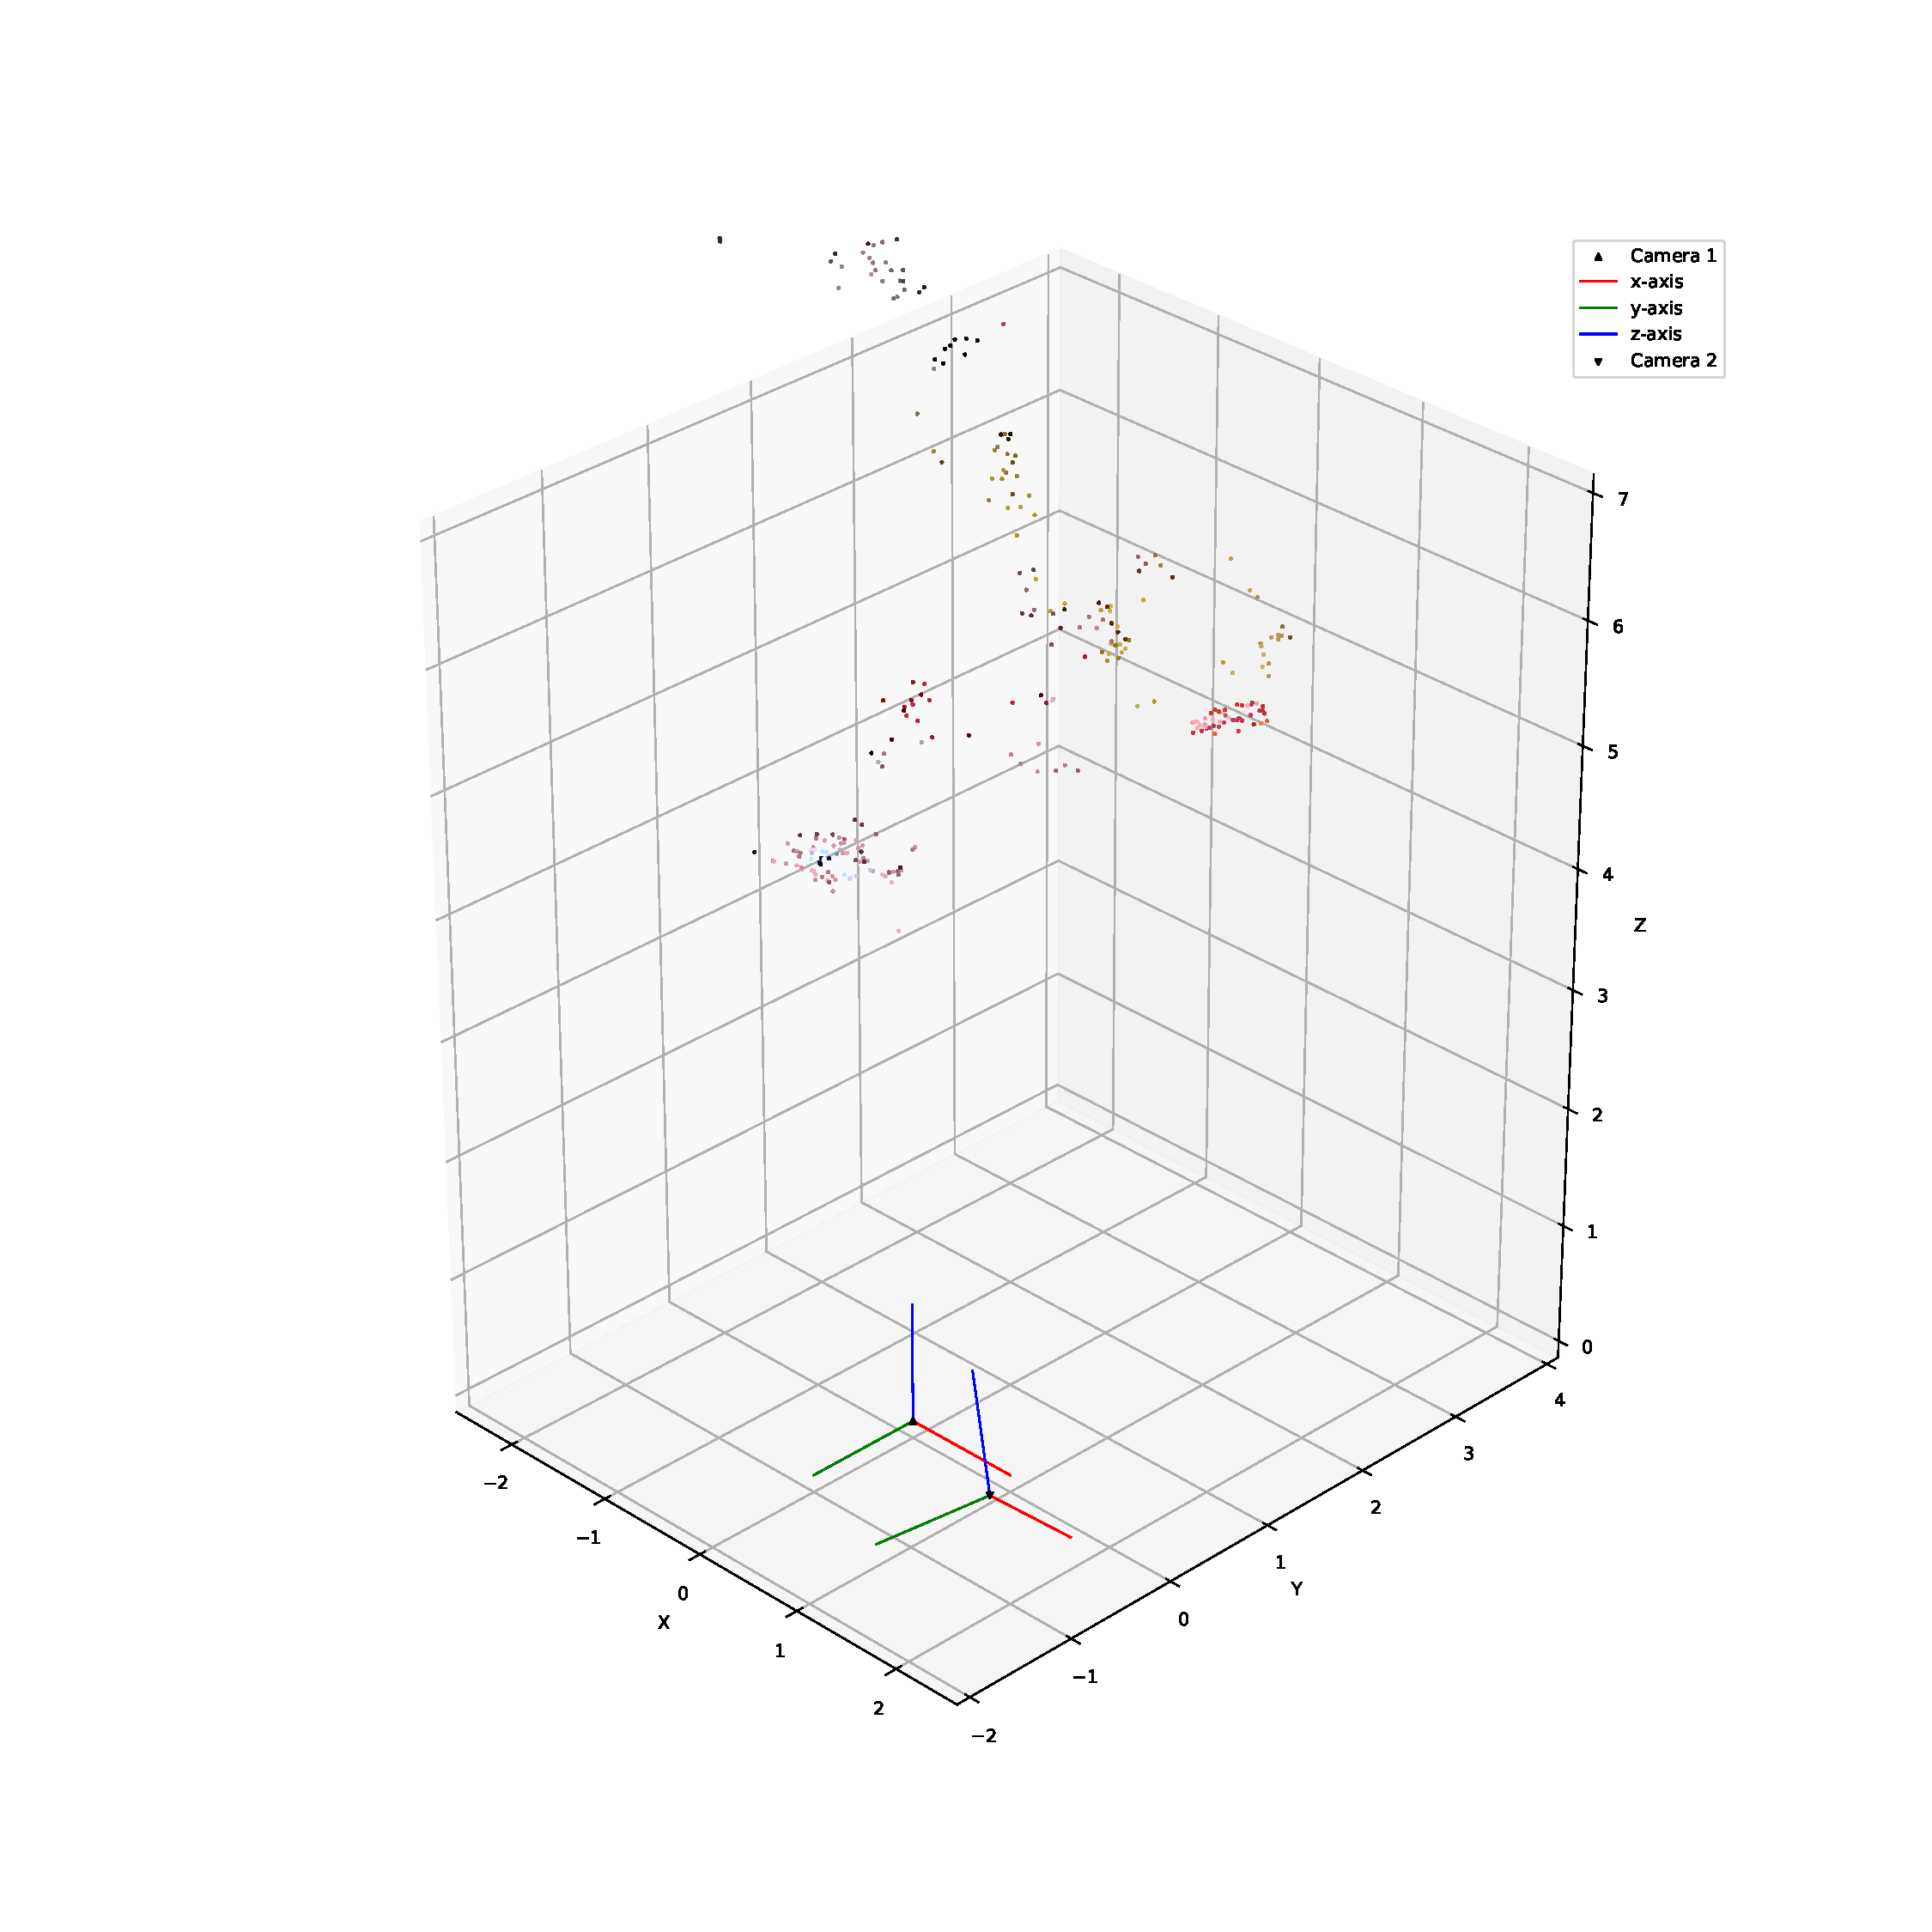
\includegraphics[width=\linewidth]{/home/madhia/computer_vision/assignment4/implementation/q1-2/output/et_3d_30-315.pdf}
        \caption{Figure 8}
    \end{minipage}
    \caption{Eight Figures Side by Side}
\end{figure}


\textbf{Discussion}: Discuss any challenges with the reconstruction, such as inaccuracies with points far from the cameras.

\section{Rectifying an Image Pair}

\subsection{Problem Description}
Describe the process of rectifying an image pair using the camera matrices obtained in the previous section.

\textbf{Aim}: Align the two images such that matching points have the same vertical coordinates.

\subsection{Part (a): Image Rectification}
\textbf{Description}: Explain how the camera matrices were used to rectify the images.

\textbf{Results}: Present the rectified images.

\begin{figure}[h!]
    \centering    
    \begin{minipage}{0.4\textwidth}
        \centering
        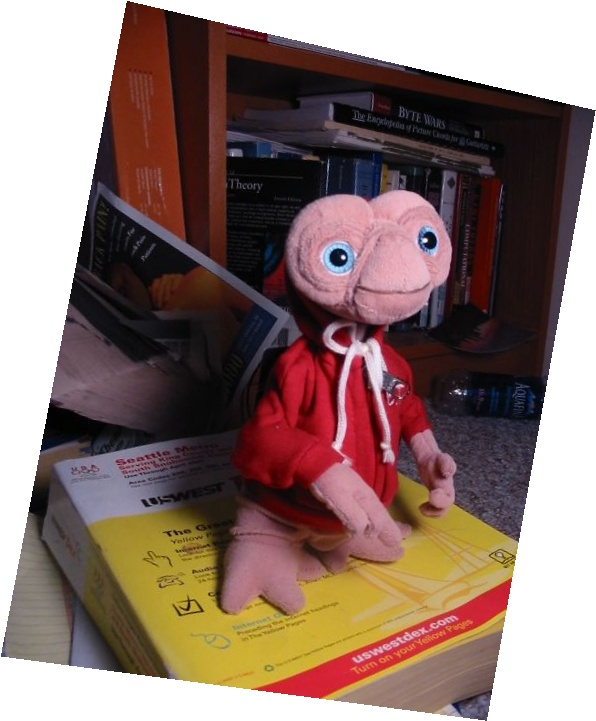
\includegraphics[width=\linewidth]{/home/madhia/computer_vision/assignment4/implementation/q1-2/output/et1_t.jpg}
        \caption{Figure 7}
    \end{minipage}%
    \begin{minipage}{0.4\textwidth}
        \centering
        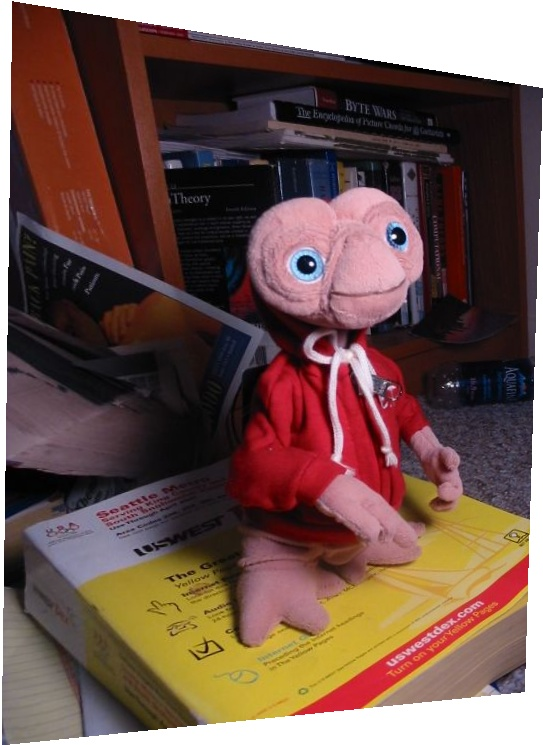
\includegraphics[width=\linewidth]{/home/madhia/computer_vision/assignment4/implementation/q1-2/output/et2_t.jpg}
        \caption{Figure 8}
    \end{minipage}
    \caption{Eight Figures Side by Side}
\end{figure}

\textbf{Discussion}: Discuss any challenges encountered during rectification, such as changes to the image coordinate system.

\subsection{Part (b): Drawing Epipolar Lines}
\textbf{Description}: Explain how epipolar lines were drawn on the rectified images.

\textbf{Results}: Show images with epipolar lines.

% \begin{figure}[h!]
%     \centering
%     \includegraphics[width=0.8\textwidth]{epipolar_lines.png}
%     \caption{Epipolar lines on rectified images.}
% \end{figure}

\textbf{Discussion}: Discuss why epipolar lines should be horizontal in rectified images and any challenges in ensuring alignment.

\section{Verifying Solutions on Another Dataset}
\subsection{Problem Description}
Describe how the methods were applied to the "fountain" dataset. Briefly discuss any changes made.

\subsection{Results}

\textit{Fundamental Matrix $\mathbf{F}$}
\[
\mathbf{F} = \begin{bmatrix} 
-6.83743697 \times 10^{-9} & 1.25824306 \times 10^{-7} & -1.81029773 \times 10^{-4} \\ 
.33230570 \times 10^{-7} & 1.74654927 \times 10^{-8} & 2.79790329 \times 10^{-3} \\ 
-2.98233372 \times 10^{-4} & -3.65851022 \times 10^{-3} & 1 
\end{bmatrix}
\]

\textit{Essential Matrix $\mathbf{E}$}
\[
\mathbf{E} = \begin{bmatrix}
-0.0520653 & 0.95974592 & -0.17866541 \\ 
2.54177187 & 0.13344791 & 9.18319912 \\ 
0.07414608 & -9.53523233 & 0.10944801 
\end{bmatrix}
\]

\textit{Matrix $\mathbf{U}$}
\[
\mathbf{U} = \begin{bmatrix}
-0.10155205 & 0.00955263 & 0.99478436 \\ 
0.0836553 & -0.99633022 & 0.01810739 \\ 
0.9913067 & 0.08505783 & 0.10038025 
\end{bmatrix}
\]

\textit{Singular Values (S)}
\[
\mathbf{S} = \begin{bmatrix}
9.58495513 & 0 & 0 \\ 
0 & 9.53058587 & 0 \\ 
0 & 0 & 1.73688159 \times 10^{-3} 
\end{bmatrix}
\]

\textit{Matrix $\mathbf{V}^T$}
\[
\mathbf{V}^T = \begin{bmatrix}
0.03040406 & -0.99516796 & 0.09336128 \\ 
-0.26510802 & -0.09808801 & -0.9592166 \\ 
0.96373924 & 0.00441325 & -0.26680928 
\end{bmatrix}
\]

\textit{Projection Matrix $\mathbf{P}$}
\[
\mathbf{P} = \begin{bmatrix}
2.75948162 \times 10^{3} & 6.03317758 \times 10^{-4} & 1.52069460 \times 10^{3} & 0 \\ 
0 & 2.76416669 \times 10^{3} & 1.00681246 \times 10^{3} & 0 \\ 
0 & 0 & 1.00000033 & 0 
\end{bmatrix}
\]

\textit{Projection Matrix $\mathbf{P}'$}
\[
\mathbf{P}' = \begin{bmatrix}
3.12274904 \times 10^{3} & -2.17879605 \times 10^{1} & 4.18586484 \times 10^{2} & 2.89773688 \times 10^{3} \\ 
3.90403121 \times 10^{2} & 2.77673801 \times 10^{3} & 8.89719196 \times 10^{2} & 1.51115913 \times 10^{2} \\ 
3.62129963 \times 10^{-1} & 1.30314881 \times 10^{-2} & 9.32036867 \times 10^{-1} & 1.00380278 \times 10^{-1} 
\end{bmatrix}
\]

\begin{figure}[h!]
    \centering
    \begin{minipage}{0.4\textwidth}
        \centering
        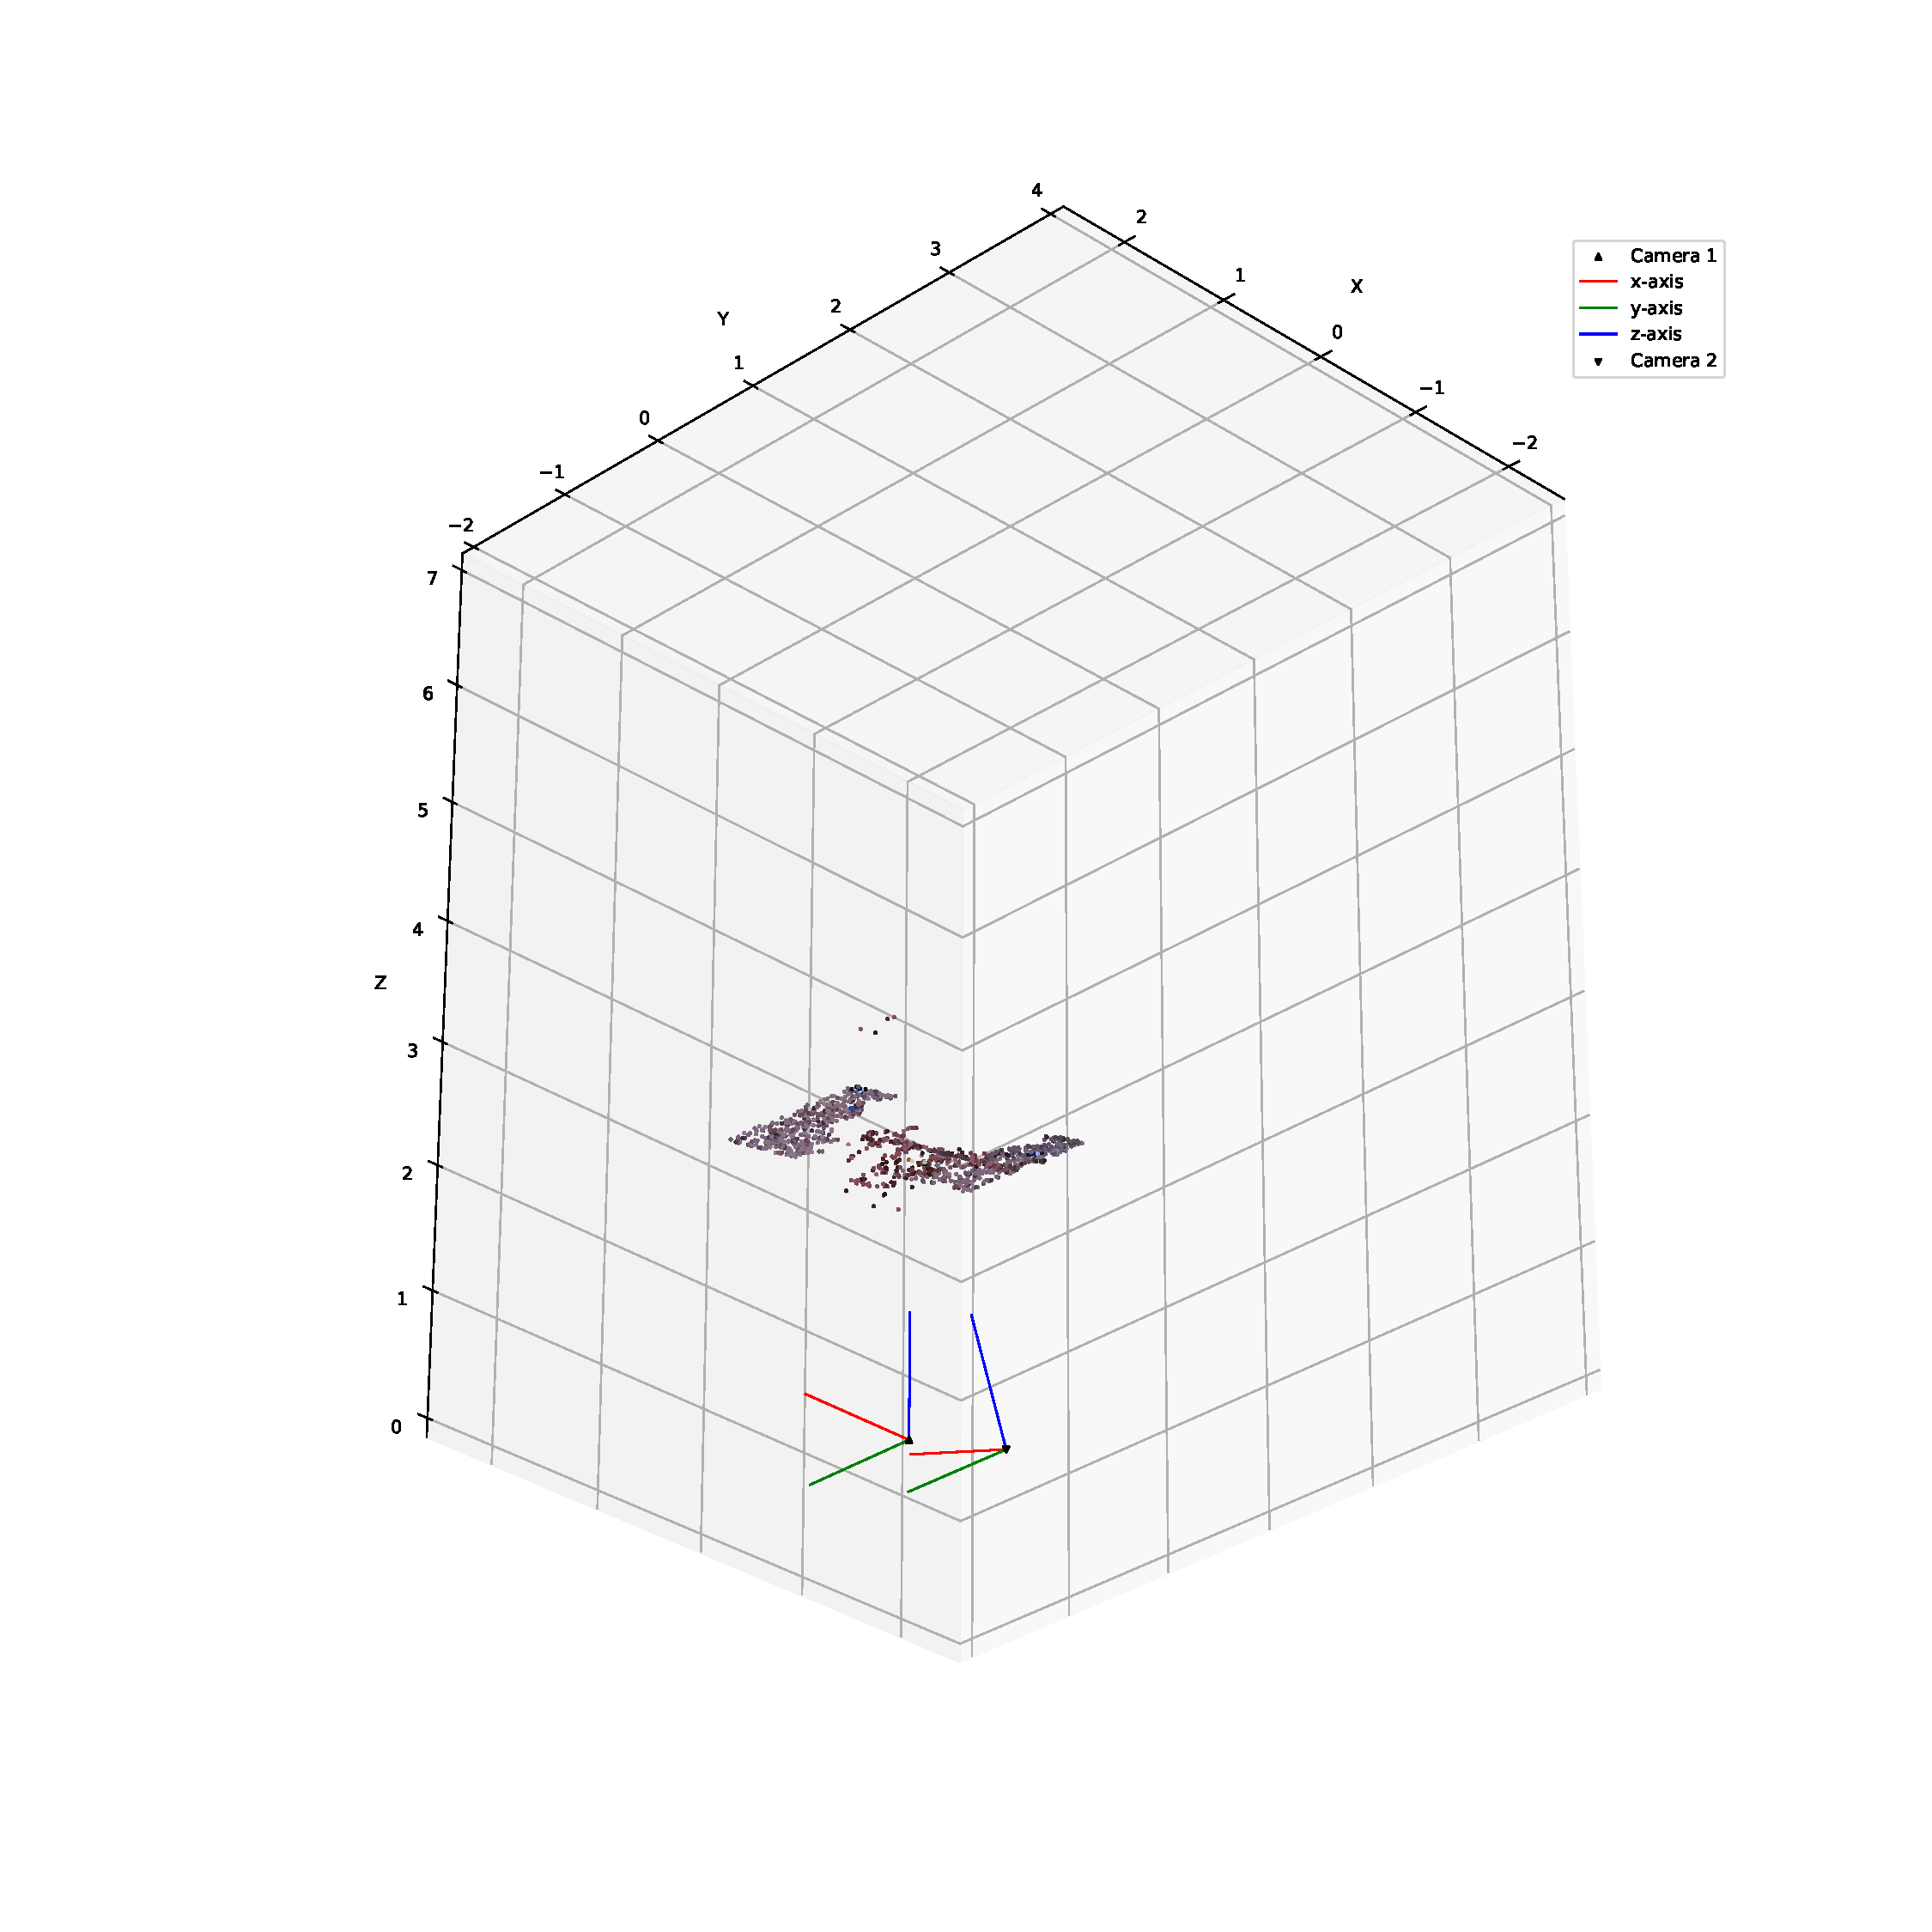
\includegraphics[width=\linewidth]{/home/madhia/computer_vision/assignment4/implementation/q3/output/fountain_3d_-30-45.pdf}
        \caption{Figure 1}
    \end{minipage}%
    \begin{minipage}{0.4\textwidth}
        \centering
        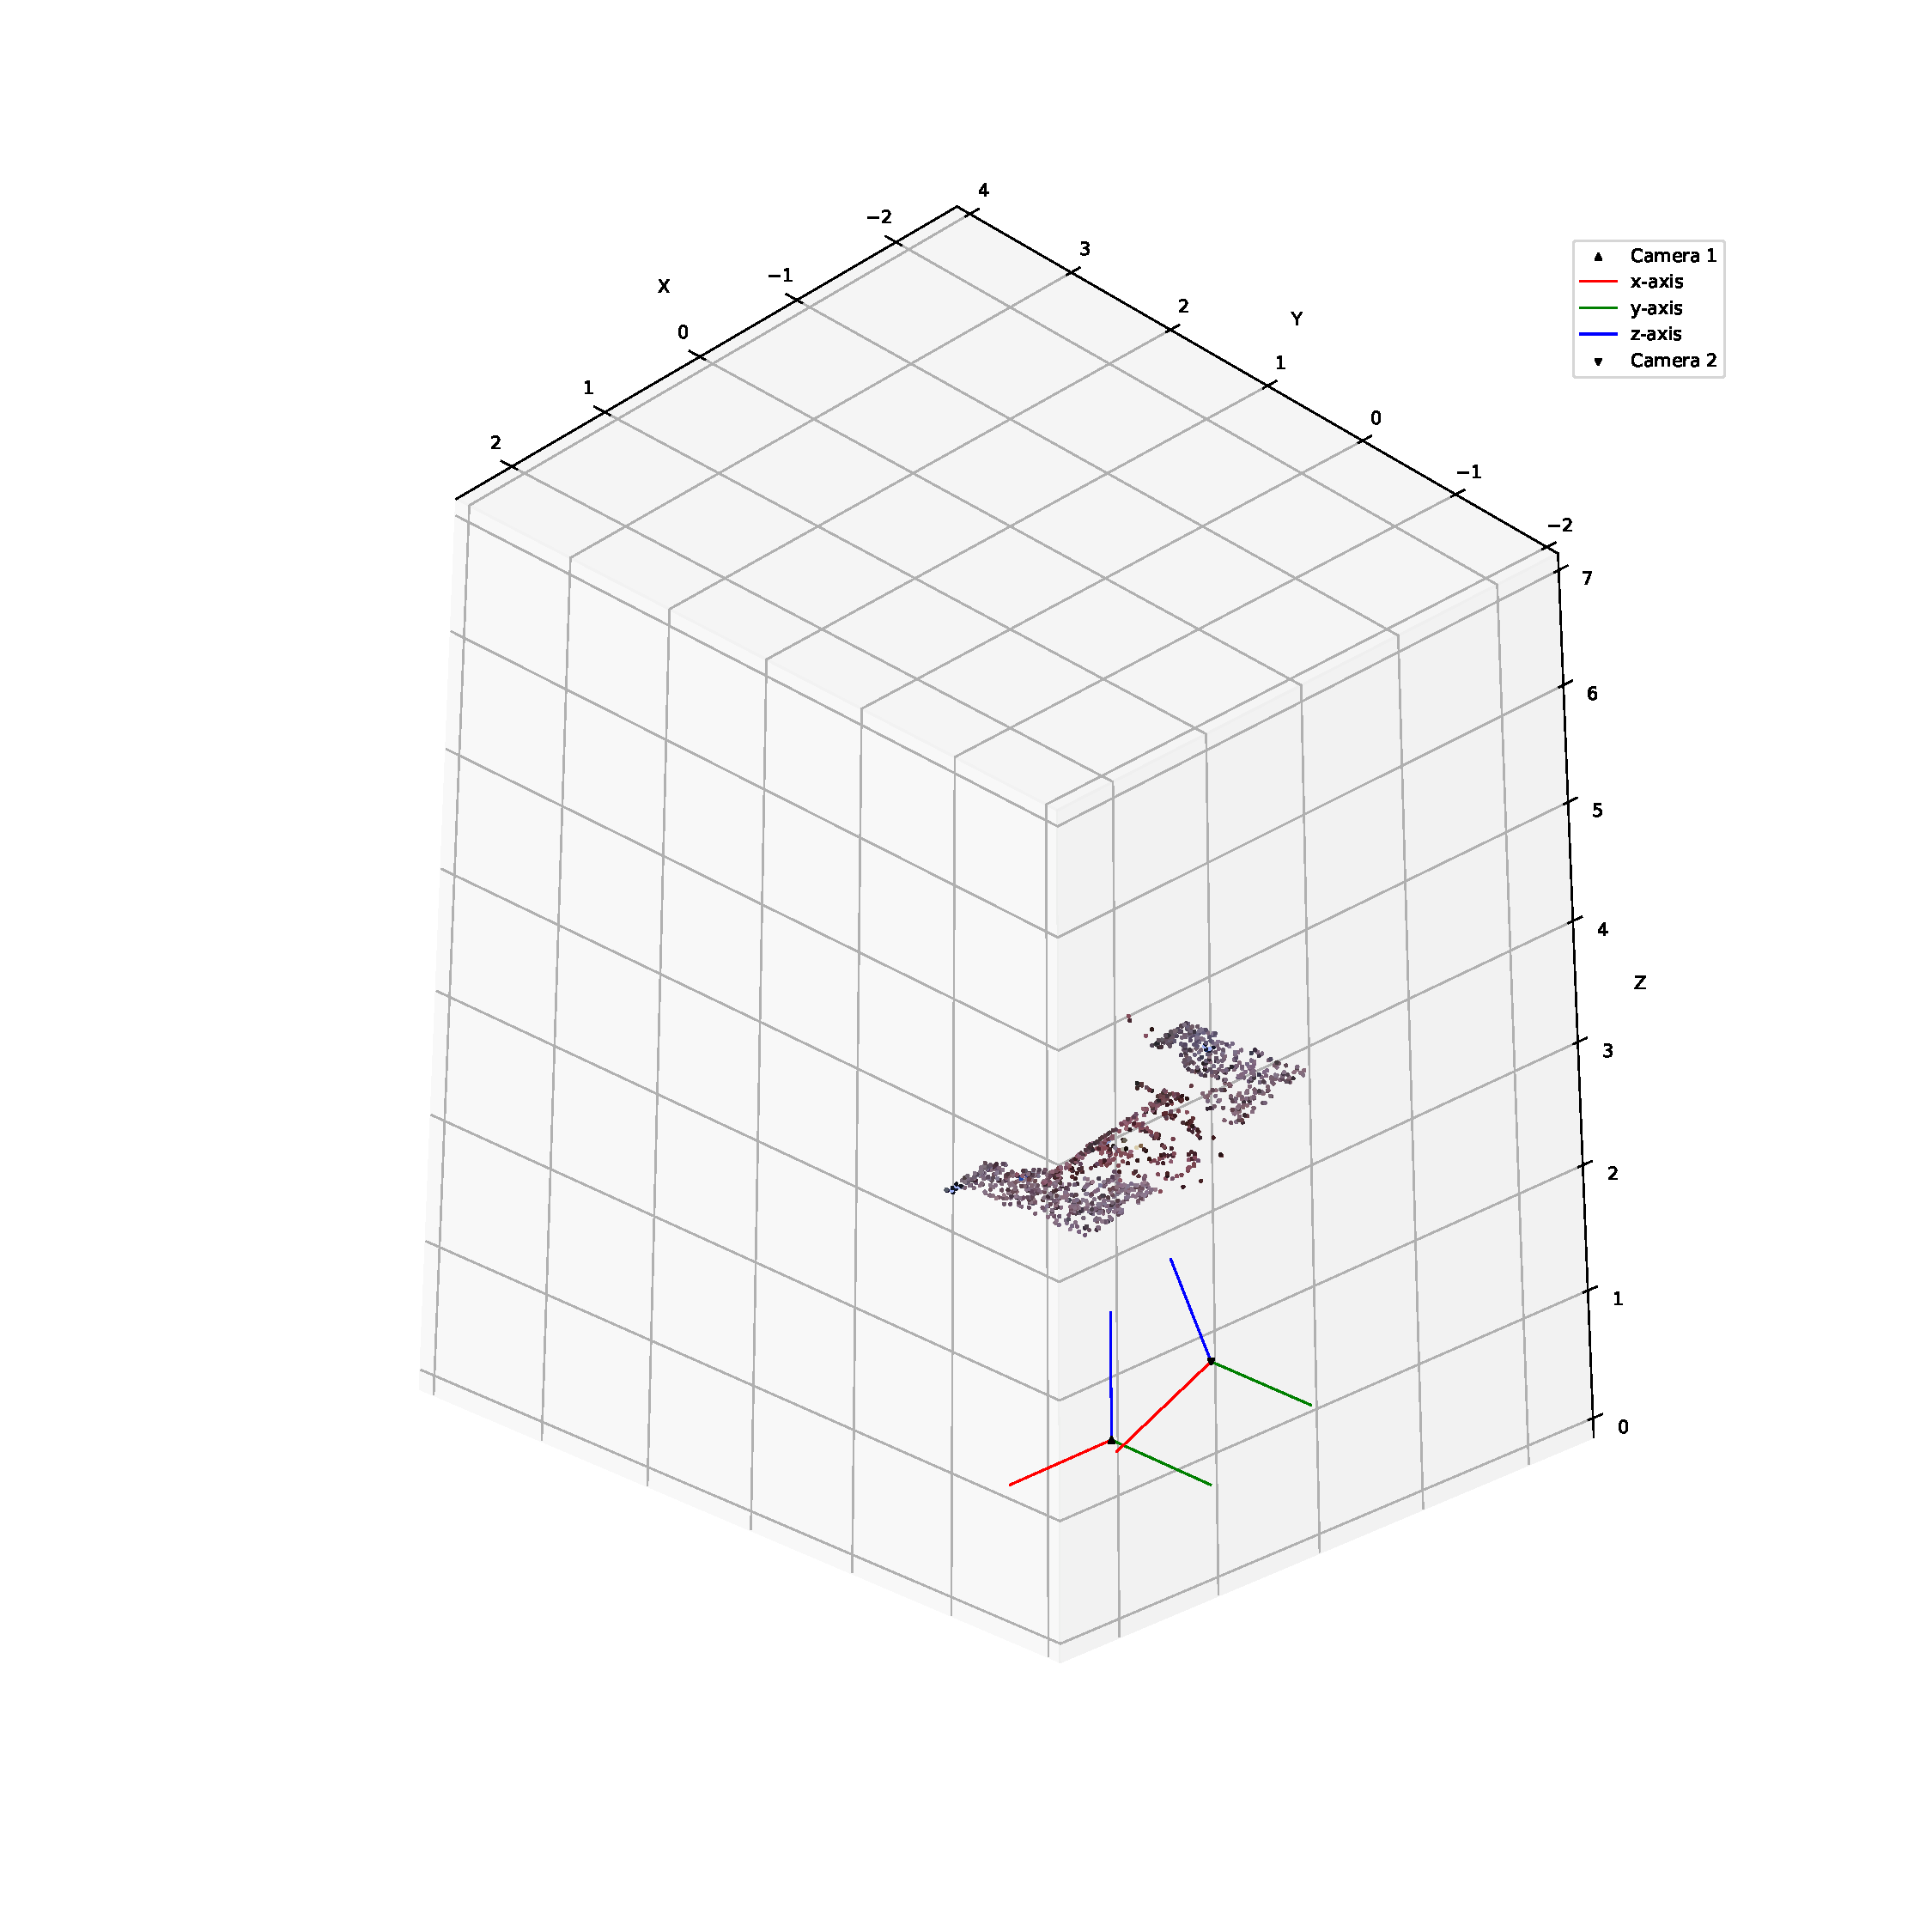
\includegraphics[width=\linewidth]{/home/madhia/computer_vision/assignment4/implementation/q3/output/fountain_3d_-30-135.pdf}
        \caption{Figure 2}
    \end{minipage}%
\end{figure}

\begin{figure}[h!]
    \centering
    \begin{minipage}{0.4\textwidth}
        \centering
        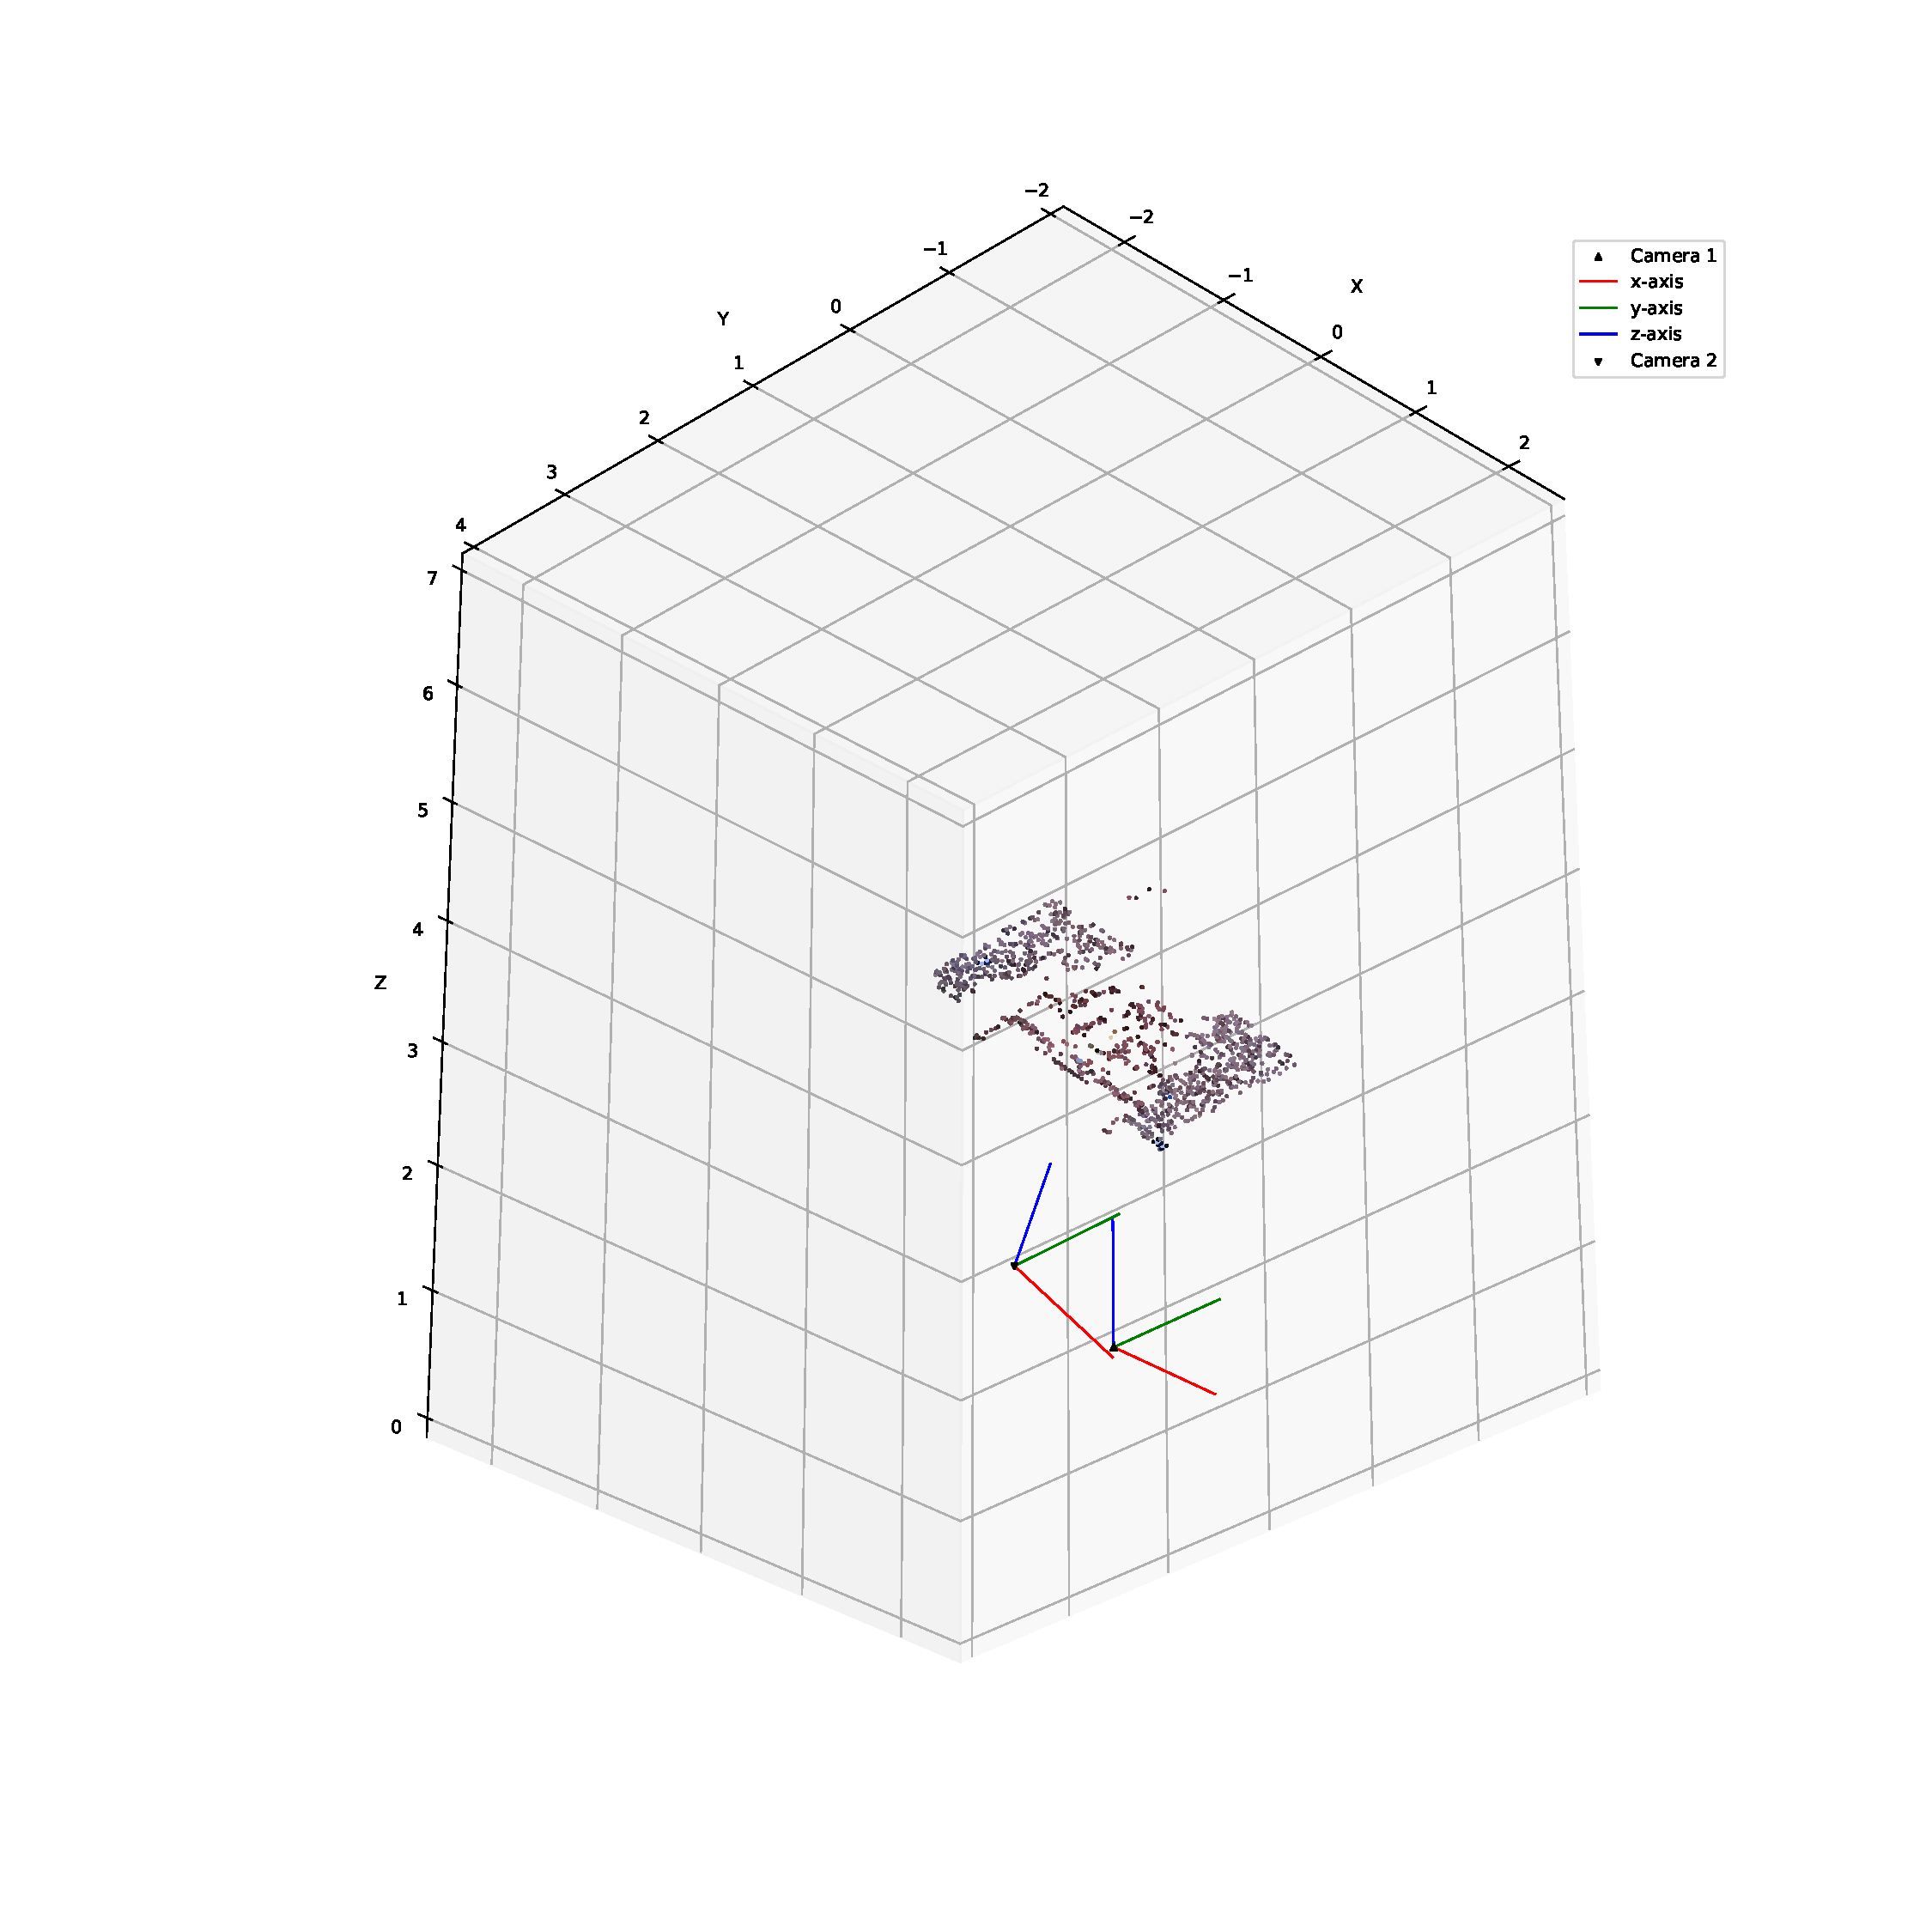
\includegraphics[width=\linewidth]{/home/madhia/computer_vision/assignment4/implementation/q3/output/fountain_3d_-30-225.pdf}
        \caption{Figure 3}
    \end{minipage}%
    \begin{minipage}{0.4\textwidth}
        \centering
        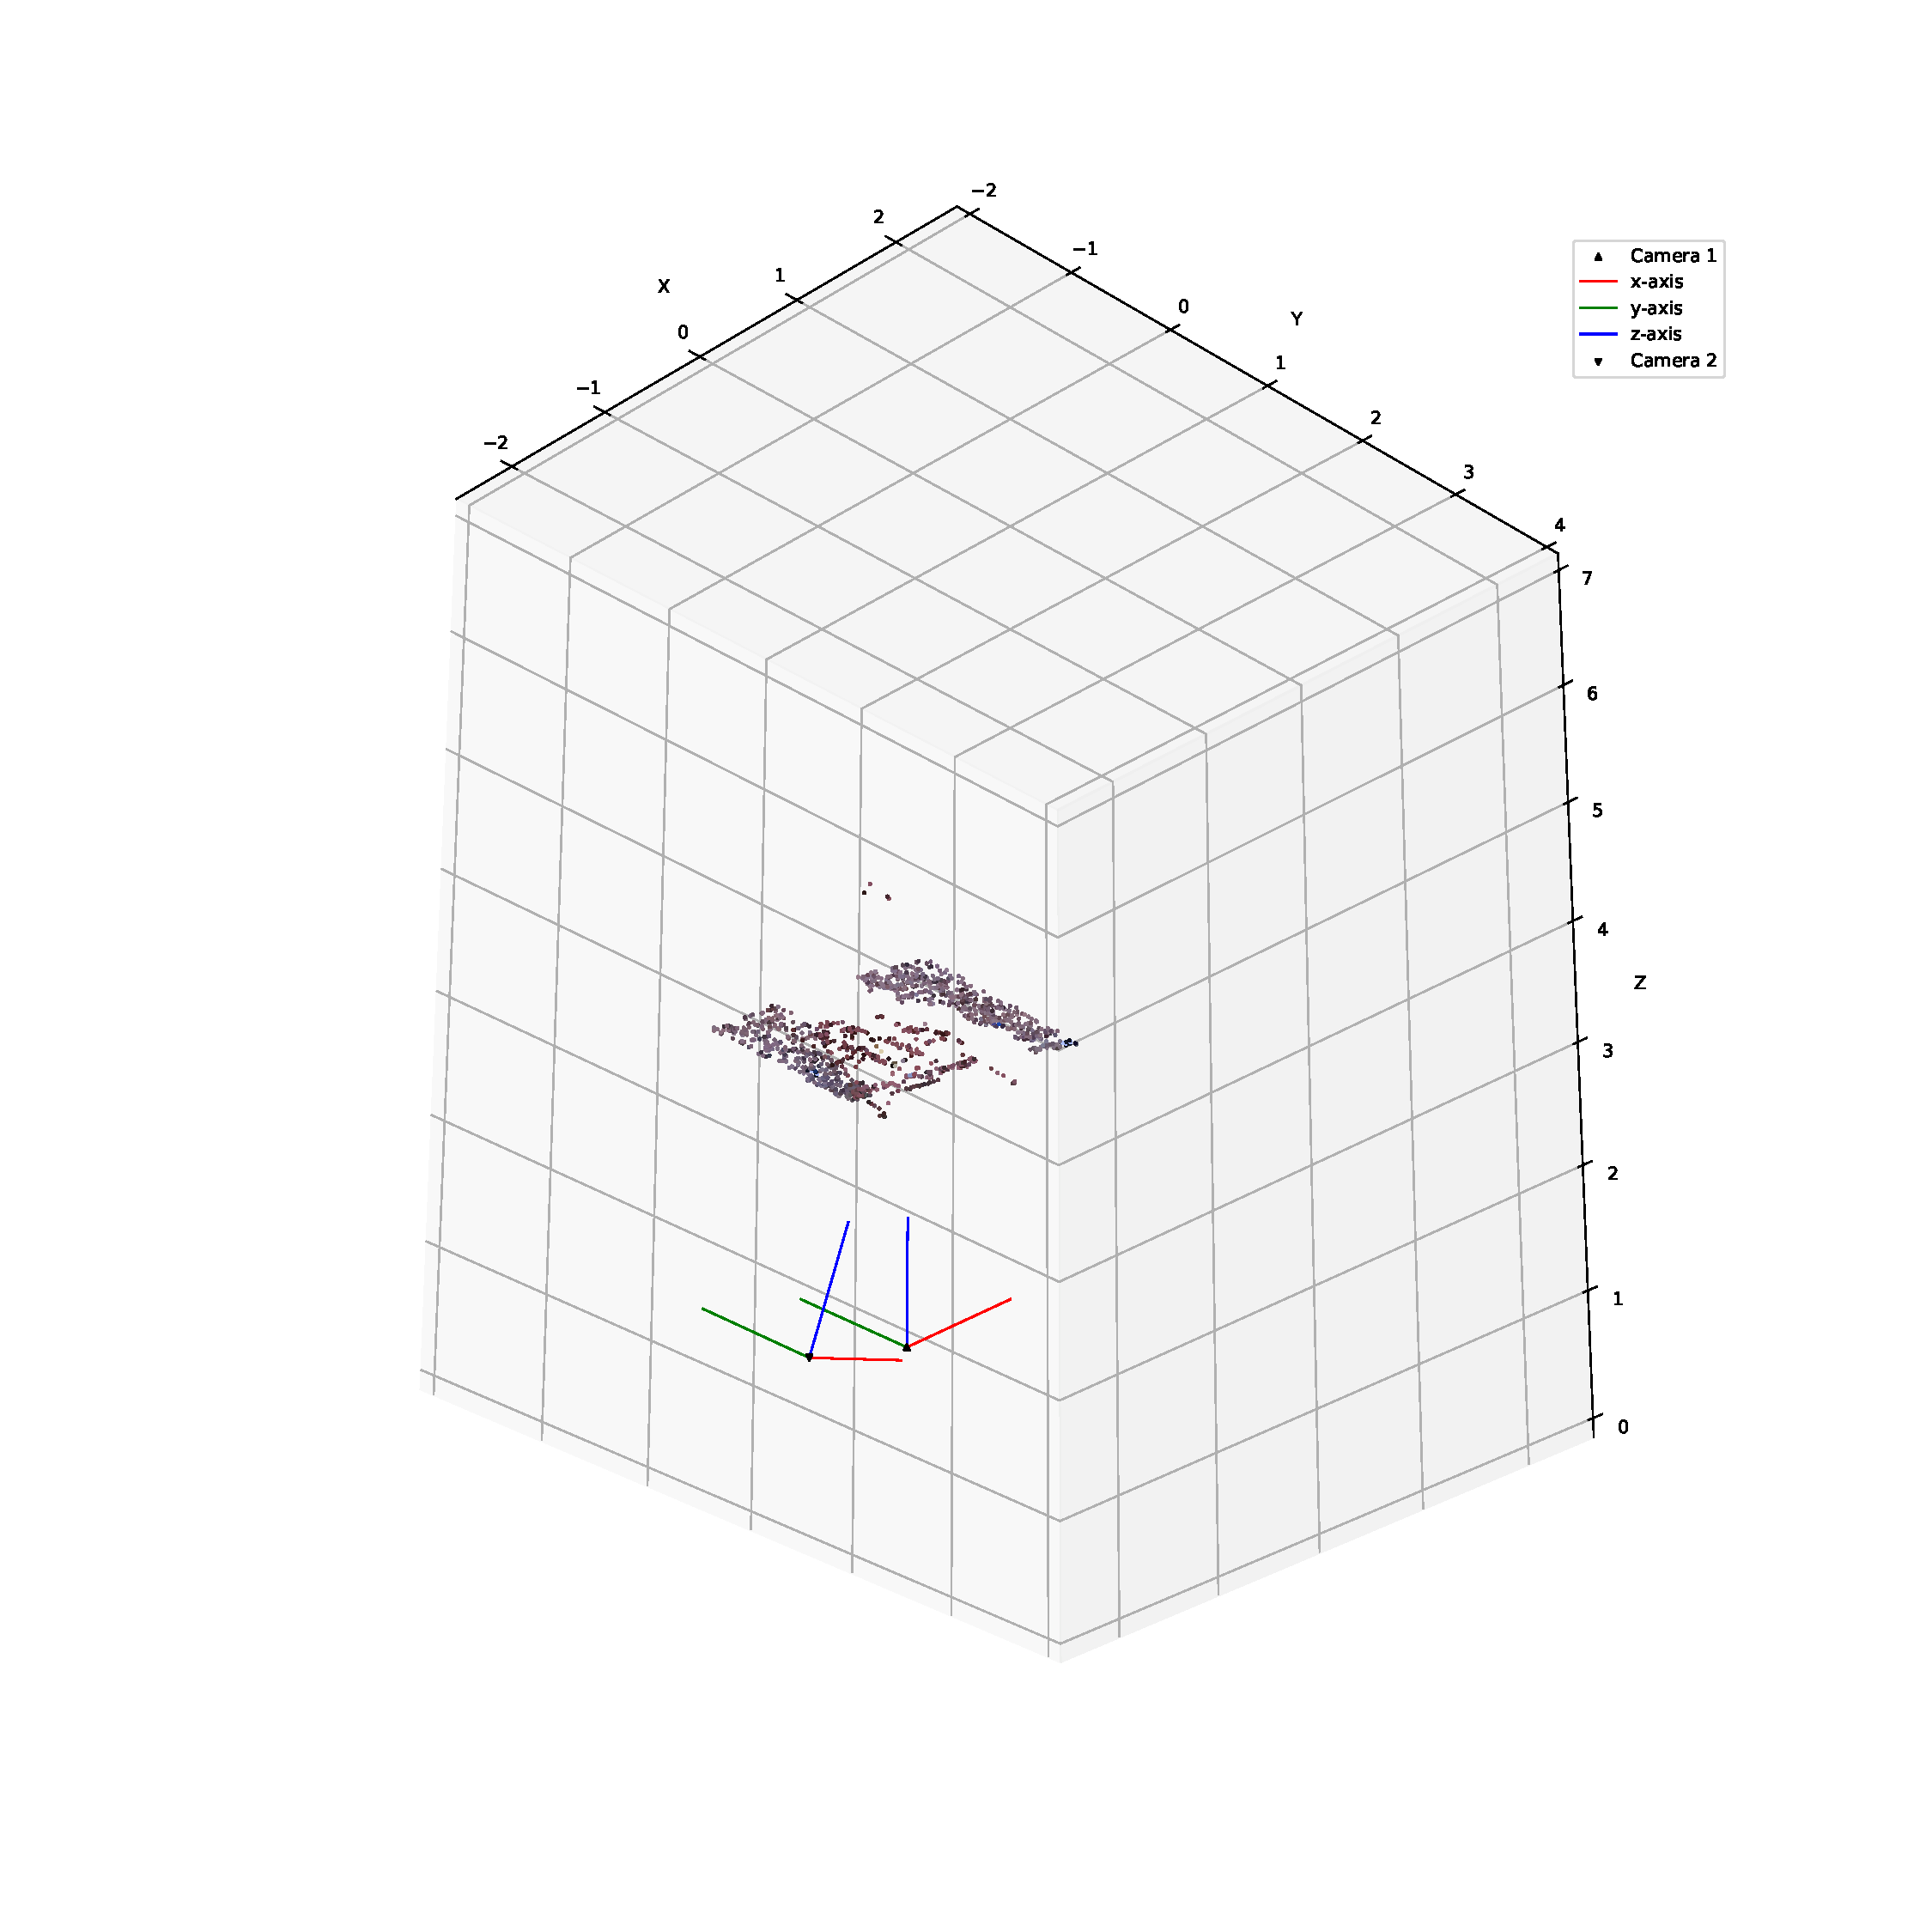
\includegraphics[width=\linewidth]{/home/madhia/computer_vision/assignment4/implementation/q3/output/fountain_3d_-30-315.pdf}
        \caption{Figure 4}
    \end{minipage}%
\end{figure}
    
\begin{figure}[h!]
    \centering    
    \begin{minipage}{0.4\textwidth}
        \centering
        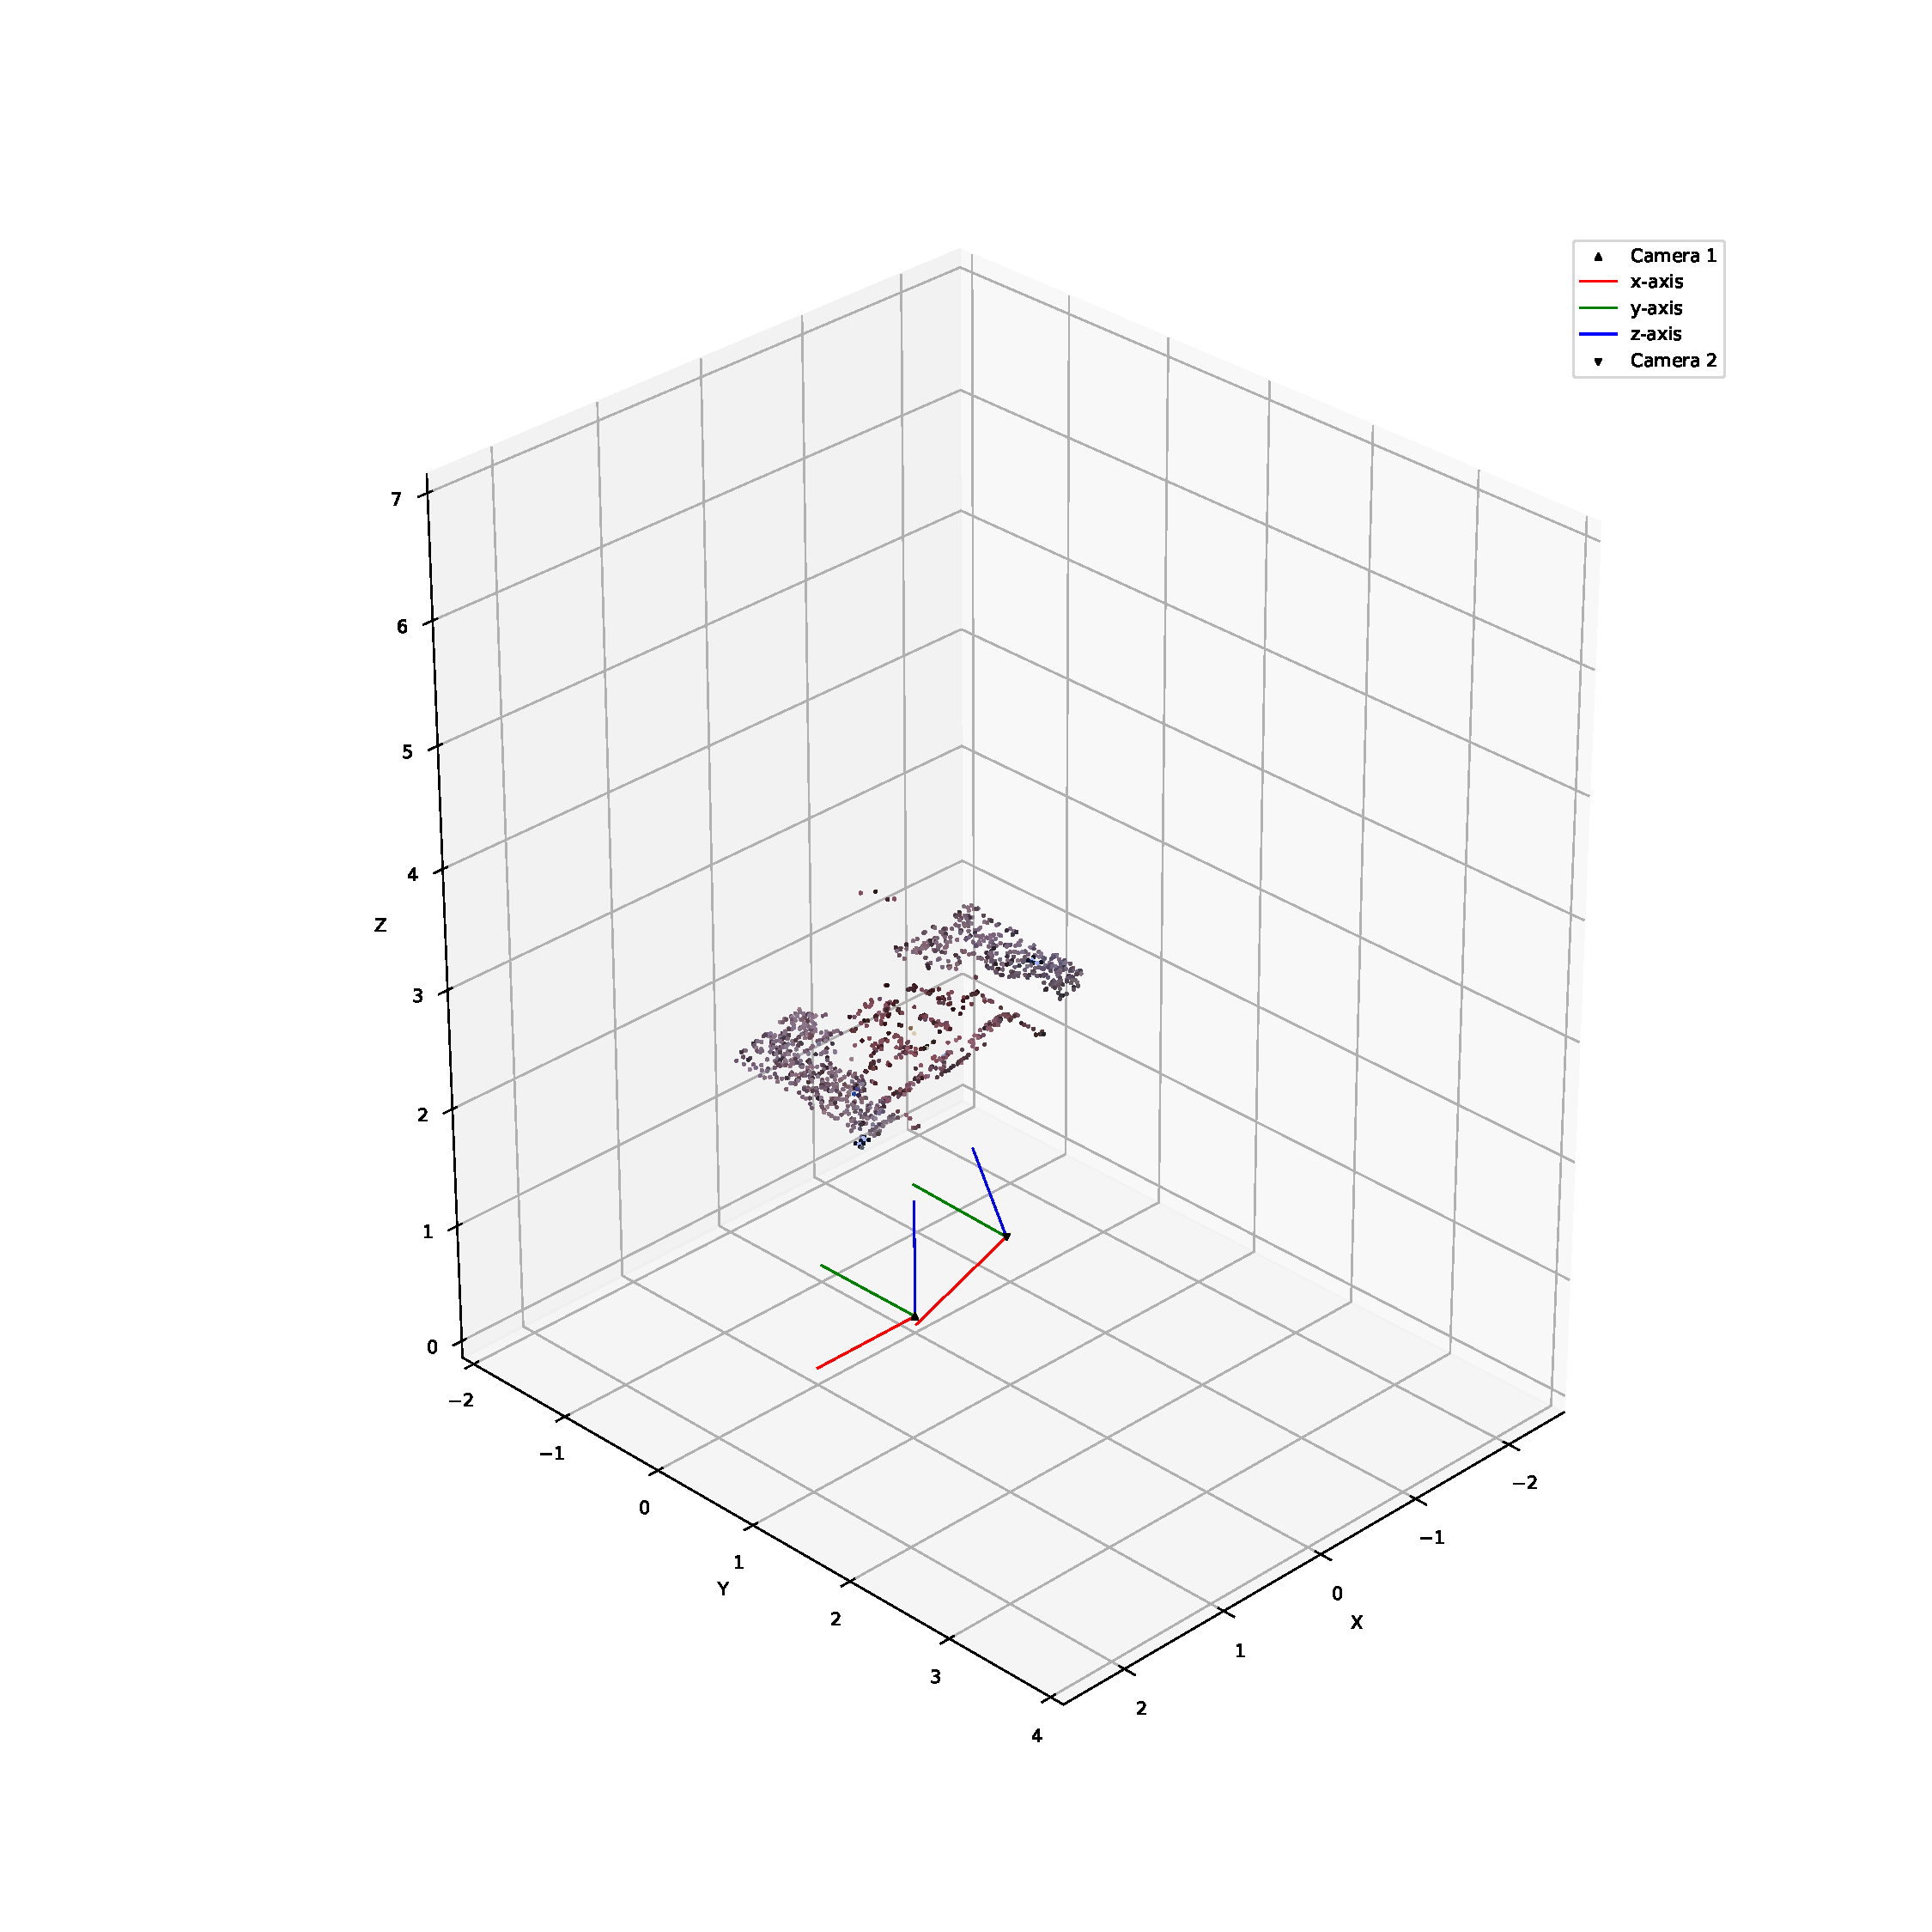
\includegraphics[width=\linewidth]{/home/madhia/computer_vision/assignment4/implementation/q3/output/fountain_3d_30-45.pdf}
        \caption{Figure 5}
    \end{minipage}%
    \begin{minipage}{0.4\textwidth}
        \centering
        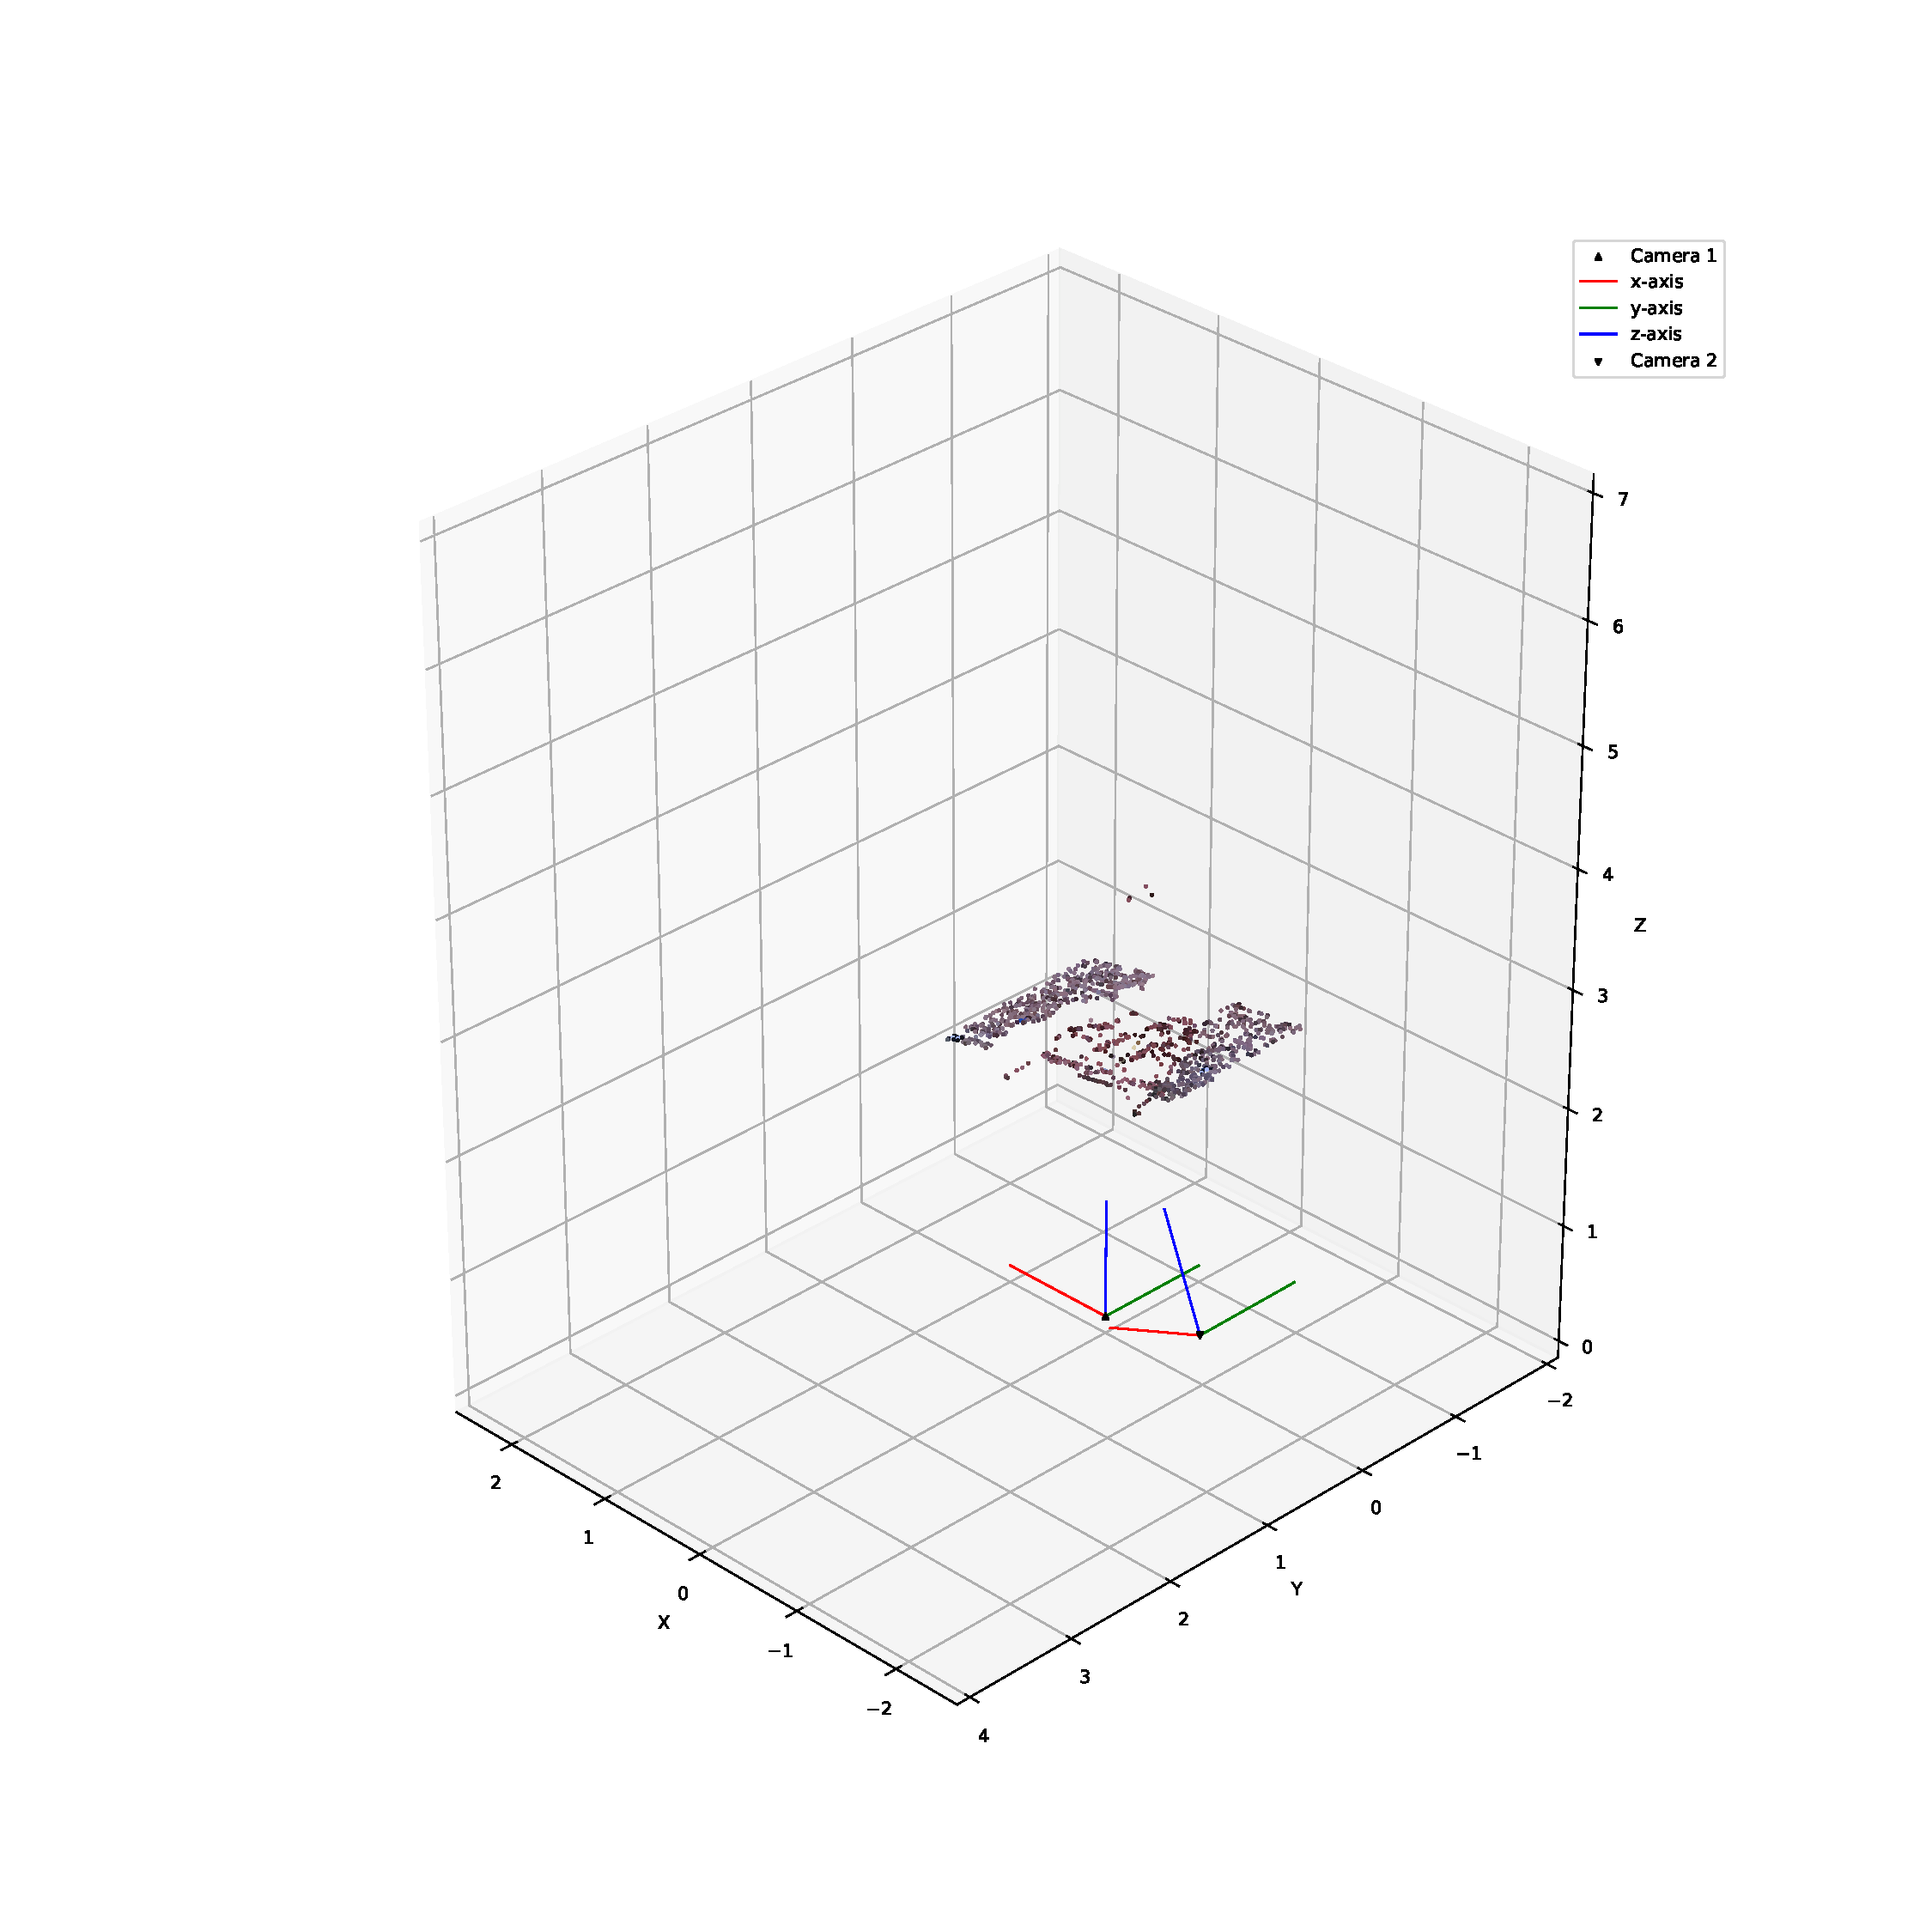
\includegraphics[width=\linewidth]{/home/madhia/computer_vision/assignment4/implementation/q3/output/fountain_3d_30-135.pdf}
        \caption{Figure 6}
    \end{minipage}%
\end{figure}
    
\begin{figure}[h!]
    \centering    
    \begin{minipage}{0.4\textwidth}
        \centering
        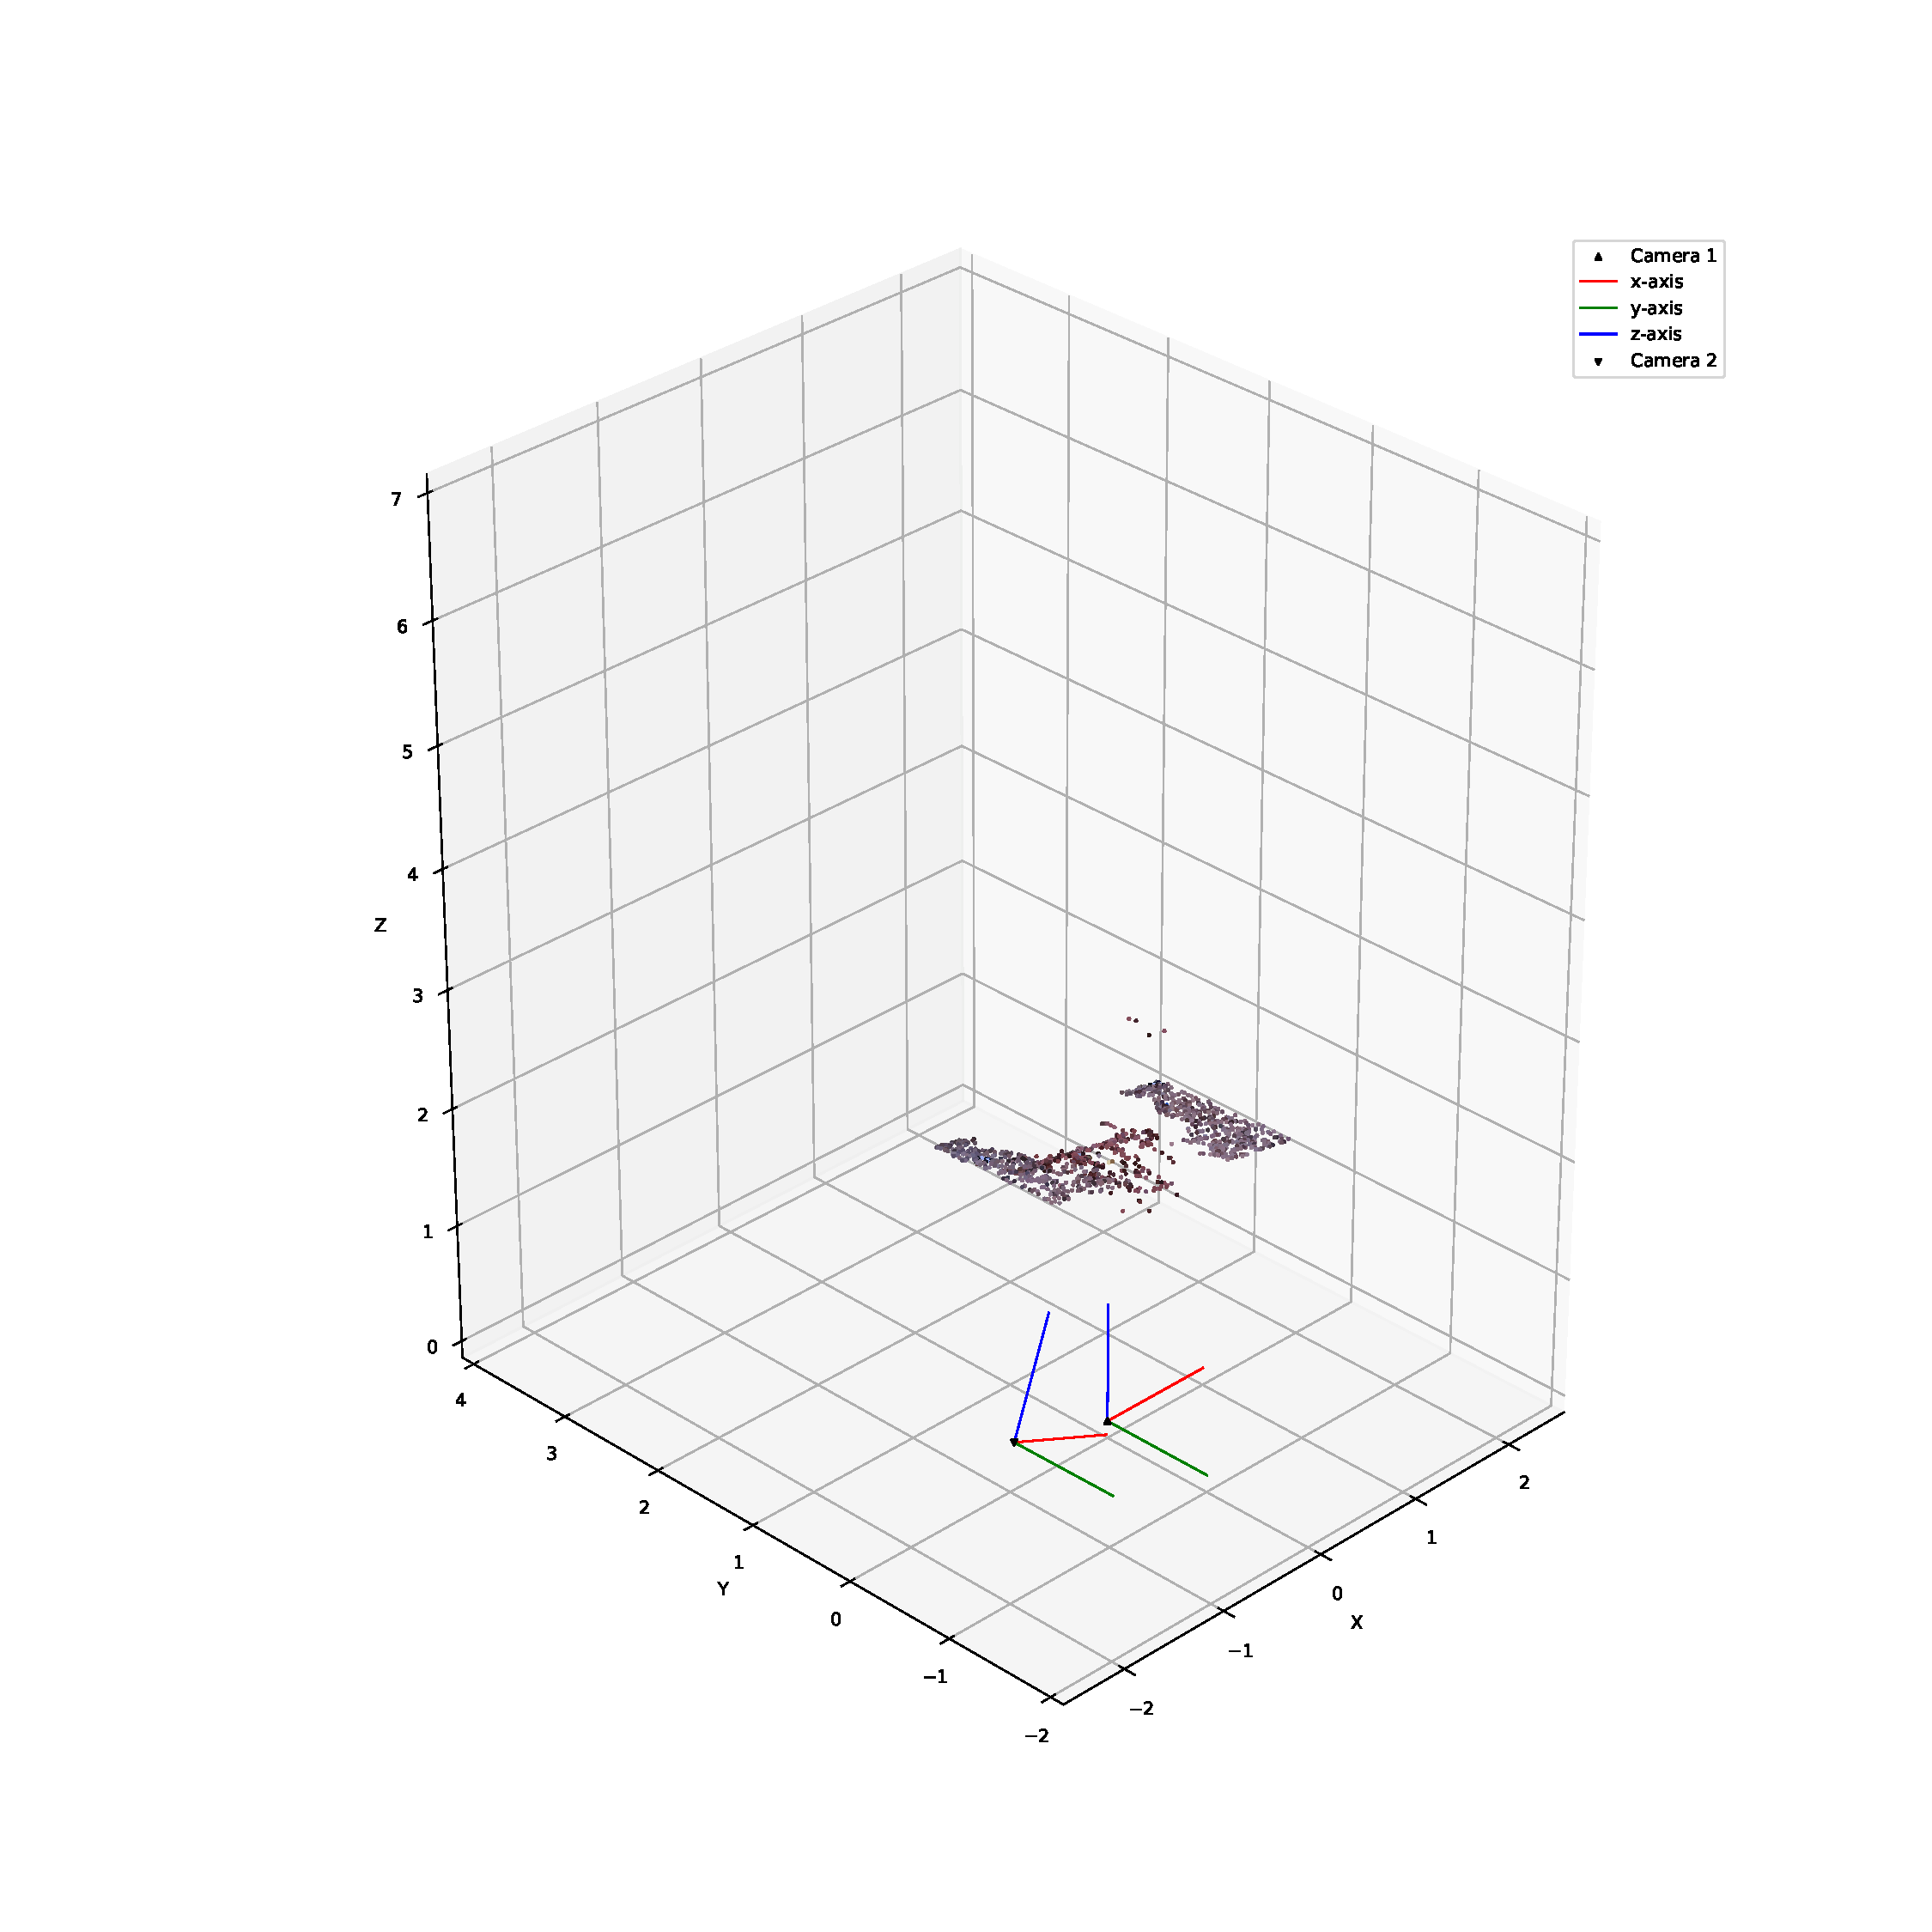
\includegraphics[width=\linewidth]{/home/madhia/computer_vision/assignment4/implementation/q3/output/fountain_3d_30-225.pdf}
        \caption{Figure 7}
    \end{minipage}%
    \begin{minipage}{0.4\textwidth}
        \centering
        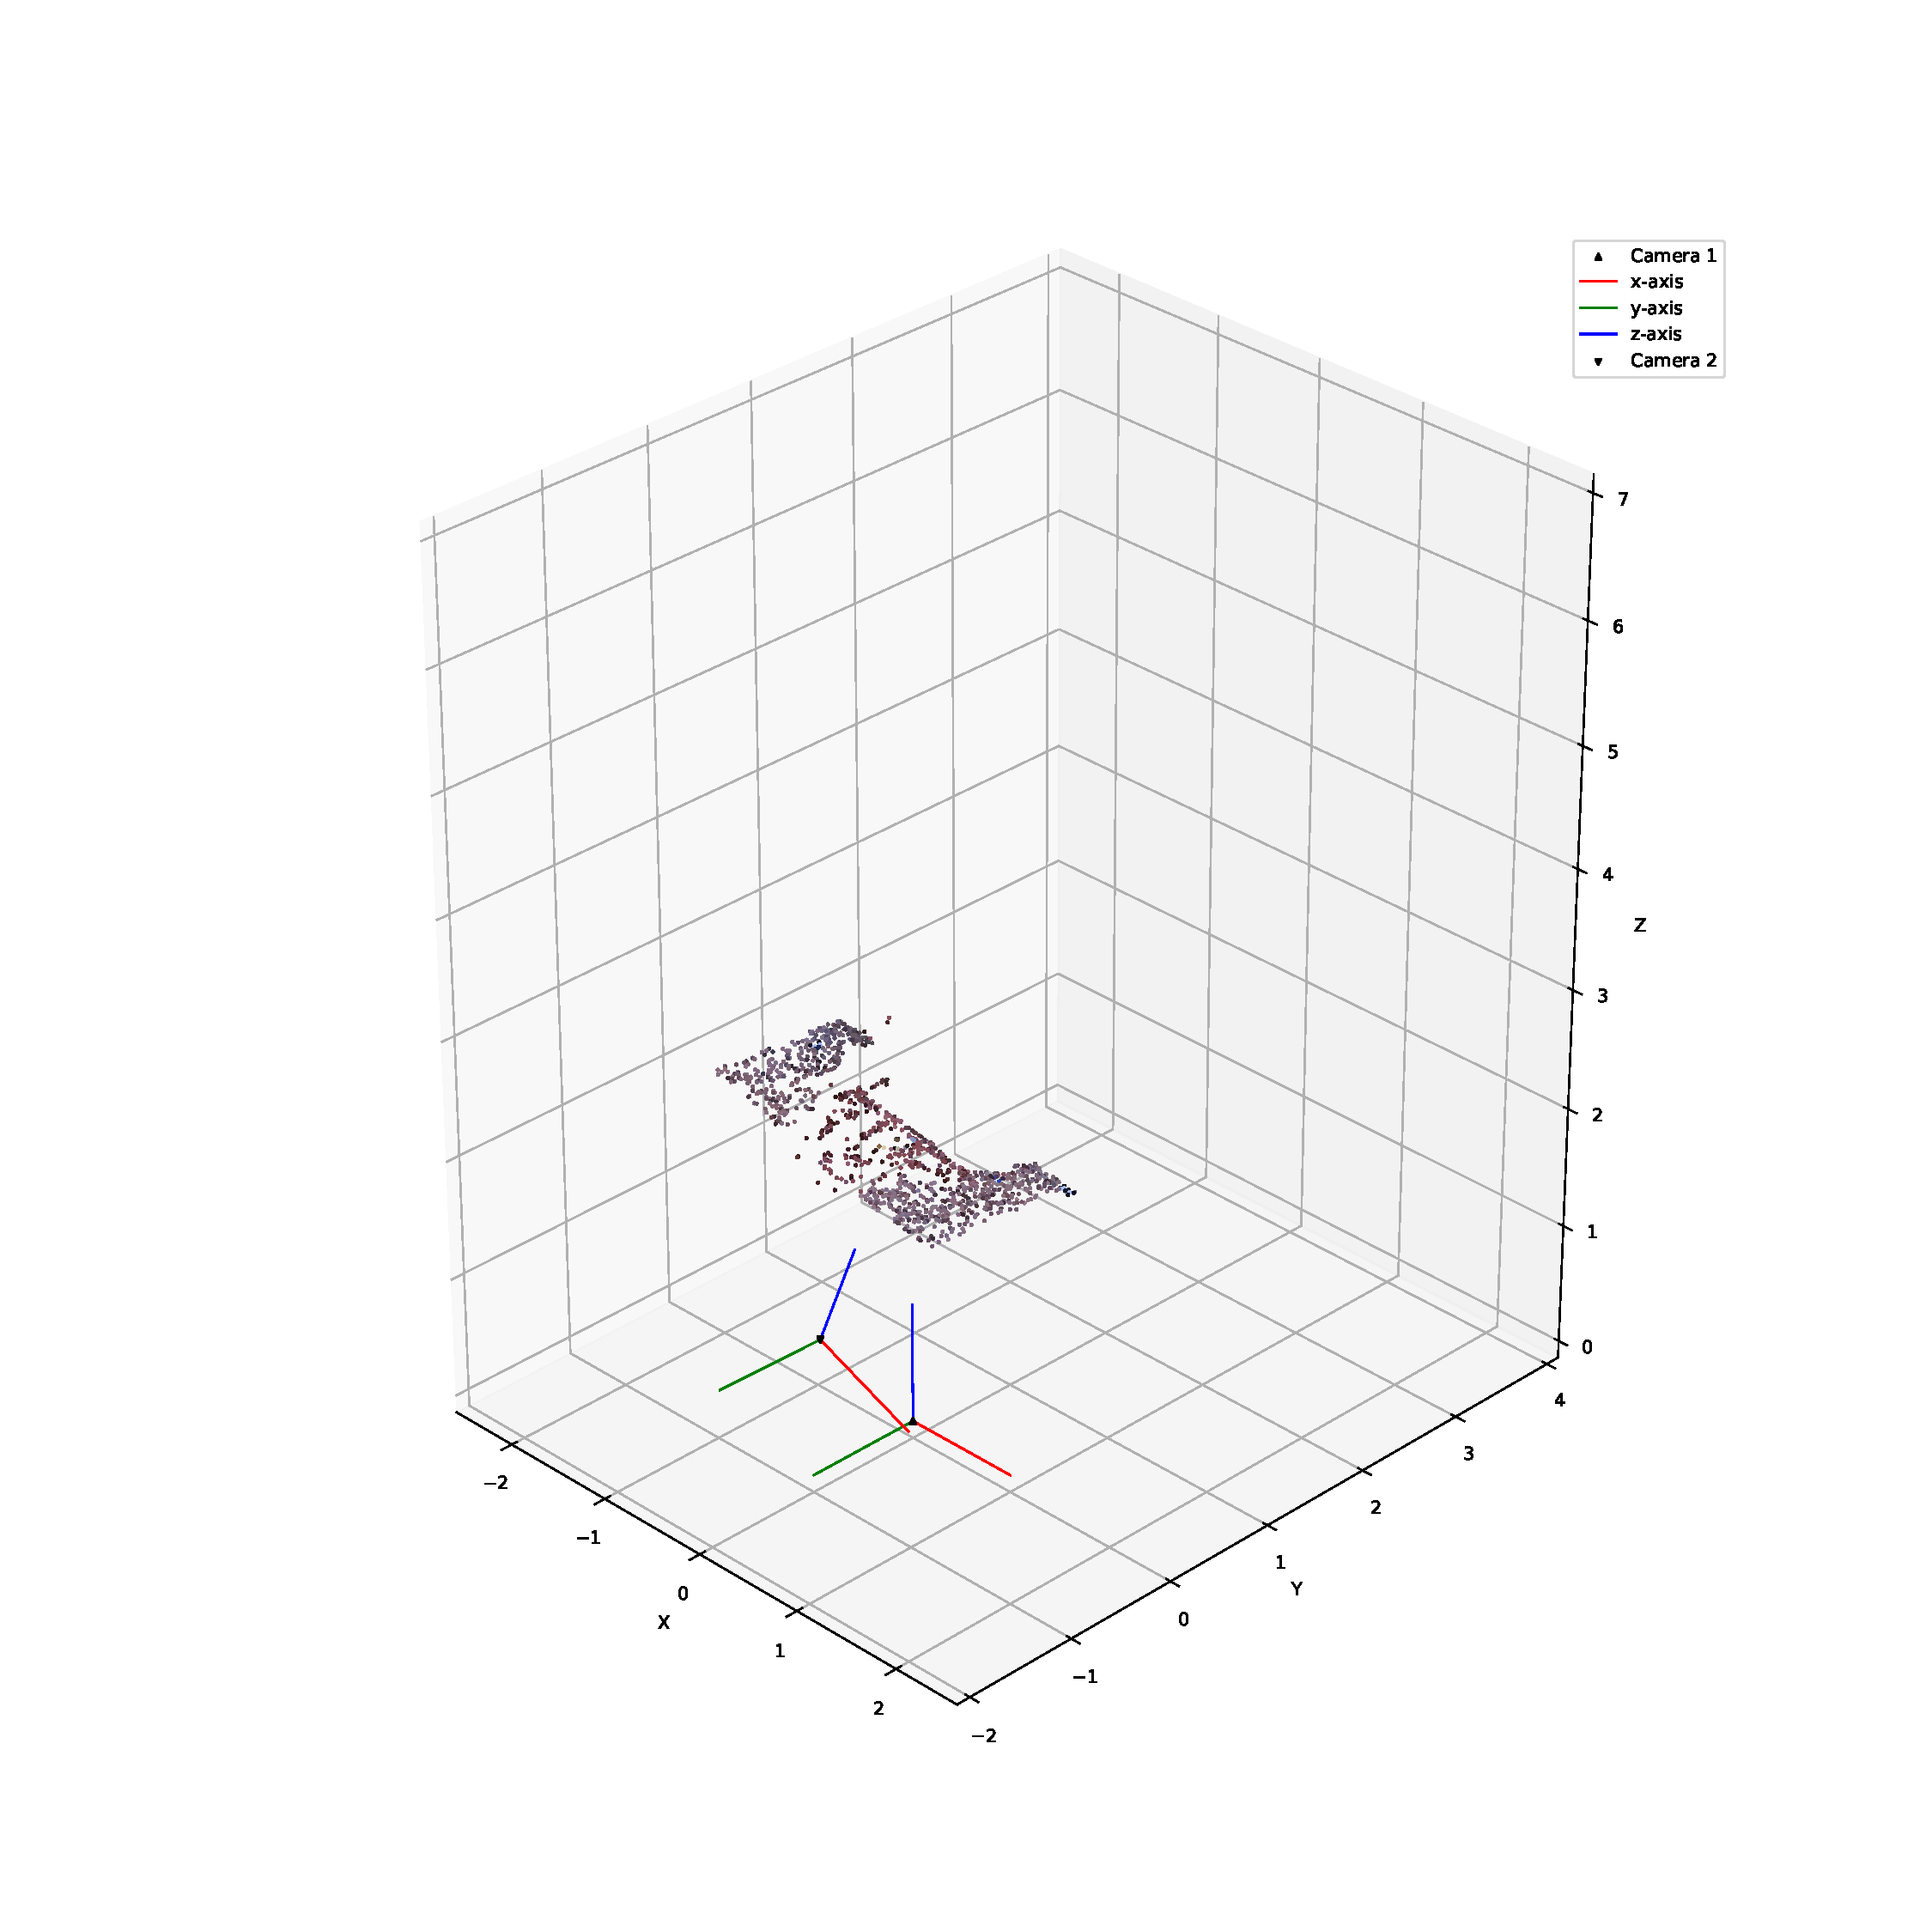
\includegraphics[width=\linewidth]{/home/madhia/computer_vision/assignment4/implementation/q3/output/fountain_3d_30-315.pdf}
        \caption{Figure 8}
    \end{minipage}
    \caption{Eight Figures Side by Side}
\end{figure}

\begin{figure}[h!]
    \centering    
    \begin{minipage}{0.4\textwidth}
        \centering
        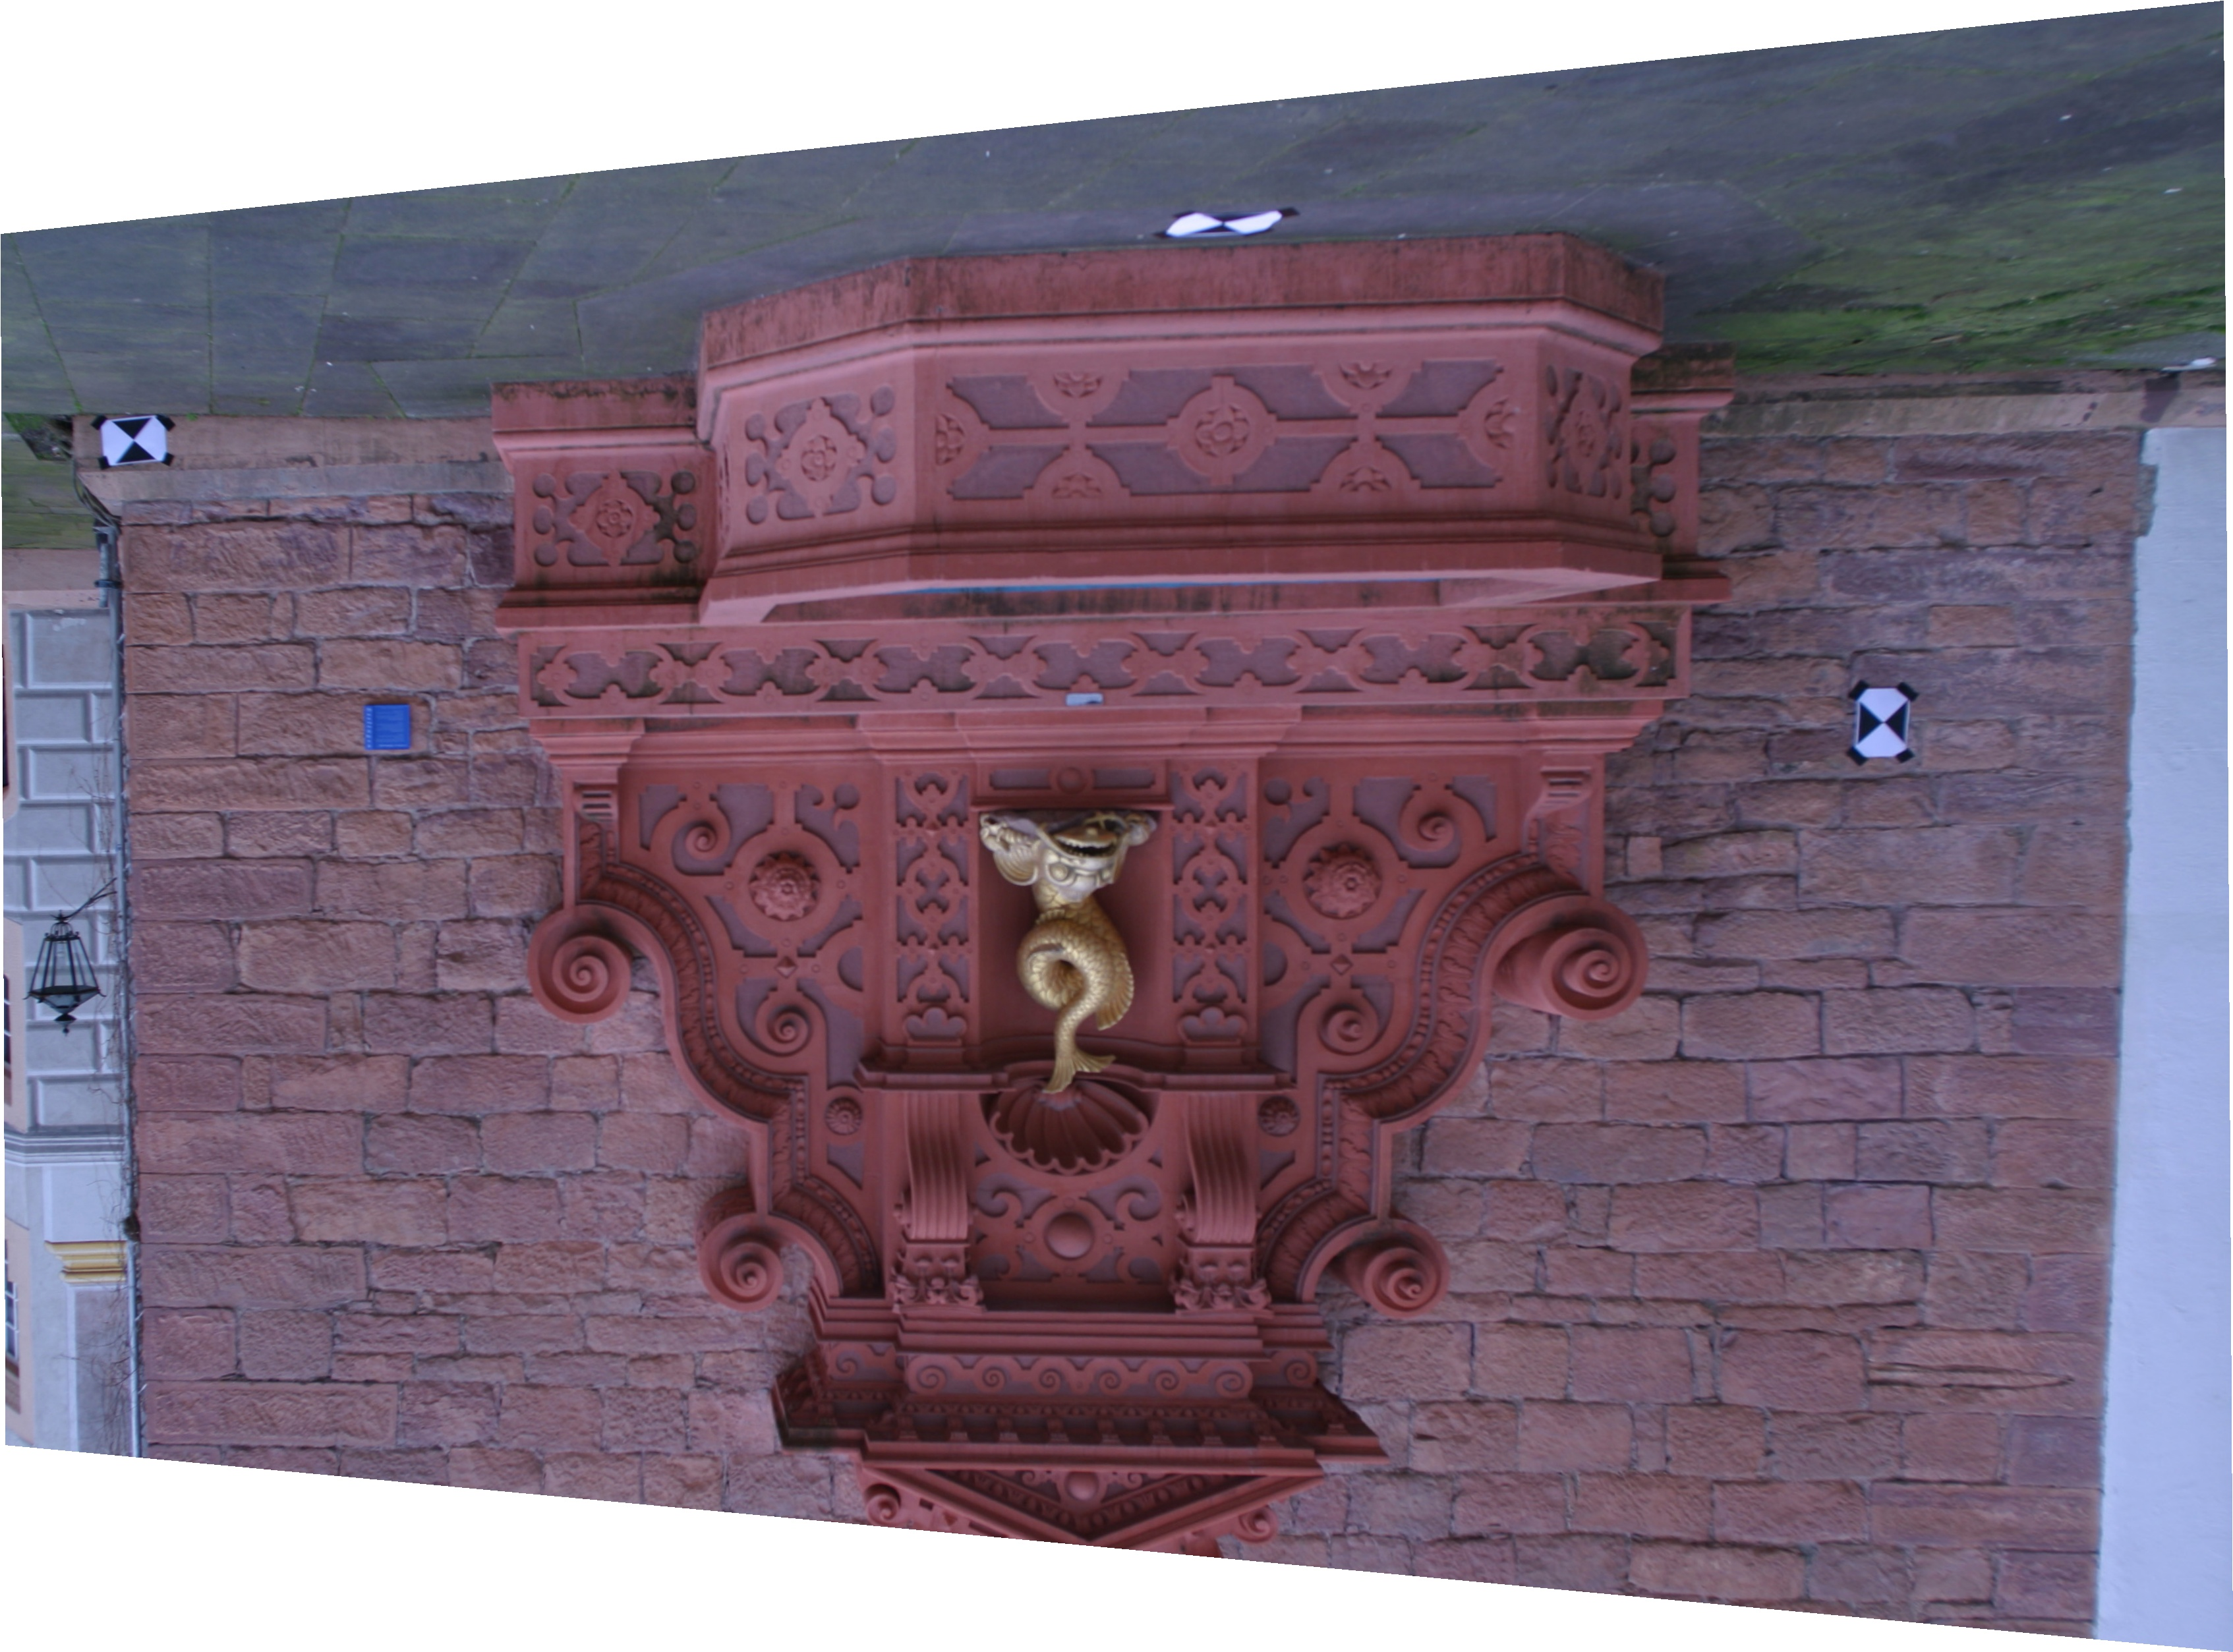
\includegraphics[width=\linewidth]{/home/madhia/computer_vision/assignment4/implementation/q3/output/fountain1_t.jpg}
        \caption{Figure 7}
    \end{minipage}%
    \begin{minipage}{0.4\textwidth}
        \centering
        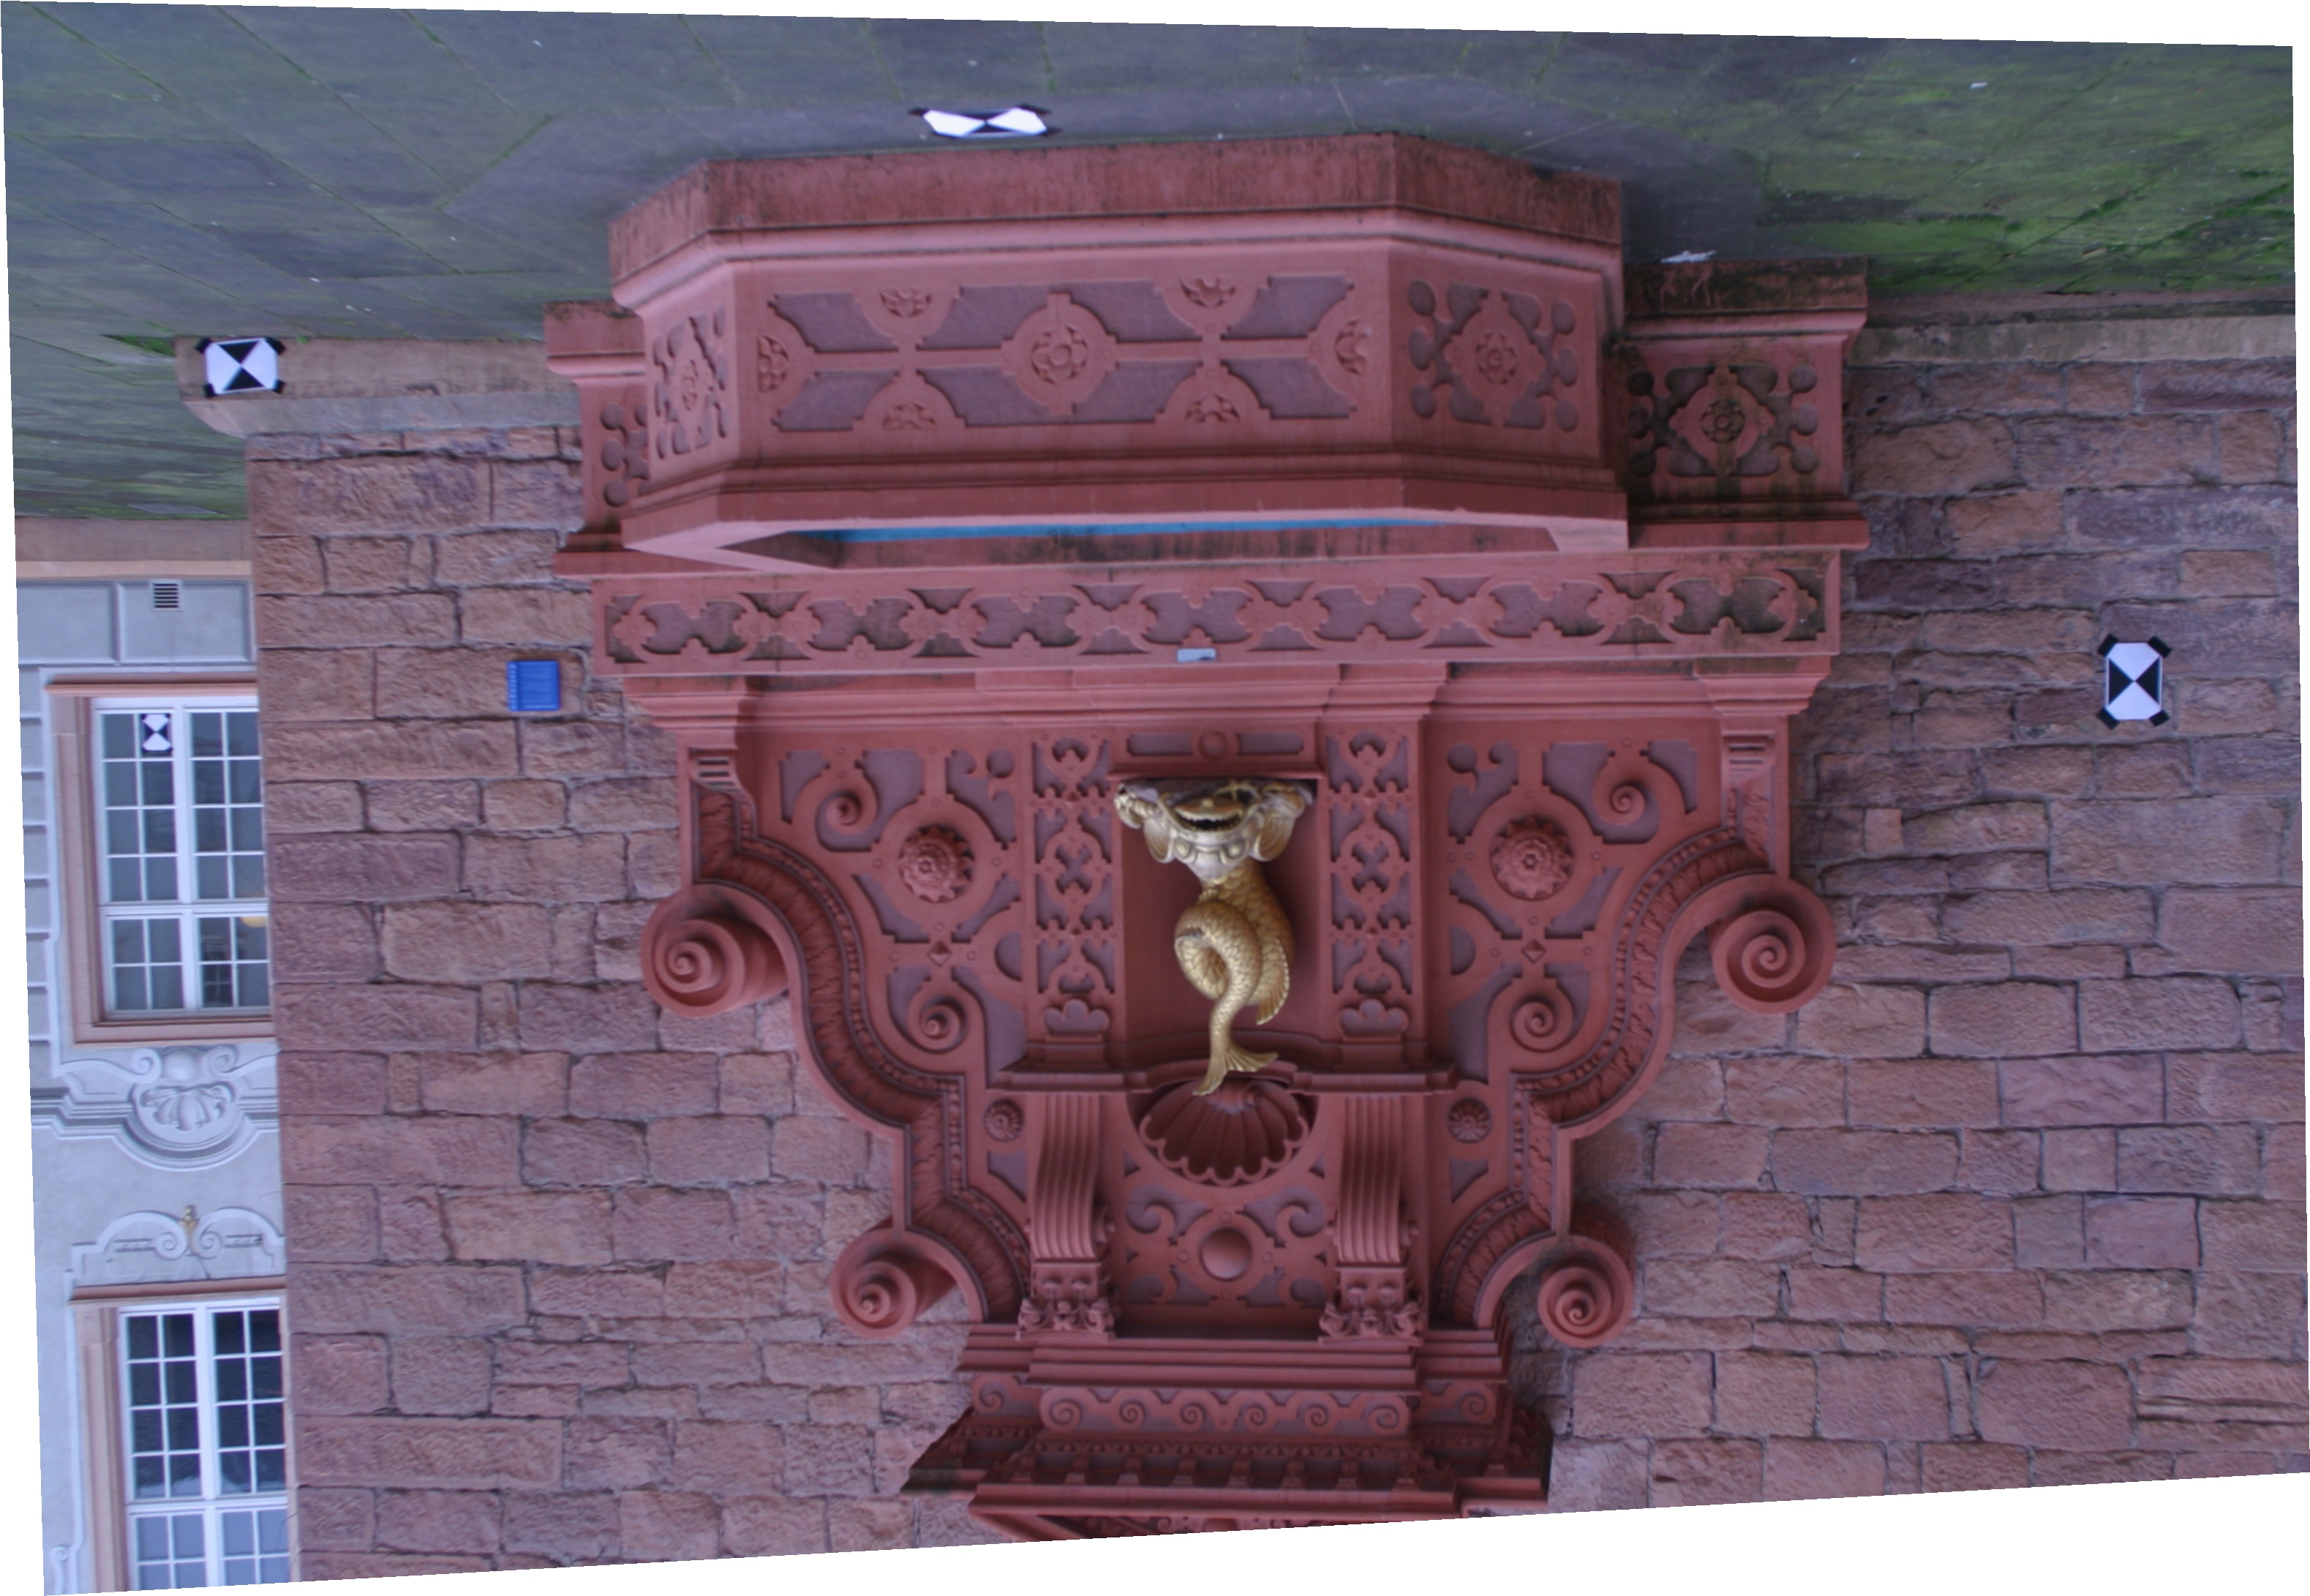
\includegraphics[width=\linewidth]{/home/madhia/computer_vision/assignment4/implementation/q3/output/fountain2_t.jpg}
        \caption{Figure 8}
    \end{minipage}
    \caption{Eight Figures Side by Side}
\end{figure}

\subsection{Discussion}
Briefly discuss how the results differ from the initial dataset and any challenges encountered.

\end{document}